\clearpage
\newpage
\chapter{Systematic Uncertainties}
\label{sec:systematics}
Various systematics are taken into account, both 
on our expected signal and background estimate. Some systematic uncertainties will affect only the normalization of certain event rates, 
and are reported as overall normalization uncertainties. Other systematics affect the shapes of the reconstructed signal or backgrounds, as well as their normalization.  The
Systematic uncertainties that are used in the analysis are summarized in table \ref{table:nuisance}.% All systematic effects are listed in Table \ref{table:systeffects}.

%\begin{sidewaystable}
%\begin{center}
%\begin{small}
%\begin{tabular}{| c || c || c | c | c  c  c  c  c  c  c  c |}
%\hline
%& \textbf{Process:} & $t\overline{t}$ & QCD & & & & & & & &\\
%& \textbf{$W^\prime$ Mass Point:} & & & 1300 & 1500 & 1700 & 1900 & 2100 & 2300 & 2700 & 3100  \\
%\hline
%\textbf{Systematic} & \textbf{Variation ($\%$)} & \multicolumn{9}{c}{\textbf{Effect of Systematic} (\%)} \\ 
%\hline
%Luminosity & $\pm 4.4$ & 4.4 &  & 4.4 & 4.4 & 4.4 & 4.4 & 4.4 & 4.4 & 4.4 & 4.4 \\
%Subjet Scale Factor & $\pm 5$ & 5 &  & 5 & 5 & 5 & 5 & 5 & 5 & 5 & 5 \\
%$t\overline{t}$ cross-section & $\pm 50$ & 50 & & & & & & & & & \\
%b-tagging & see text & 7 & & 8 & 8 & 9 & 9 & 11 & 11 & 12 & 10  \\
%Trigger Efficiency & see text & 7 & & 1 & $<1$ & $<1$ & $<1$ & $<$1 & $<1$ & $<1$ & $<1$  \\
%Jet Energy Scale$^{up}_{down}$ & $\pm 5$ & $^{22}_{20}$ & & $^{7}_{11}$ & $^{1}_{4}$ & $^{1}_{2}$ & $^{12}_{0.1}$ & $^{4}_{1}$ & $^{4}_{1}$ & $^{4}_{1}$ & $^{0.5}_{3}$  \\
%QCD Systematic & see text & & 4 & & & & & & & &  \\
%\hline
%Number of Events& & 1042 & 17901 & 579 & 274 & 118 & 51 & 22 & 10 & 2 & 1 \\
%\hline
%\end{tabular}
%\caption{Effect of systematics listed in Section \ref{sec:systematics}, computed over the entire mass-range.  The b-tagging, Jet Energy Scale, and Trigger uncertainties have non negligible 
%shape based effects that must be taken into account. Note: the $2\%$ b-tagging systematic derived in Section \ref{sec:btagging} is included in the b-tagging line above.}
%\label{table:systeffects}
%\end{small}
%\end{center}
%\end{sidewaystable}

\section{Jet Energy Scale}
We evaluate the effect of uncertainty on the jet energy scale on samples derived from MC simulation.  
To do so, we vary the jet four-momentum up and down by the jet energy 
scale uncertainty, which we take to be $3\%$. We include $\pt$ and $\eta$ dependent corrections to the 
jet energies, as well as uncertainties from the difference in measured and simulated $W$ masses \cite{ZP8TeV}. 

Varying the jet momentum can cause a jet to fall below or rise above the $\pt$ cut in the analysis, thus shifting the invariant 
mass spectrum of the signal and reconstructed $\ttbar$ samples. Figure \ref{figs:ttbarJES} shows the systematic shapes from the 
jet energy scale on the $\ttbar$ distribution.  Jet Energy scale variation on signal MC is shown in Figure \ref{figs:signalJES} for 1300$~\GeV$,
 1900$~\GeV$, and 2300$~\GeV$ mass points.

\section{Trigger}
We include an uncertainty based on the measured trigger efficiency for all MC Samples. The trigger efficiency is discussed in Section \ref{sec:trigger}. 
To obtain shape systematics from this effect, we vary the trigger by half the trigger \textit{in}efficiency. The effects of this on the $t\overline{t}$ 
distribution is shown in Figure \ref{figs:ttbartrig}. Trigger weighting on signal MC is shown in Figure \ref{figs:signaltrig} for 1300$~\GeV$,
 1900$~\GeV$, and 2300$~\GeV$ mass points.  The uncertainty is low in the mass range of interest for limit setting.

\section{Jet Energy Resolution}
\label{sec:JER}
We apply a systematic due to the known differences in jet energy resolution in data and simulation.  We use $\eta$ dependent smearing (see \cite{ZP8TeV}) as recommended by the JER group.  
We apply this systematic uncertainty to the $t\overline{t}$ distribution 
(as seen in Figure \ref{figs:ttbarJER}).  Jet Energy Resolution variation on signal MC is shown in Figure \ref{figs:signalJER} for 1300$~\GeV$,
 1900$~\GeV$, and 2300$~\GeV$ mass points. 

\section{Jet Angular Resolution}
A smearing of $10\%$ is assumed on $\eta$ and $\phi$ and shape uncertainties are generated by considering smearing $10\%$ 
lower and higher. We apply this systematic uncertainty to the $\ttbar$ distribution (as seen in Figure \ref{figs:ttbarJAR} ). Jet Angular Resolution 
variation on signal MC is shown in Figure \ref{figs:signalJAR} for 1300$~\GeV$,
 1900$~\GeV$, and 2300$~\GeV$ mass points.  The effect is very small and thus not considered in setting limits.

\section{PDF Uncertainty}
The uncertainty in the parton distribution function used for MC sample generation is investigated.  We take the average of the $\pm$1$\sigma$ eigenvalue 
variation of the pdf master equations \cite{Bourilkov:2006cj} 
for the NNPDF, MSTW2008nnlo, and CT10 pdf sets to weight the signal and $\ttbar$ MC samples and investigate the impact on the full selection.  The PDF set 
that provides the maximum uncertainty is then used for the $\pm$1$\sigma$ PDF uncertainty.  For $\ttbar$ and signal this set is NNPDF. PDF 
variation on signal MC is shown in Figure \ref{figs:signalPDF} for 1300$~\GeV$,
 1900$~\GeV$, and 2300$~\GeV$ mass points.  PDF variation on $\ttbar$ MC is shown in Figure \ref{figs:ttbarPDF}.  The effect is very small and thus not considered in setting limits.

\section{Pileup}
A study of pileup uncertainty is conducted by varying the minimum bias cross-section by 5\% as a measure of systematic uncertainty.  The results 
can be seen in figure \ref{figs:signalPU}.  The effect is very small and thus not considered in setting limits.

\section{b-Tagging Scale Factor Uncertainty}
\label{sec:btagunc}
The uncertainty in the b-tagging scale factor described in Section \ref{sec:btagging} is applied based on the b candidate pt.  The binning and associated errors 
listed below are the suggested EPS13 prescription generated from measurements in both muon-jet and ttbar data representing 20$~\fbinv$ of integrated 
luminosity.  The absolute uncertainty on $SF_b$ for a b candidate jet within the listed $\pt$ range is applied as shown in table \ref{table:btaggingerrors} 
for $\pt < 800~\GeV$.  B candidate jets with $\pt > 800~\GeV$ are assigned an uncertainty equal to twice the listed value for $600~\GeV < \pt < 800~\GeV$

\begin{table}
\begin{center}
\begin{tabular}{|l|r|} 
\hline
\bf{$\pt$ range } & \bf{Absolute Error on $SF_b$} \\
\hline
$320~\GeV < \pt < 400~\GeV$ & 0.0313175 \\
$400~\GeV < \pt < 500~\GeV$ & 0.0415417 \\
$500~\GeV < \pt < 600~\GeV$ & 0.0740446 \\
$600~\GeV < \pt < 800~\GeV$ & 0.0596716 \\
\hline
\end{tabular}
\end{center}
\caption{Absolute Error applied to the b-tagging Scale Factor}
\label{table:btaggingerrors}
\end{table}


%\clearpage

\section{$Q^2$ Scale Uncertainty}
We use additional $\ttbar$ samples generated with twice and half the nominal $Q^2$ 
scale used in the $\ttbar$ samples listed in table \ref{table:datasets}.  These samples vary the renormalization and factorization scales to account for 
missing higher order corrections in our simulation.  Figure \ref{figs:q2scale} shows the shape based uncertainty due to this effect.

\begin{figure}[htcb]
\begin{center}
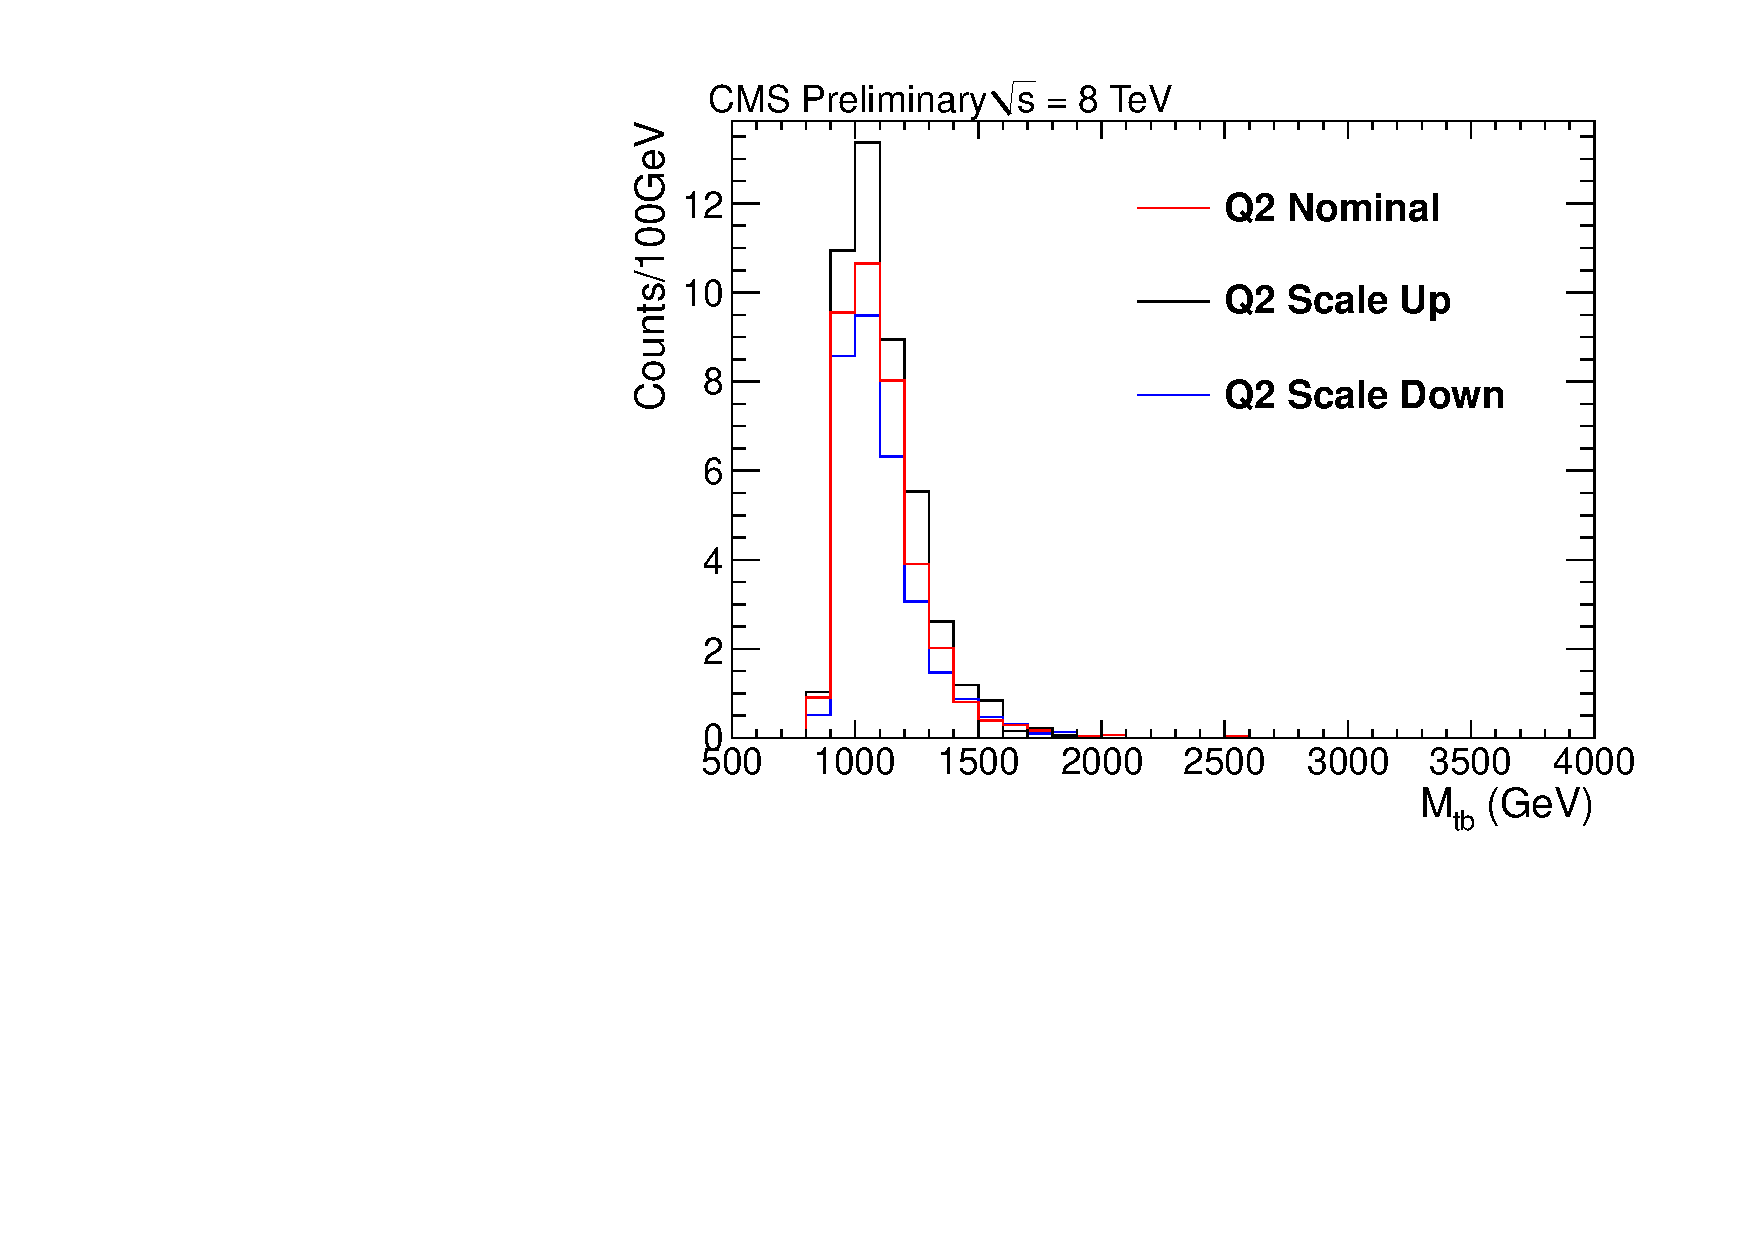
\includegraphics[width=0.7\textwidth]{AN-13-004/figs/TTbar_Q2Scale}
\caption{
$Q^2$ systematic variation for $\ttbar$ MC 
}
\label{figs:q2scale}
\end{center}
\end{figure}

\section{$\ttbar$ $\pt$ Re-weighting}
The uncertainty related to the $\pt$ re-weighting scheme presented in Section \ref{sec:ttptrw} is taken as the difference between the weighted and unweighted $\ttbar$ spectrum.
%However, this scheme has both a normalization and shape based effect.  Due to the fact that we extract the $\ttbar$ normalization uncertainty (see Section \ref{sec:ttbarsideband}), 
%we normalize the up and down systematic to the nominal $\pt$ re-weighting and use this in limit setting.
This uncertainty can be seen in figure \ref{figs:ptreweight}.  This is the dominant uncertainty for $\ttbar$. 

\begin{figure}[htcb]
\begin{center}
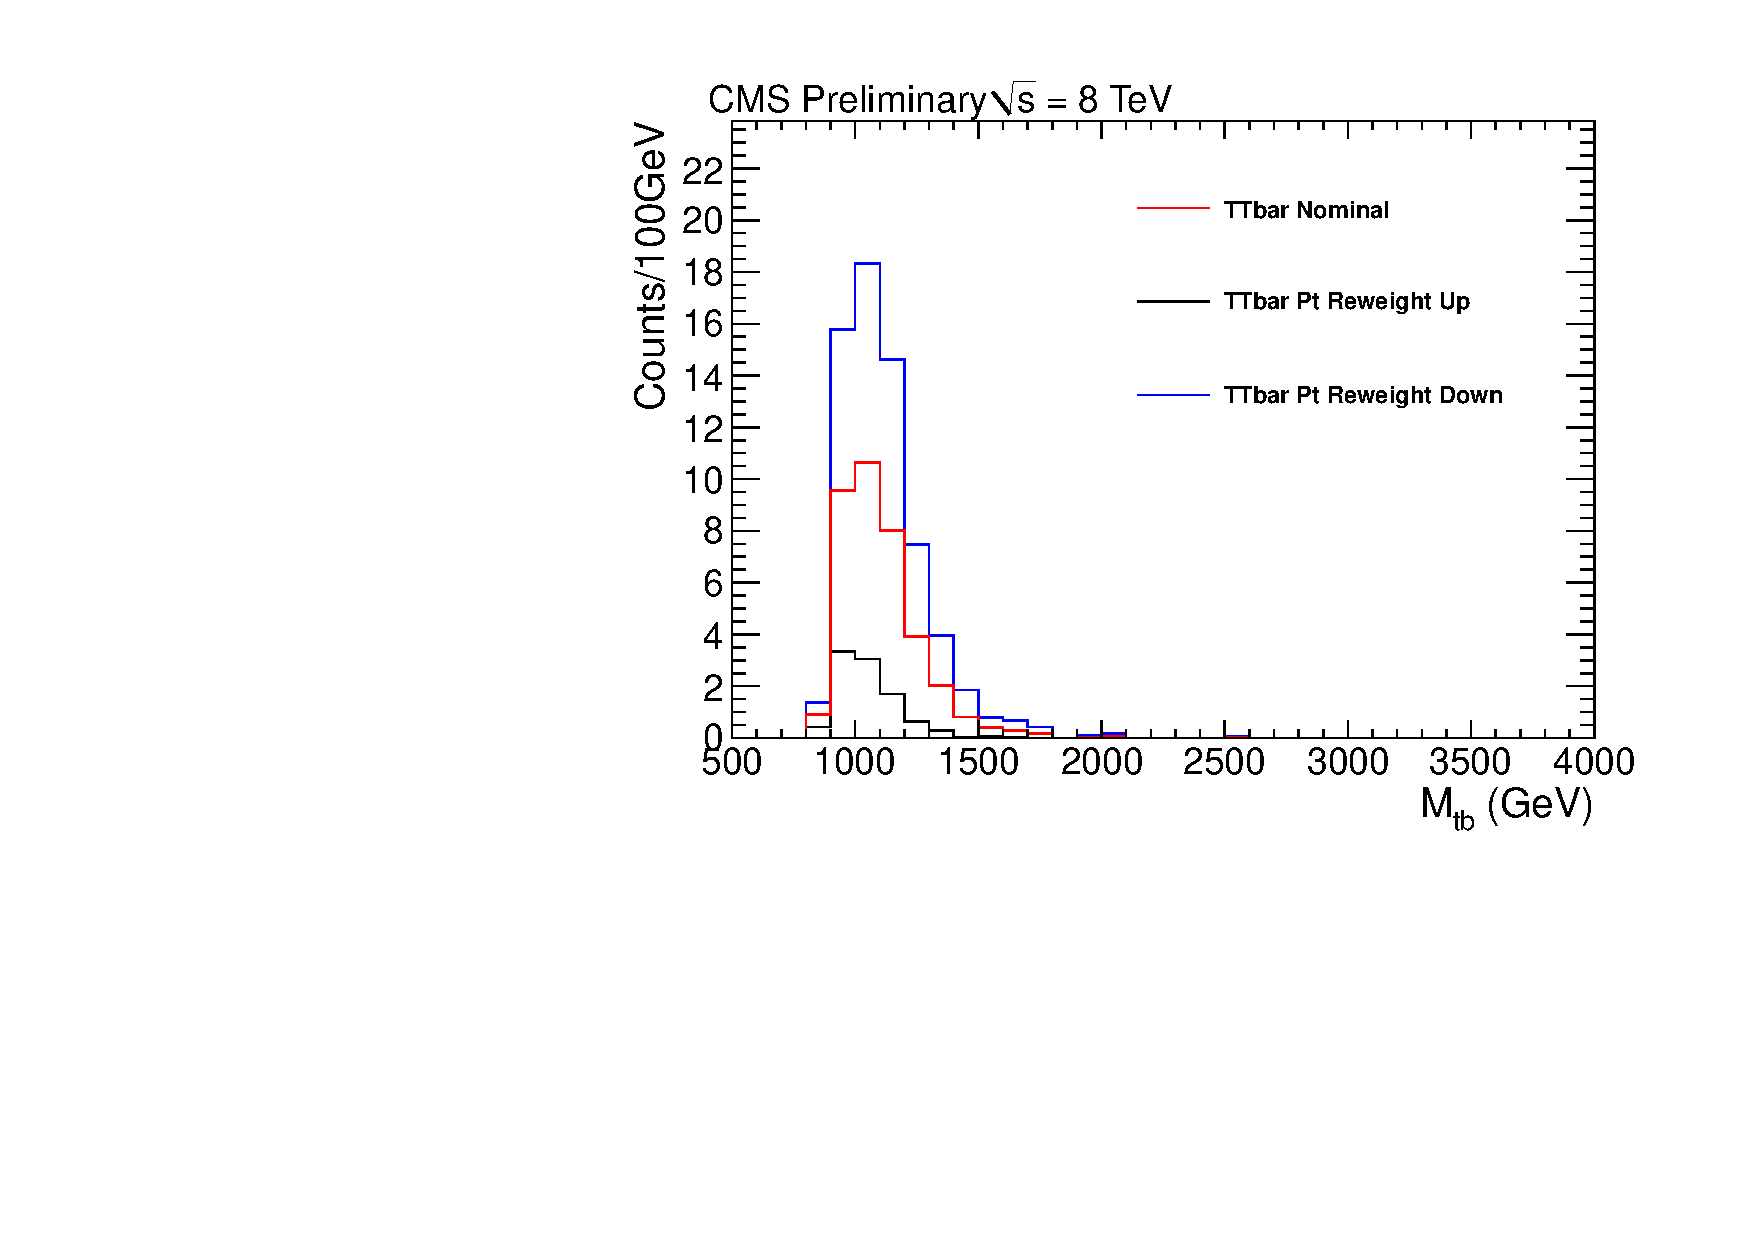
\includegraphics[width=0.7\textwidth]{AN-13-004/figs/TTbar_PTReweighting}
\caption{
$\pt$ re-weighting systematic variation for $\ttbar$ MC 
}
\label{figs:ptreweight}
\end{center}
\end{figure}

\section{Normalization Uncertainties}
As mentioned in Section \ref{sec:ttbarsideband}, the uncertainty due to the overall normalization scale factor used for $\ttbar$ is extracted from data and is $19\%$.   

We must apply a $13\%$ uncertainty on the top tagging scale factor described in Section \ref{sec:subjetSF} to signal MC events due to uncertainty in the difference in subjet efficiency from data to MC.

As mentioned in Section \ref{sec:btagging}, we add a $2\%$ uncertainty to the signal estimates from the AK5 vs. CA8 scale factor on b-tagging efficiency. 

We also include a $2.6\%$ uncertainty in the luminosity for the signal MC \cite{CMS-PAS-LUM-13-001}. 


\clearpage
\section{Uncertainties related to the QCD Background Estimate}
We use the result of the fit to the average b-tagging rate (see Chapter \ref{sec:backgroundEstimation}) to weight 
pre b-tagged events in order to create the QCD background estimate.  Uncertainties in
the fitting algorithm and statistical uncertainties in the sideband
are taken into account (see figure \ref{figs:tagrateetafit}).
Statistical uncertainties in the pre b tagged signal region are also
taken into account.

\subsection{Choice of the functional form for the average b-tagging rate}
\label{sec:choiceoffit}
The functional form used is a bifurcated polynomial.
However there is a systematic uncertainty associated with this choice.
The uncertainties due to this effect are taken into account by
studying alternative functional forms seen in figure
\ref{figs:BKGFITCOMP}.  The background estimation from these
alternative fits are seen in figure \ref{figs:BKGCOMP}.  The
uncertainty due to the choice of fit is taken as the Mean Squared
Error of these alternative backgrounds bin by bin and can be seen in
figure \ref{figs:BKGERR}.  


\subsection{Two-dimensional  vs. three-dimensional parameterization of the average b-tagging rate}
\label{sec:paramerrors1}
Additionally, we place an uncertainty on the inability of the
background estimate to capture all kinematic correlations through the
parameterization of the average b-tagging rate in $\pt$ and $\eta$.
This uncertainty is calculated by investigating a parameterization in
$\pt$ $\eta$ and $\mathrm{M_{tb}}$.  We define $P_i$ as the average b-tagging
rate described in Chapter \ref{sec:backgroundEstimation} in one
$\eta$ bin and $P_{ij}$ as the average b-tagging rate if parameterized
with $\mathrm{M_{tb}}$ as well.  $P_{ij}$ can be seen in
figure \ref{figs:sb2deta}.  Each bin in $P_i$ can be thought of as a
column average over all $\mathrm{M_{tb}}$ bins per $\pt$ bin.  If $P_{ij}$ a
function of $\mathrm{M_{tb}}$ (index $j$) is not constant, then averaging over
$P_{ij}$ over $j$ while projecting onto $\mathrm{M_{tb}}$ axis to obtain the
QCD background estimate can result in a bias.  For more in-depth
discussion on this effect, please see Section \ref{sec:qcdpunc}.

We assess the approximate size of the uncertainty due to our choice of
parameterization by explicitly comparing the three-dimensional and
two-dimensional background estimates in the sideband.  Using these two
parameterizations, the uncertainty in the $\mathrm{M_{tb}}$ distribution due to
parameterization is approximately $\displaystyle\sum\limits_{j=0}^n
m_{ij}$($P_{ij}-P_i$) where $m_{ij}$ refers to the number of pretag
events for a bin in $\pt$ and $\mathrm{M_{tb}}$.  Fig. \ref{figs:PARAMERROR}
shows the uncertainty due to this effect. These uncertainties are
taken in quadrature to produce an overall uncertainty in the data
derived background estimate that is applied in a shape based manner in
the limit-setting macro.

\begin{sidewaystable}
\begin{center}
\bf{Rate Effects of Systematic Uncertainties}\\
\scalebox{0.5}{
\begin{tabular}{|c||c|c|c|c|c|c|c|c|c|c|c|}
\hline
\bf{Sample} & \bf{CA btag SF}  & \bf{QCD total} & \bf{b-tagging}  & \bf{JES}  & \bf{Lumi}  & \bf{$\pt$ Reweight} & \bf{JER}  & \bf{$Q^2$}  & \bf{Subjet SF}  & \bf{Trigger}  & \bf{$\ttbar$ Norm} \\
\hline
qcd & --- & +9.05,-8.94 & --- & --- & --- & --- & --- & --- & --- & --- & ---\\
\hline
ttbar & --- & --- & +4.49,-4.49 & -0.42,+0.49 & +16.49,-15.27 & --- & +21.77,-14.96 & -74.04,+77.89 & --- & +0.30,-0.30 & +19.00,-15.97\\
\hline
1300 & +2.00,-1.96 & --- & +6.08,-6.08 & -0.27,+0.29 & +2.06,-3.85 & +2.60,-2.53 & --- & --- & +12.50,-11.11 & +0.06,-0.06 & ---\\
\hline
1500 & +2.00,-1.96 & --- & +6.48,-6.48 & -0.03,+0.17 & -0.29,-0.19 & +2.60,-2.53 & --- & --- & +12.50,-11.11 & +0.02,-0.02 & ---\\
\hline
1700 & +2.00,-1.96 & --- & +6.94,-6.94 & -0.02,+0.12 & -1.27,+1.17 & +2.60,-2.53 & --- & --- & +12.50,-11.11 & +0.01,-0.01 & ---\\
\hline
1900 & +2.00,-1.96 & --- & +8.12,-8.12 & -0.08,+0.02 & -1.76,+1.78 & +2.60,-2.53 & --- & --- & +12.50,-11.11 & +0.01,-0.01 & ---\\
\hline
2100 & +2.00,-1.96 & --- & +9.39,-9.39 & +0.06,-0.05 & -1.81,+1.61 & +2.60,-2.53 & --- & --- & +12.50,-11.11 & +0.01,-0.01 & ---\\
\hline
2300 & +2.00,-1.96 & --- & +10.01,-10.01 & +0.02,+0.09 & -1.76,+1.24 & +2.60,-2.53 & --- & --- & +12.50,-11.11 & +0.02,-0.02 & ---\\
\hline
2700 & +2.00,-1.96 & --- & +9.49,-9.49 & -0.25,+0.08 & -0.33,+0.47 & +2.60,-2.53 & --- & --- & +12.50,-11.11 & +0.04,-0.04 & ---\\
\hline
\end{tabular}
}
\end{center}
\caption{Rate effects of the systematic uncertainties as extracted from Theta.  The numbers listed under sample specify $\wpr_R$ signal MC mass.}
\label{table:nuisance}
\end{sidewaystable}


\begin{figure}[htcb]
\begin{center}
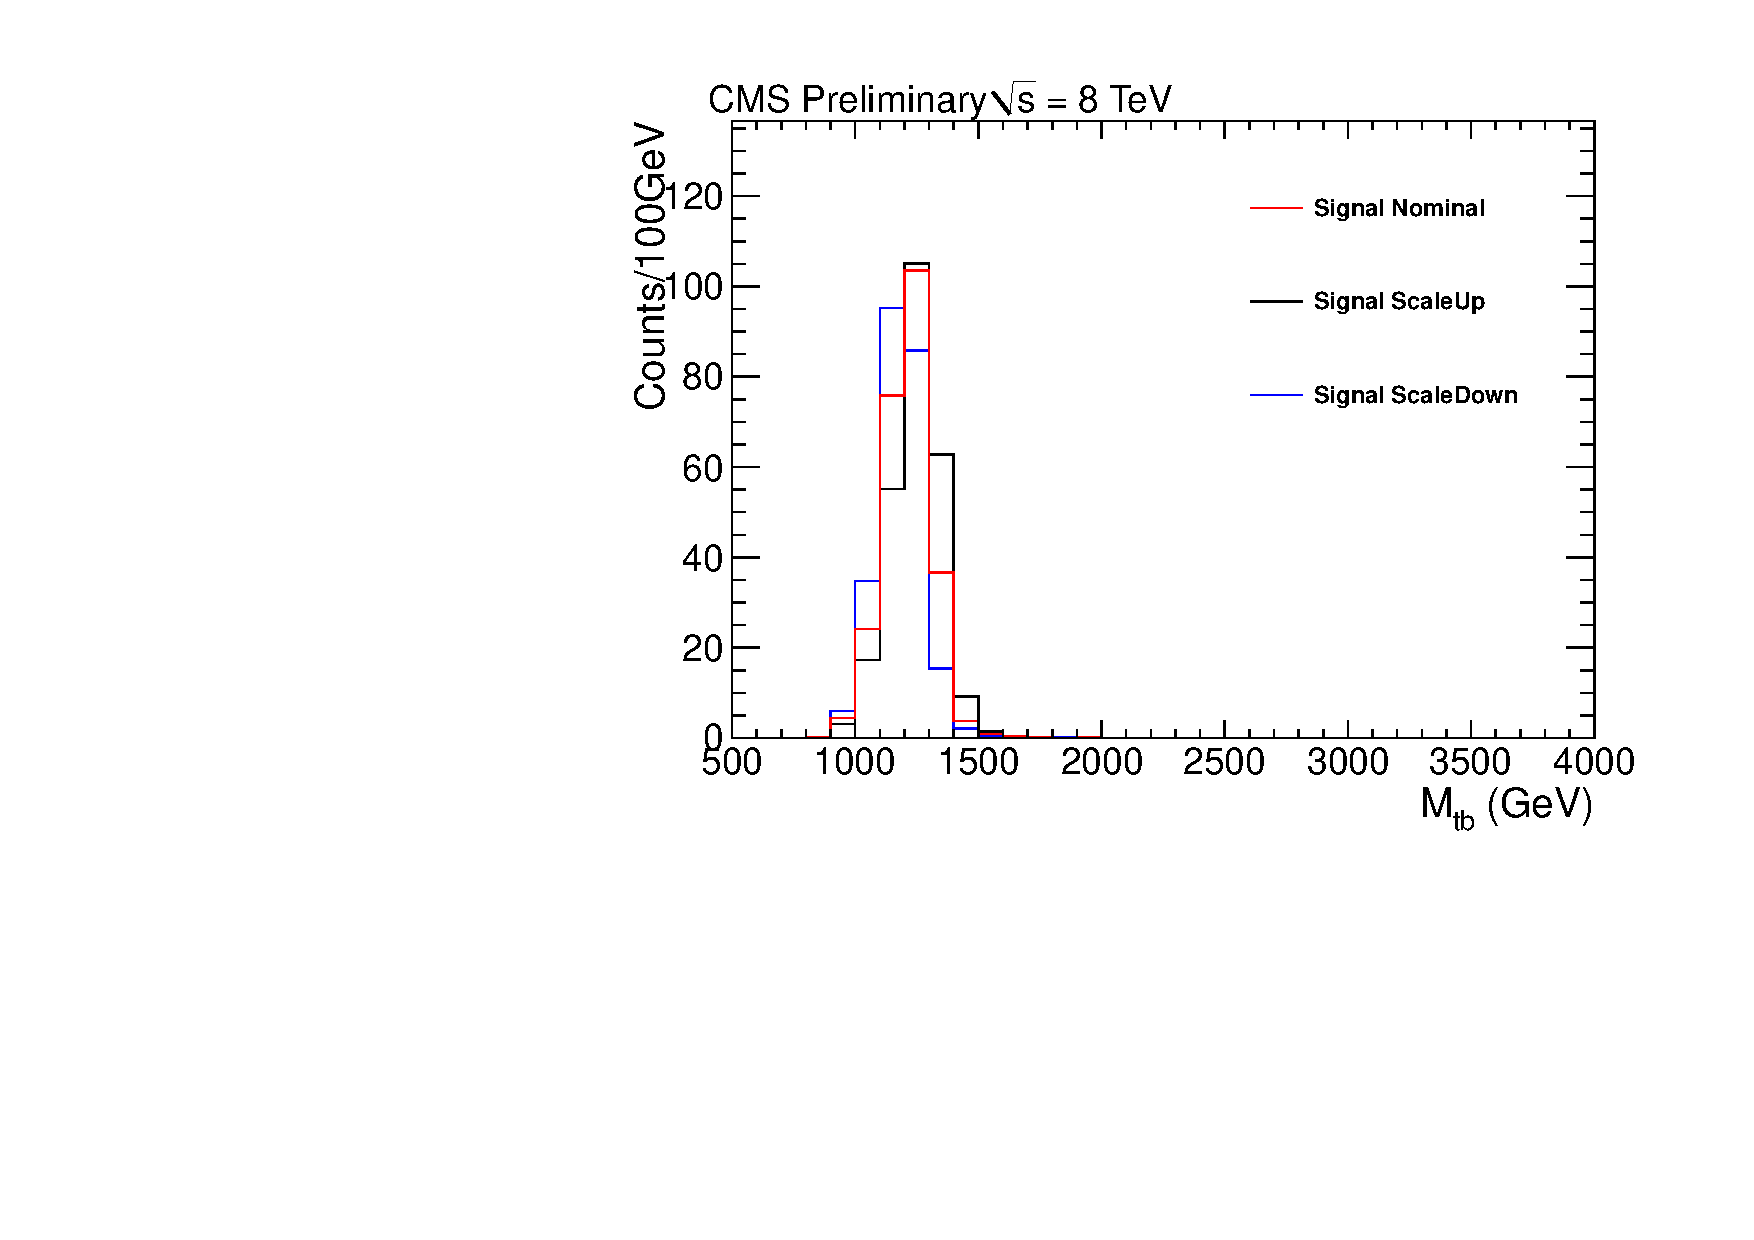
\includegraphics[width=0.4\textwidth]{AN-13-004/figs/Signal_M1300_PtScaling}
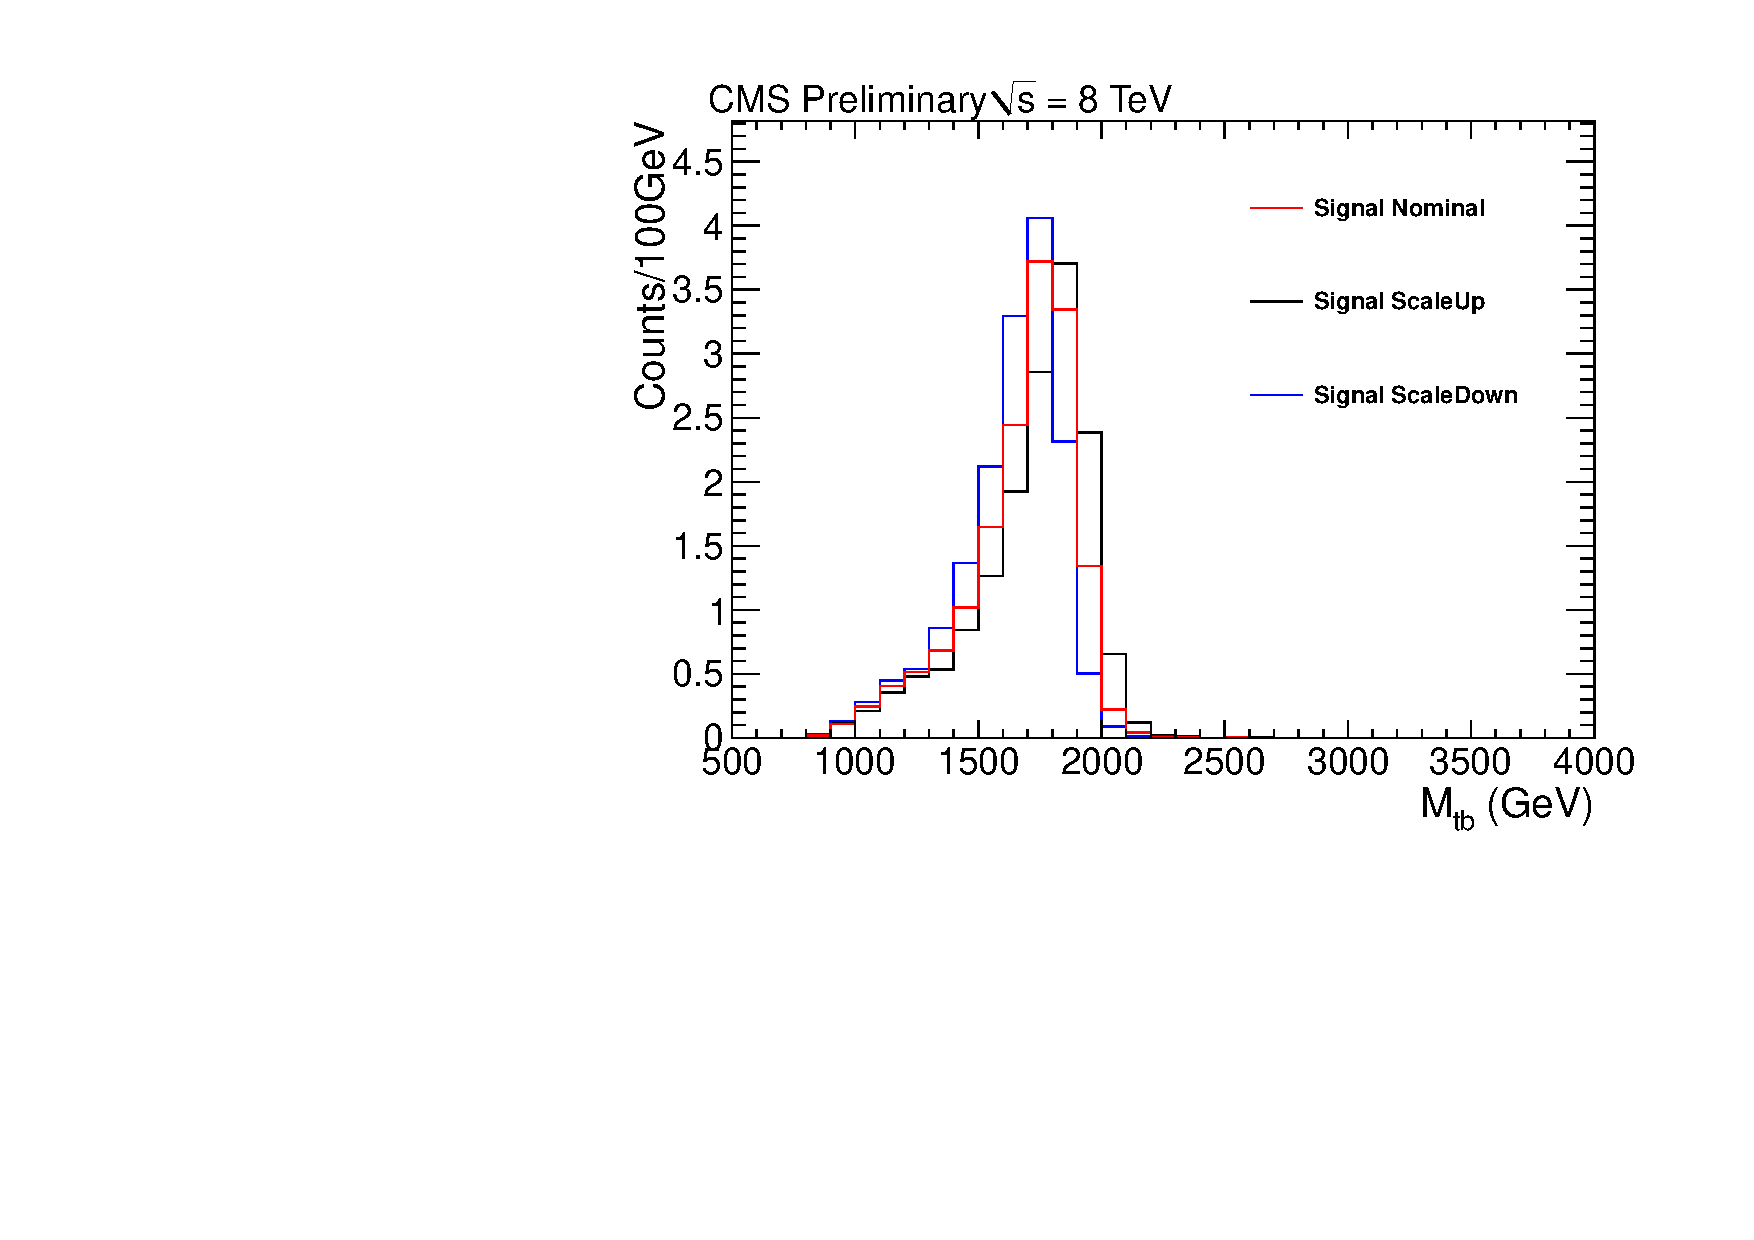
\includegraphics[width=0.4\textwidth]{AN-13-004/figs/Signal_M1900_PtScaling}
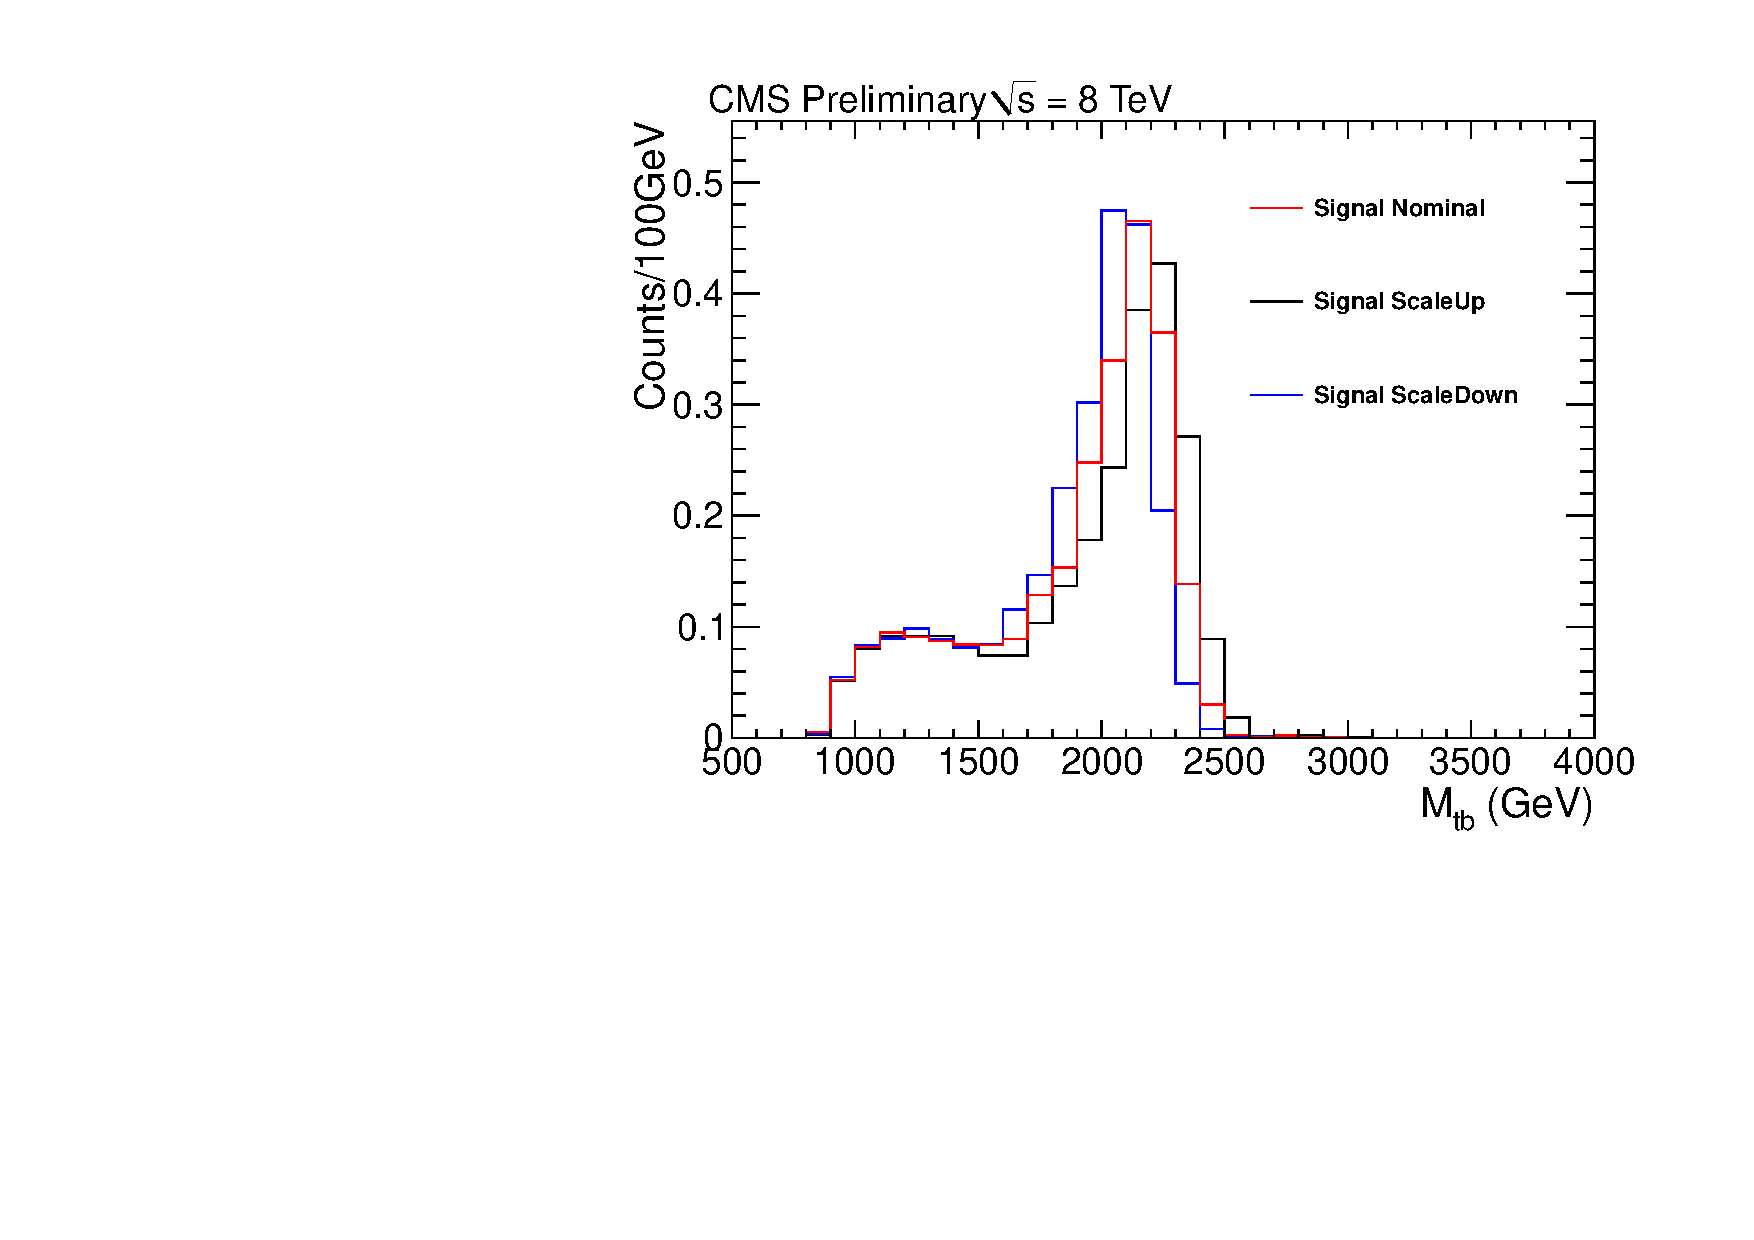
\includegraphics[width=0.4\textwidth]{AN-13-004/figs/Signal_M2300_PtScaling}
\caption{
Jet Energy Scale systematic variation for Right-handed $\wpr$ MC at the following mass points
(a) $M_{\wpr}$ = 1300$~\GeV$ 
(b) $M_{\wpr}$ = 1900$~\GeV$
(c) $M_{\wpr}$ = 2300$~\GeV$ 
}
\label{figs:signalJES}
\end{center}
\end{figure}

\begin{figure}[htcb]
\begin{center}
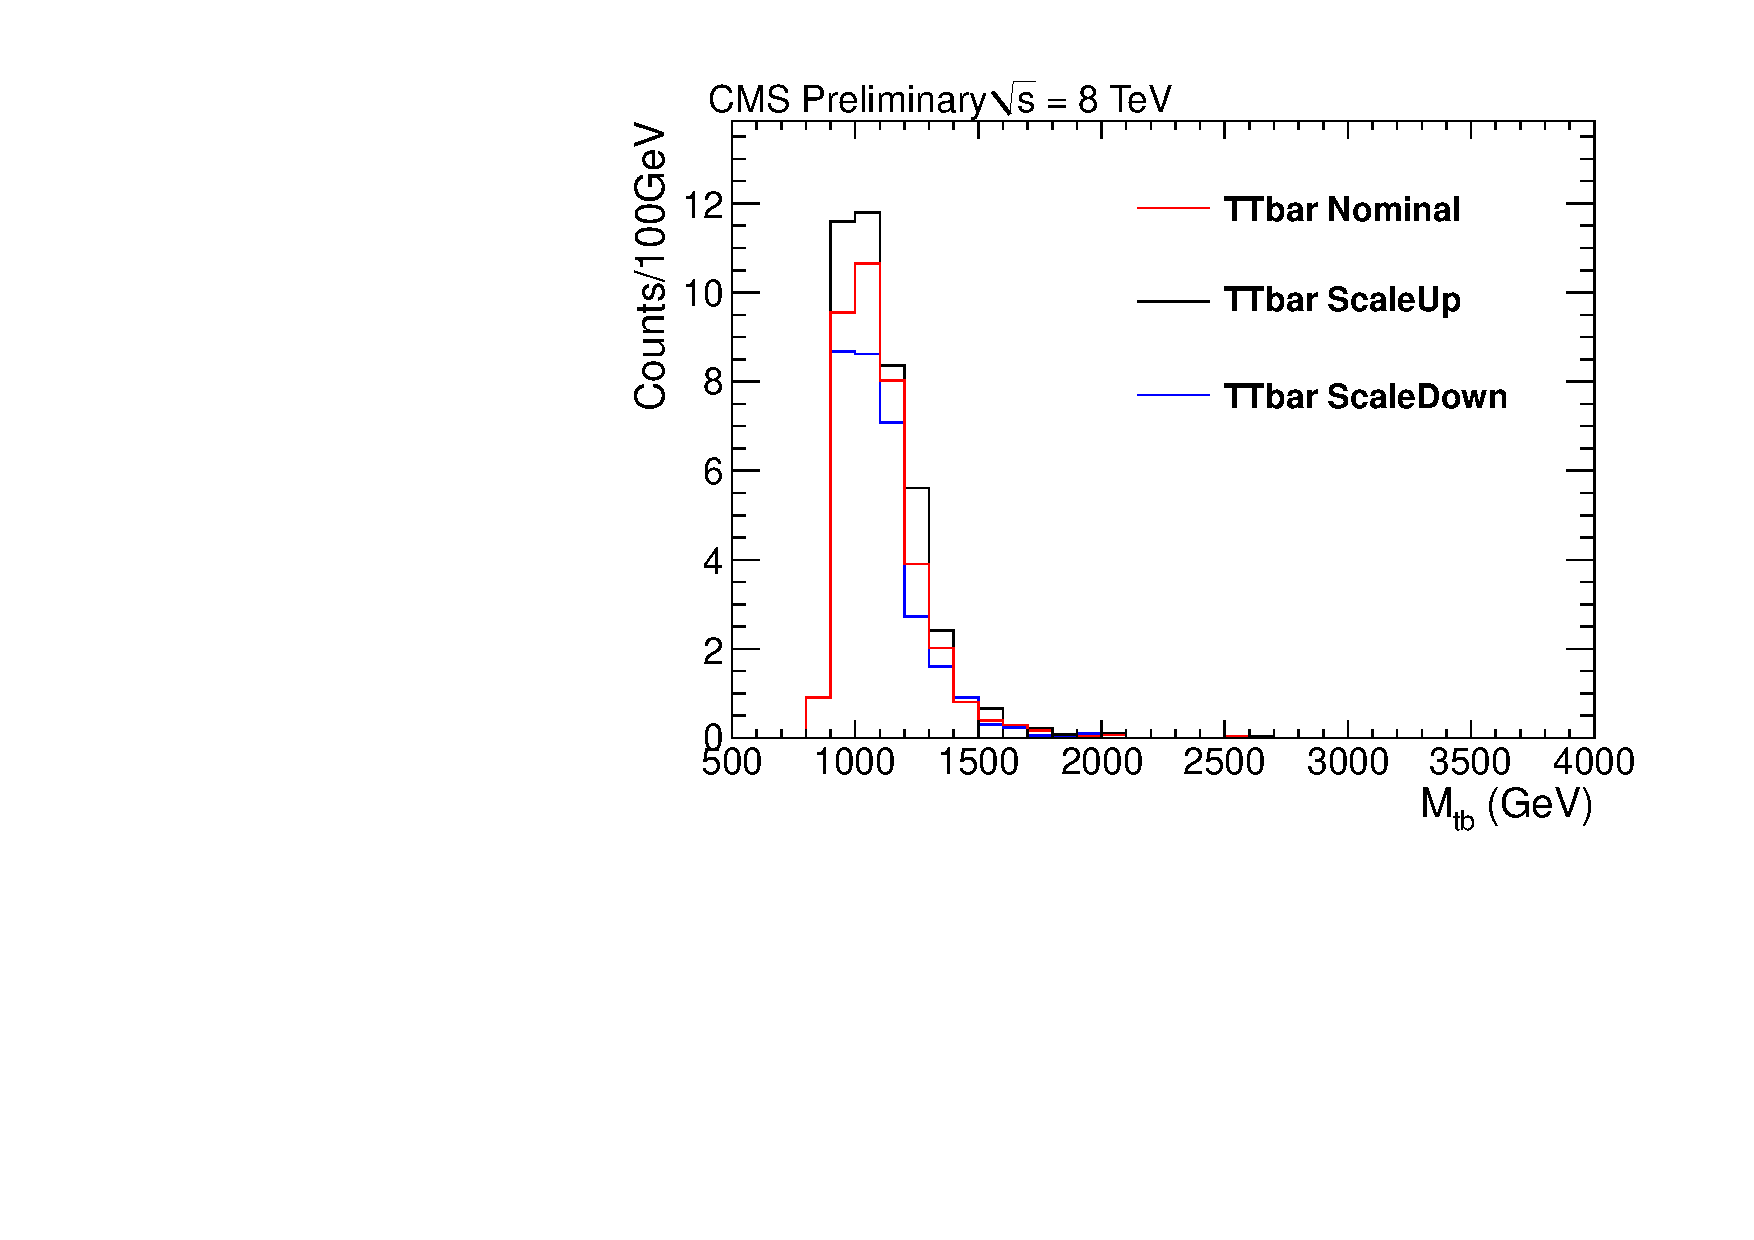
\includegraphics[width=0.7\textwidth]{AN-13-004/figs/TTbar_PtScaling}
\caption{Jet Energy Scale systematic variation for $\ttbar$ MC}
\label{figs:ttbarJES}
\end{center}
\end{figure}

\begin{figure}[htcb]
\begin{center}
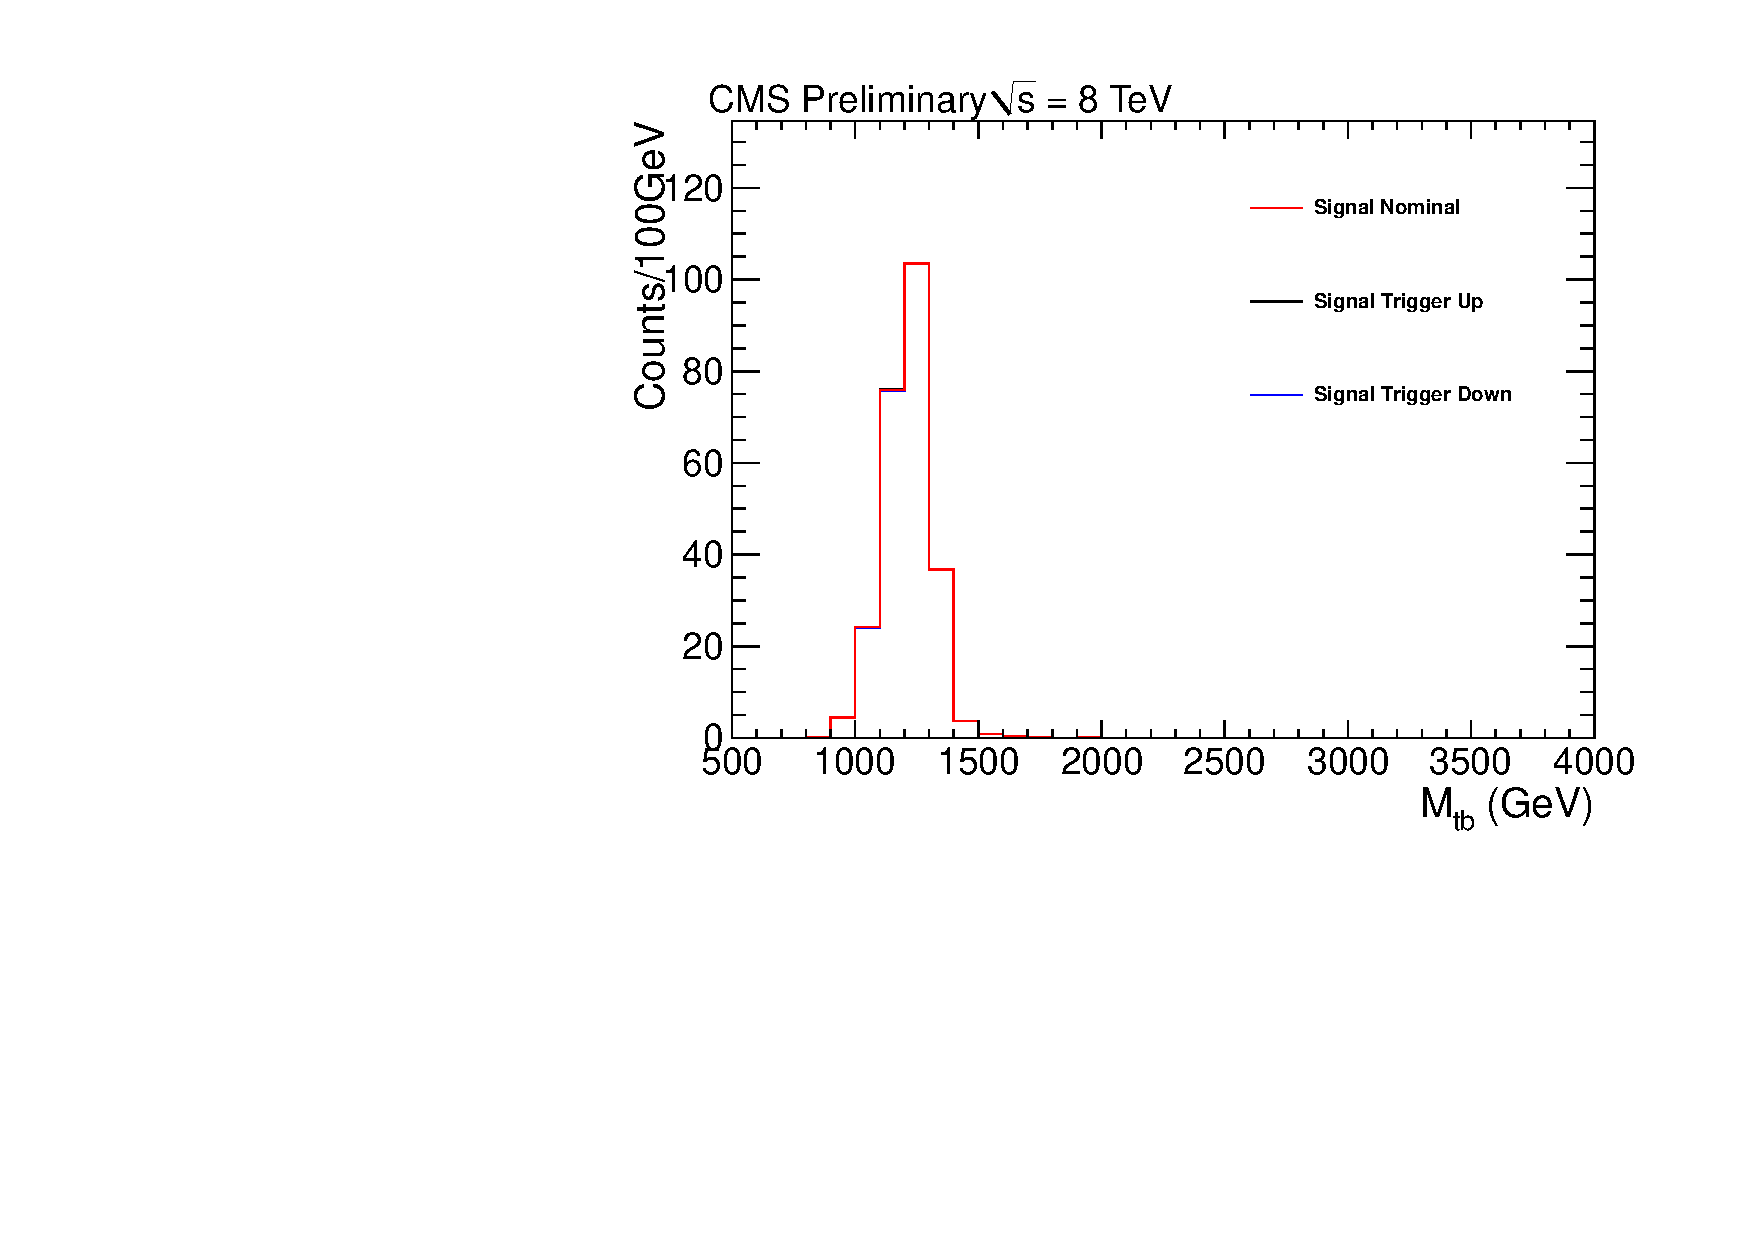
\includegraphics[width=0.45\textwidth]{AN-13-004/figs/Signal_M1300_TriggerWeighting}
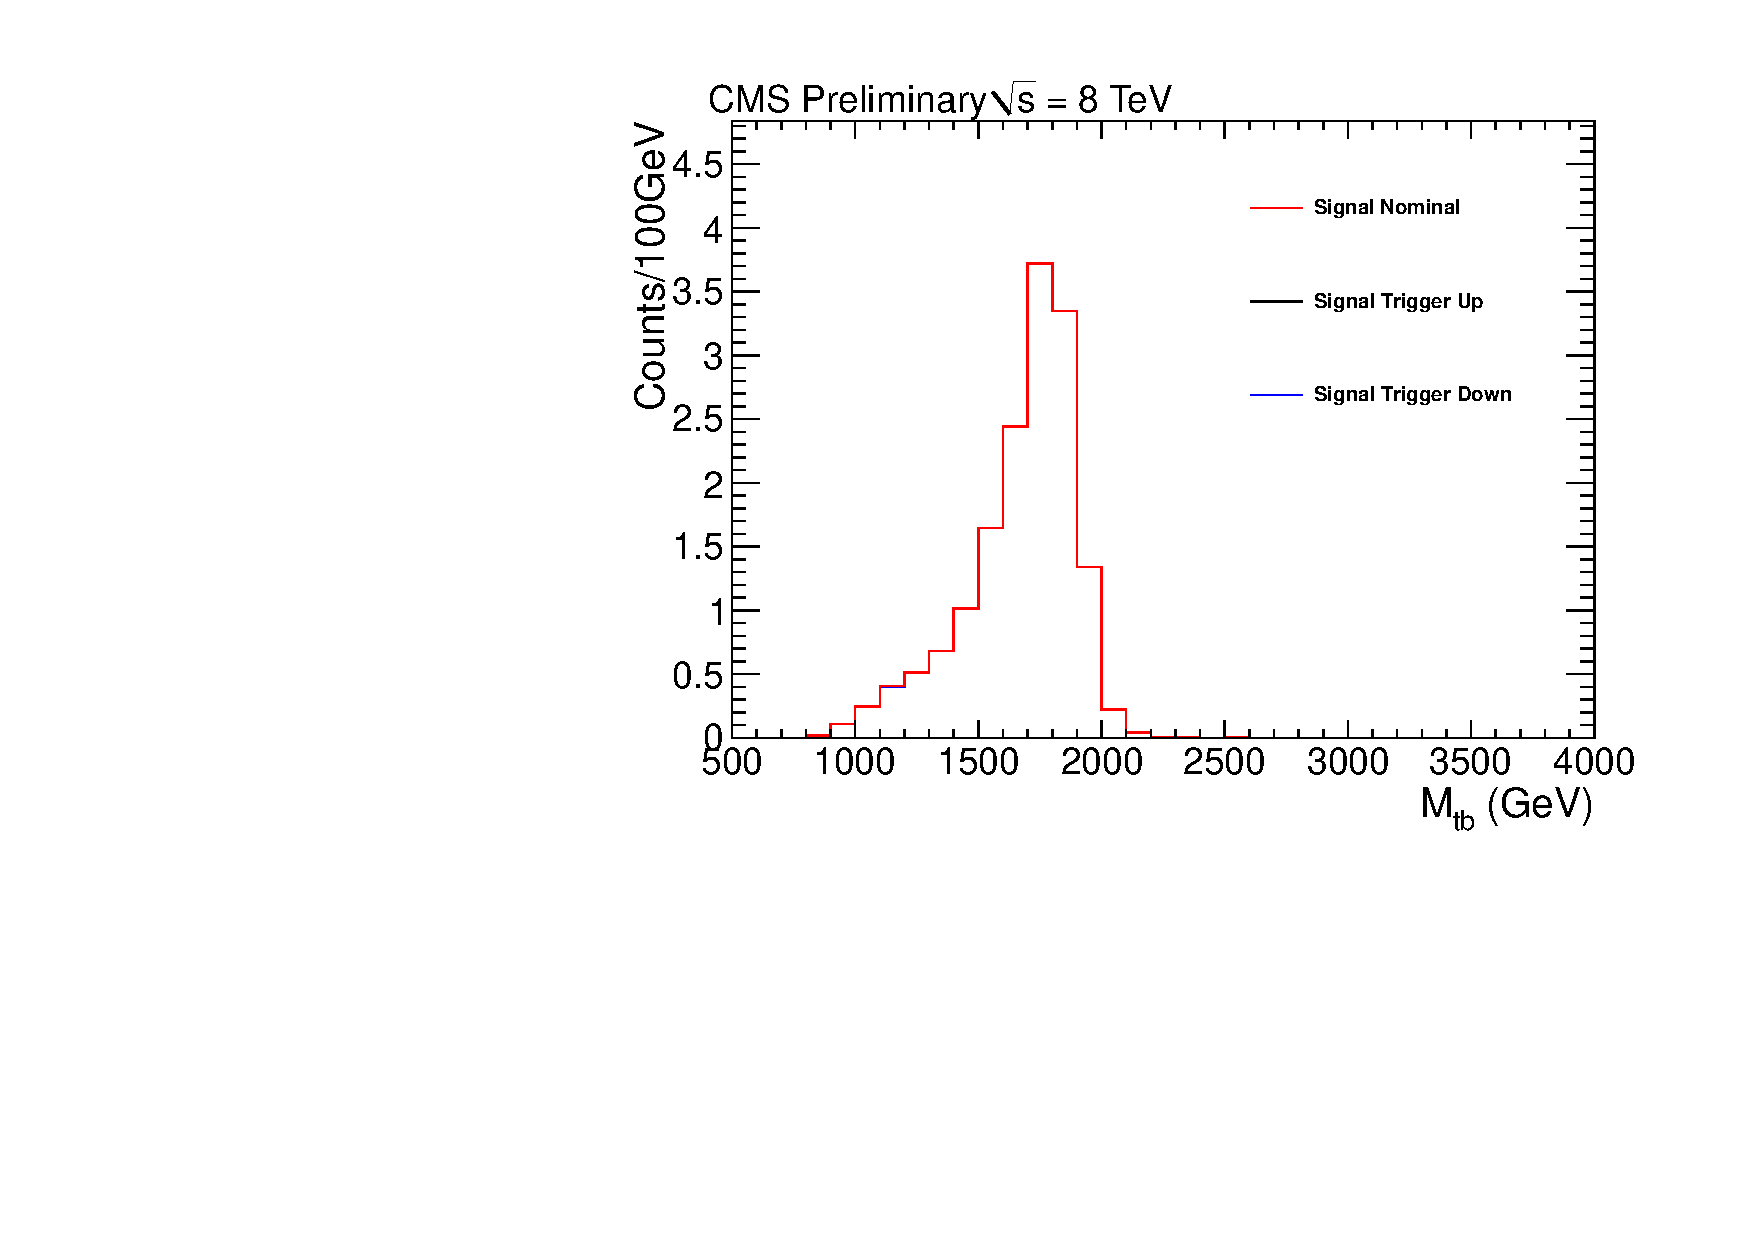
\includegraphics[width=0.45\textwidth]{AN-13-004/figs/Signal_M1900_TriggerWeighting}
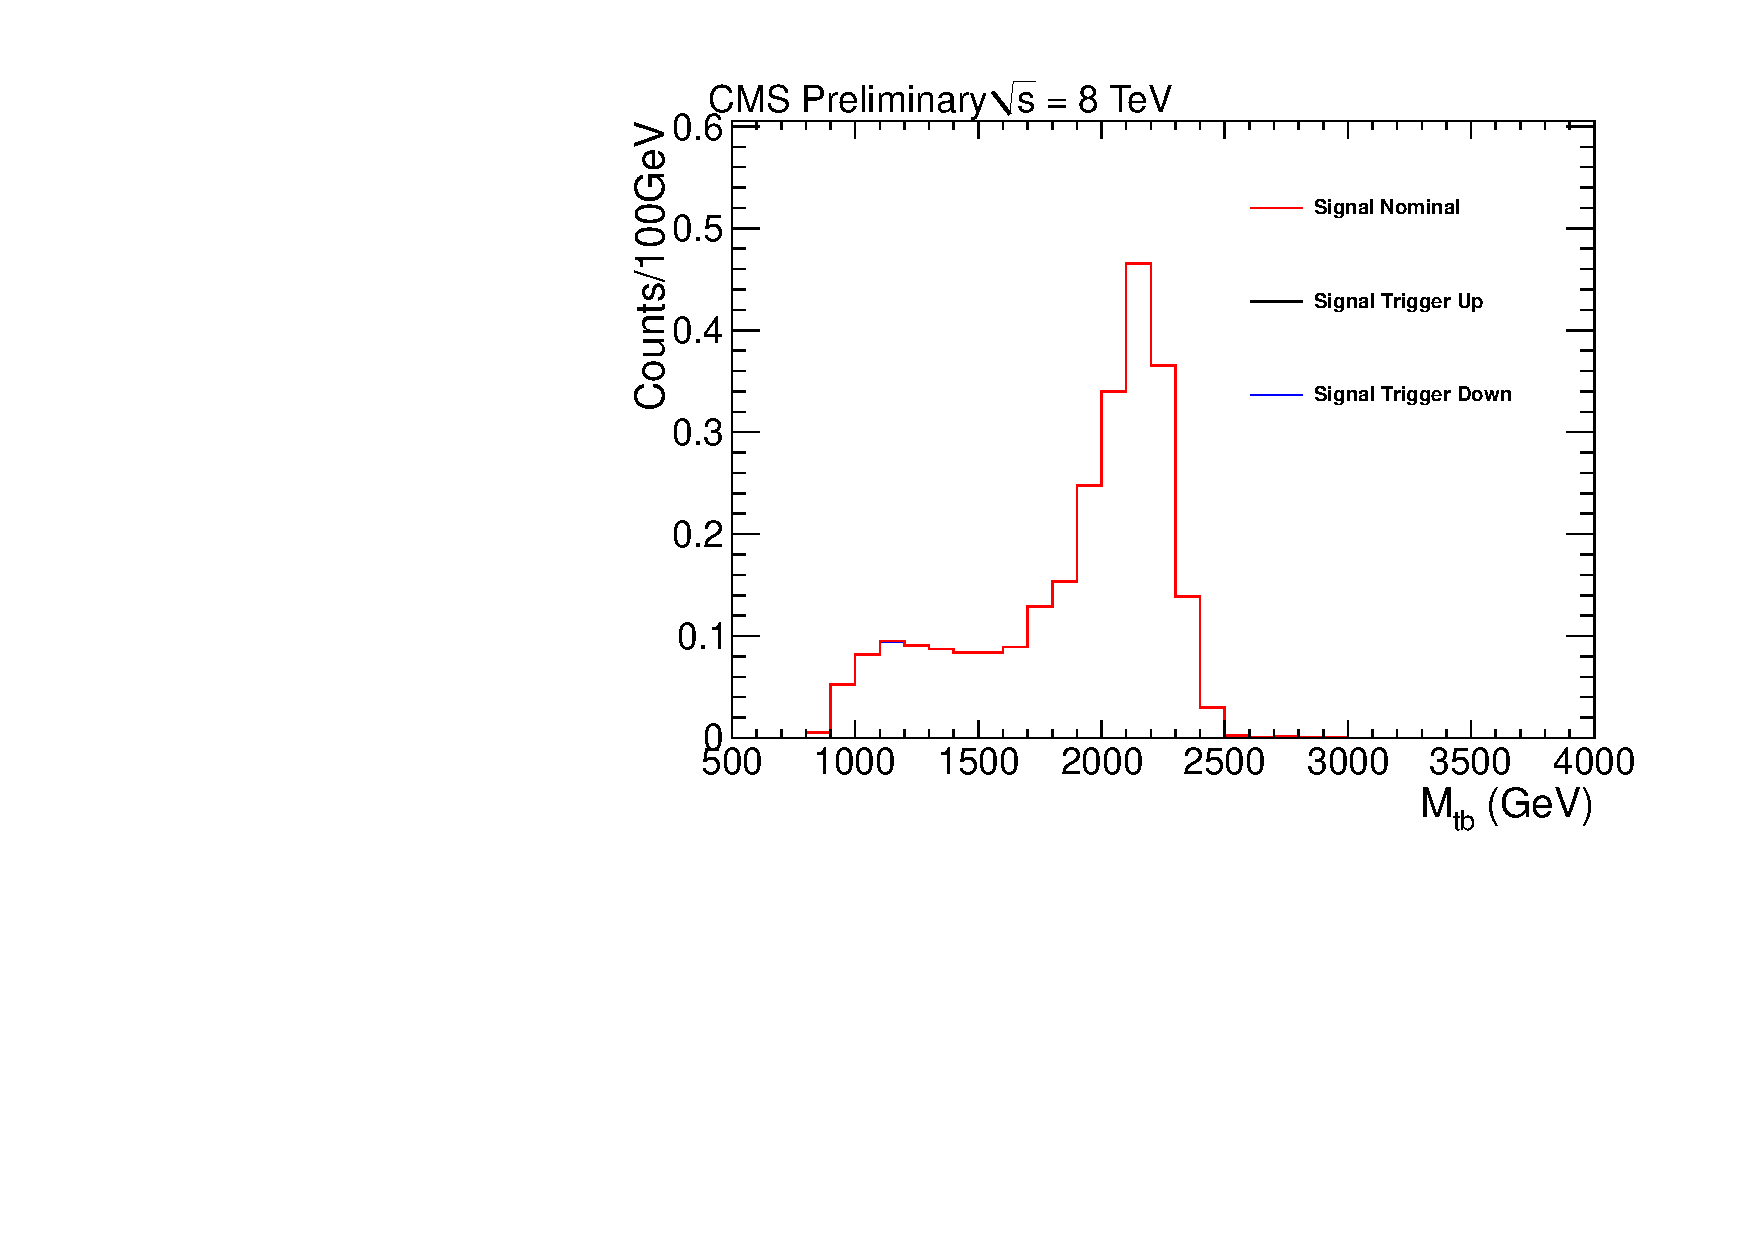
\includegraphics[width=0.45\textwidth]{AN-13-004/figs/Signal_M2300_TriggerWeighting}
\caption{
Trigger Weighting systematic variation for Right-handed $\wpr$ MC at the following mass points
(a) $M_\wpr$ = 1300$~\GeV$ 
(b) $M_\wpr$ = 1900$~\GeV$
(c) $M_\wpr$ = 2300$~\GeV$ 
}
\label{figs:signaltrig}
\end{center}
\end{figure}

\begin{figure}[htcb]
\begin{center}
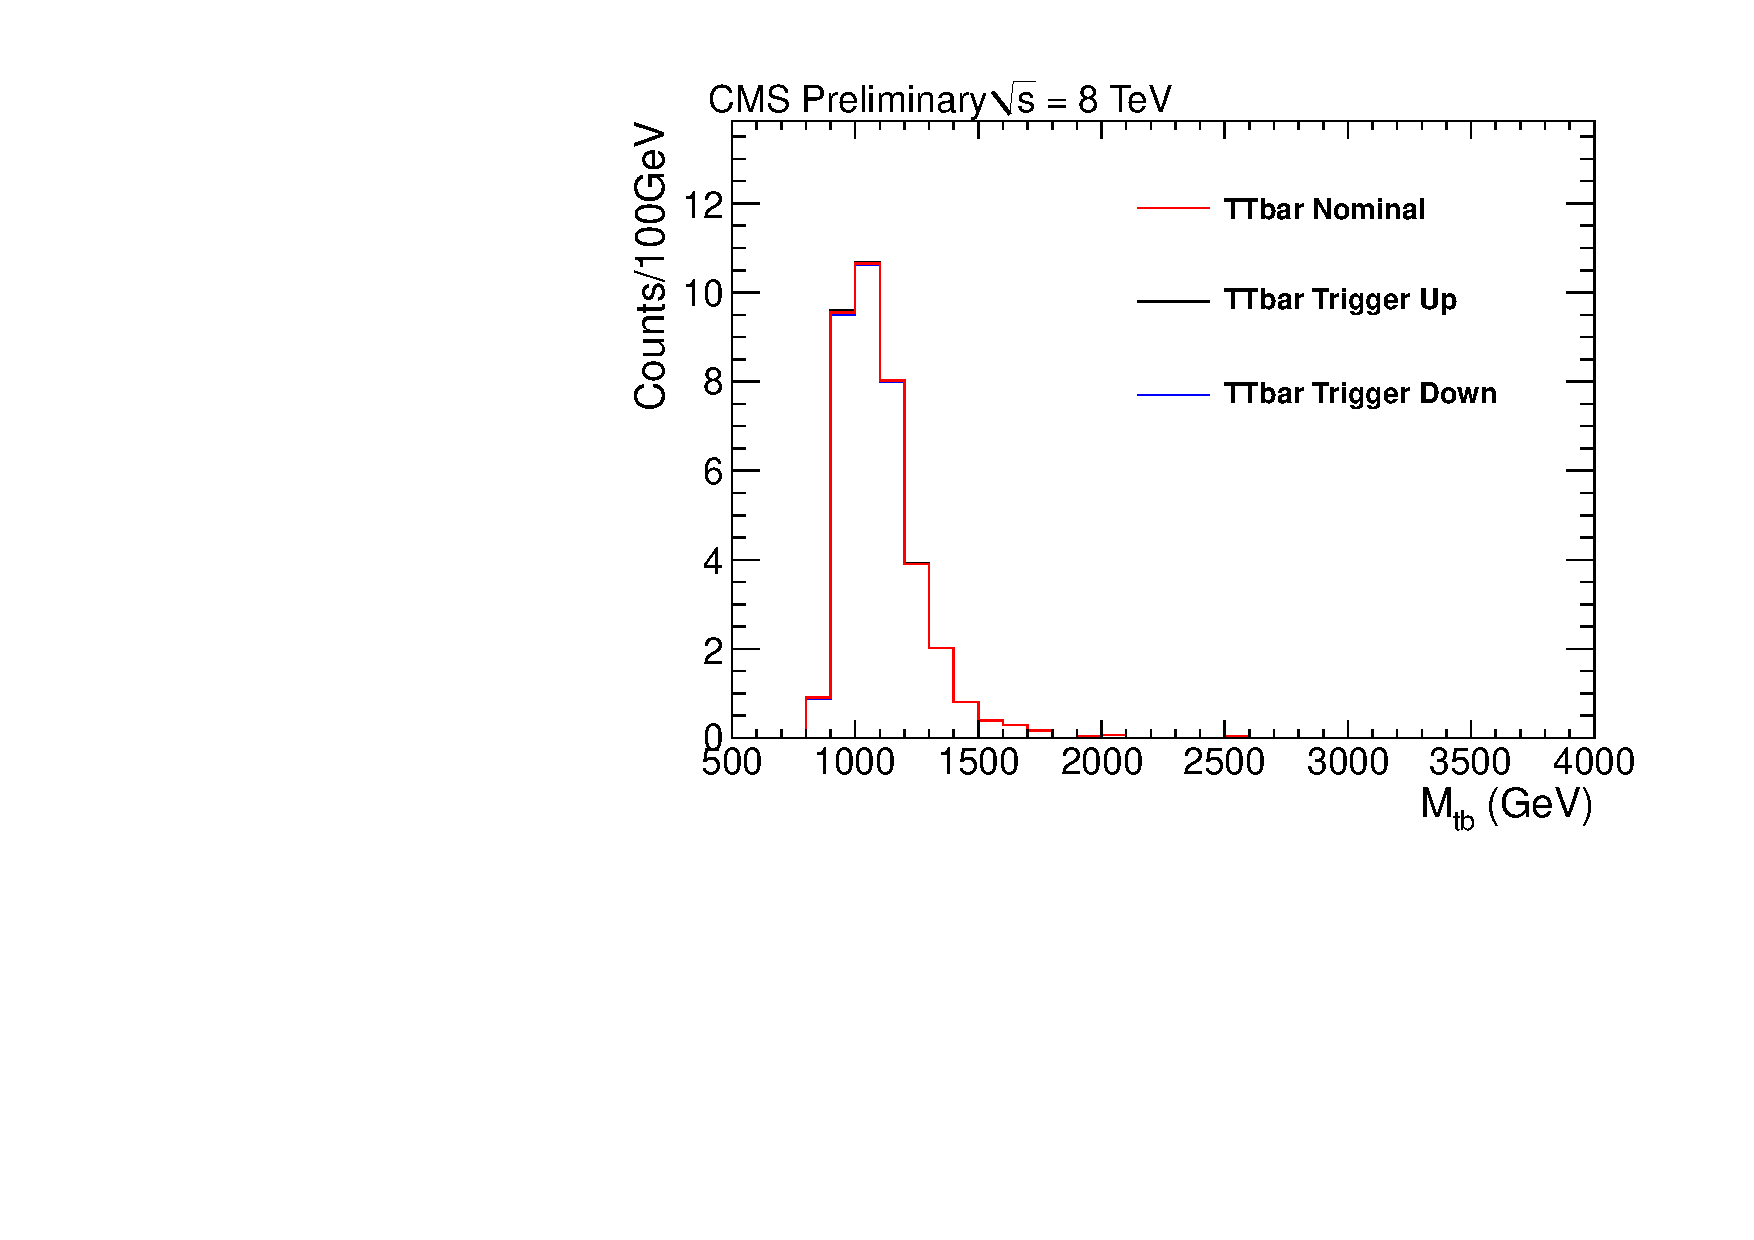
\includegraphics[width=0.7\textwidth]{AN-13-004/figs/TTbar_TriggerWeighting}
\caption{Trigger Weighting systematic variation for $\ttbar$ MC}
\label{figs:ttbartrig}
\end{center}
\end{figure}


\begin{figure}[htcb]
\begin{center}
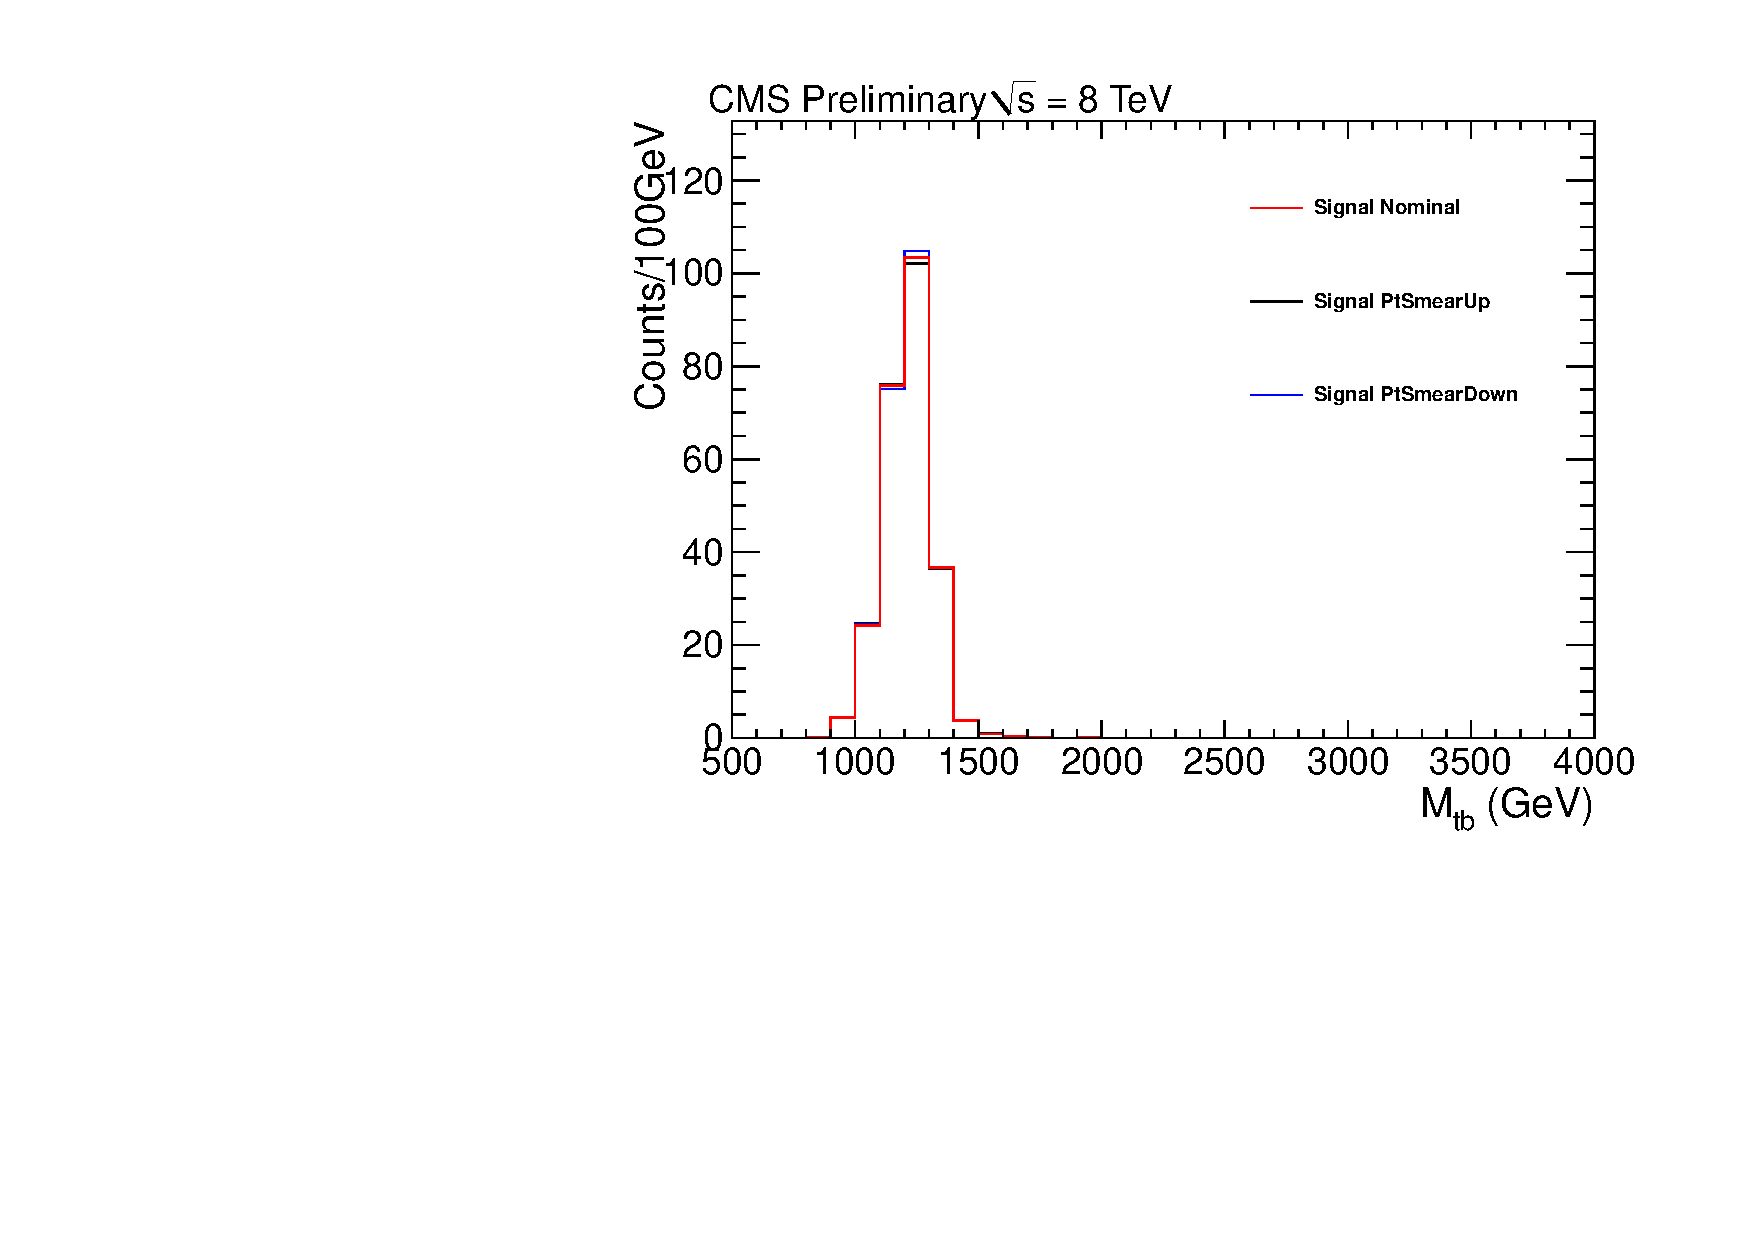
\includegraphics[width=0.45\textwidth]{AN-13-004/figs/Signal_M1300_PtSmearing}
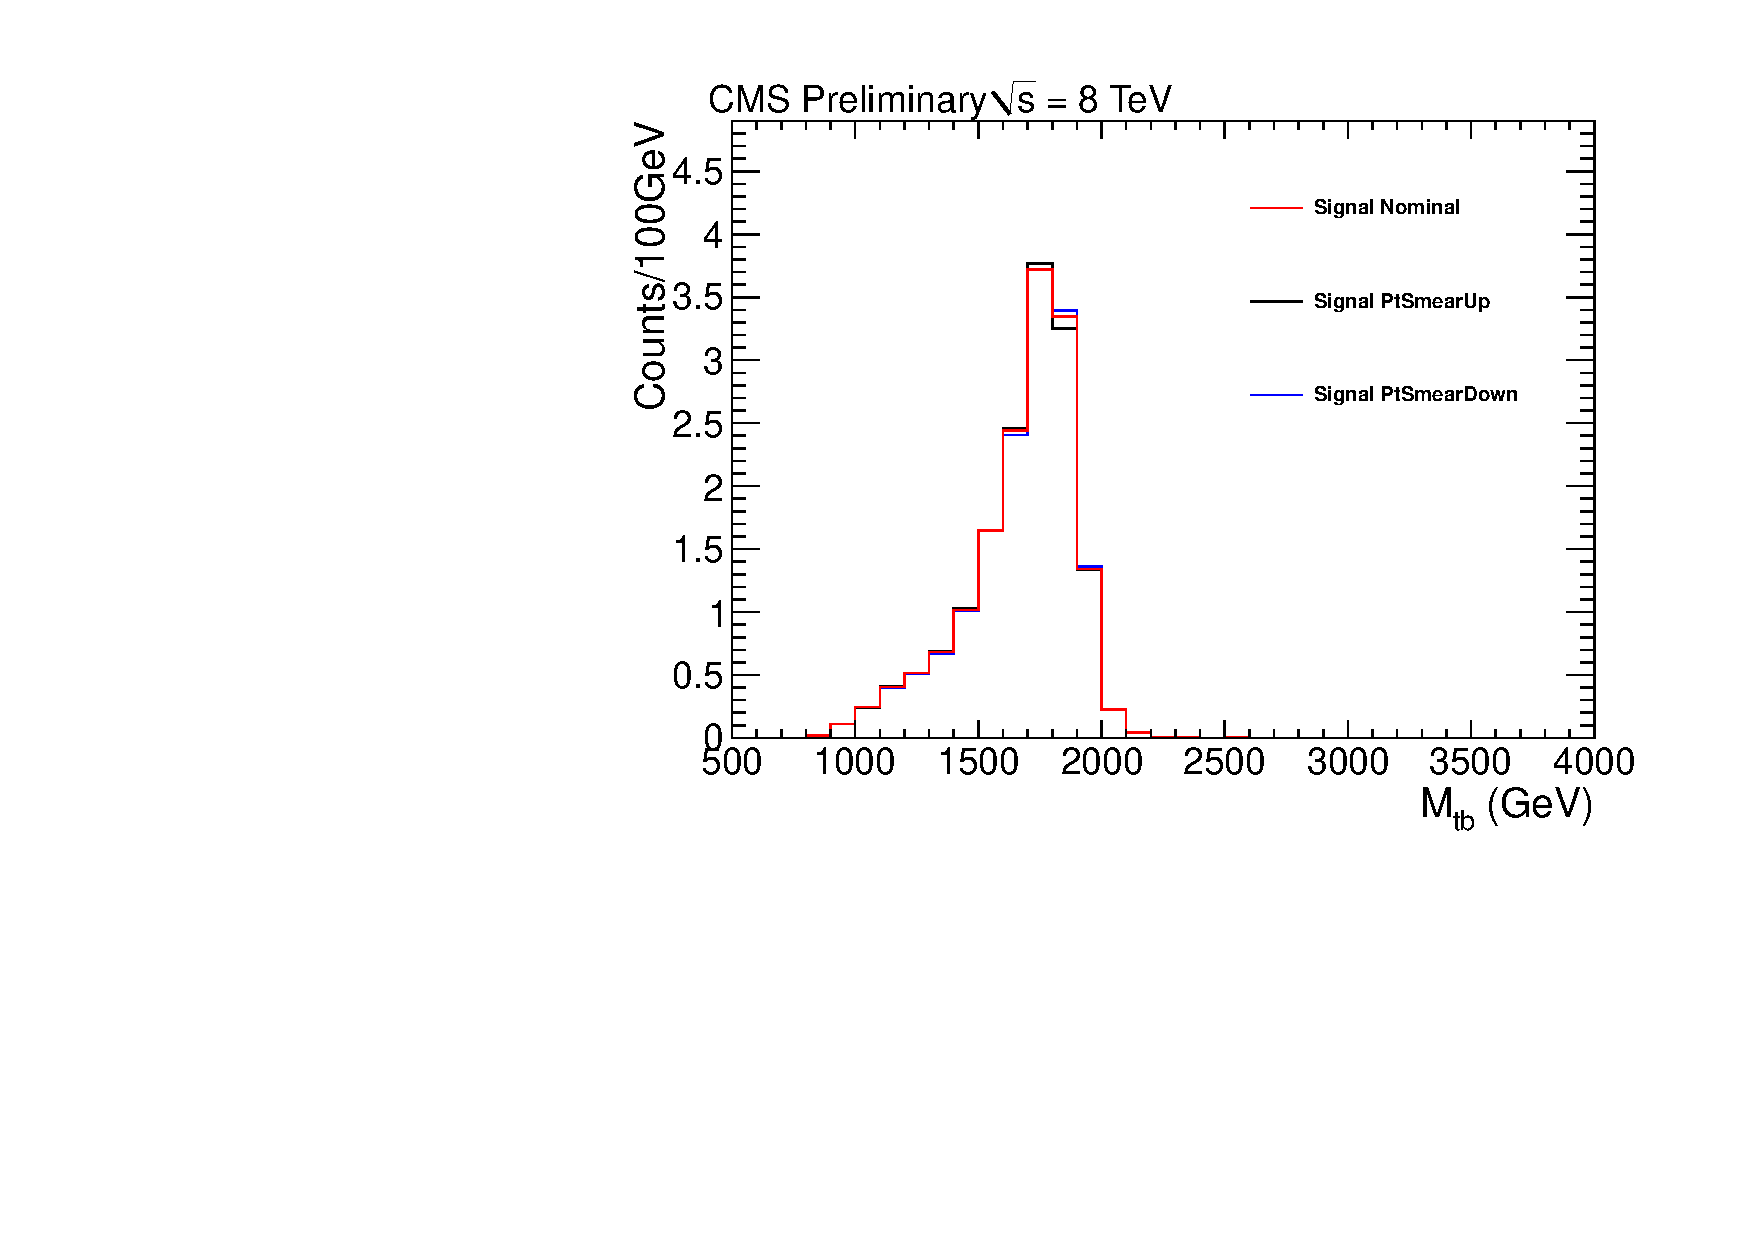
\includegraphics[width=0.45\textwidth]{AN-13-004/figs/Signal_M1900_PtSmearing}
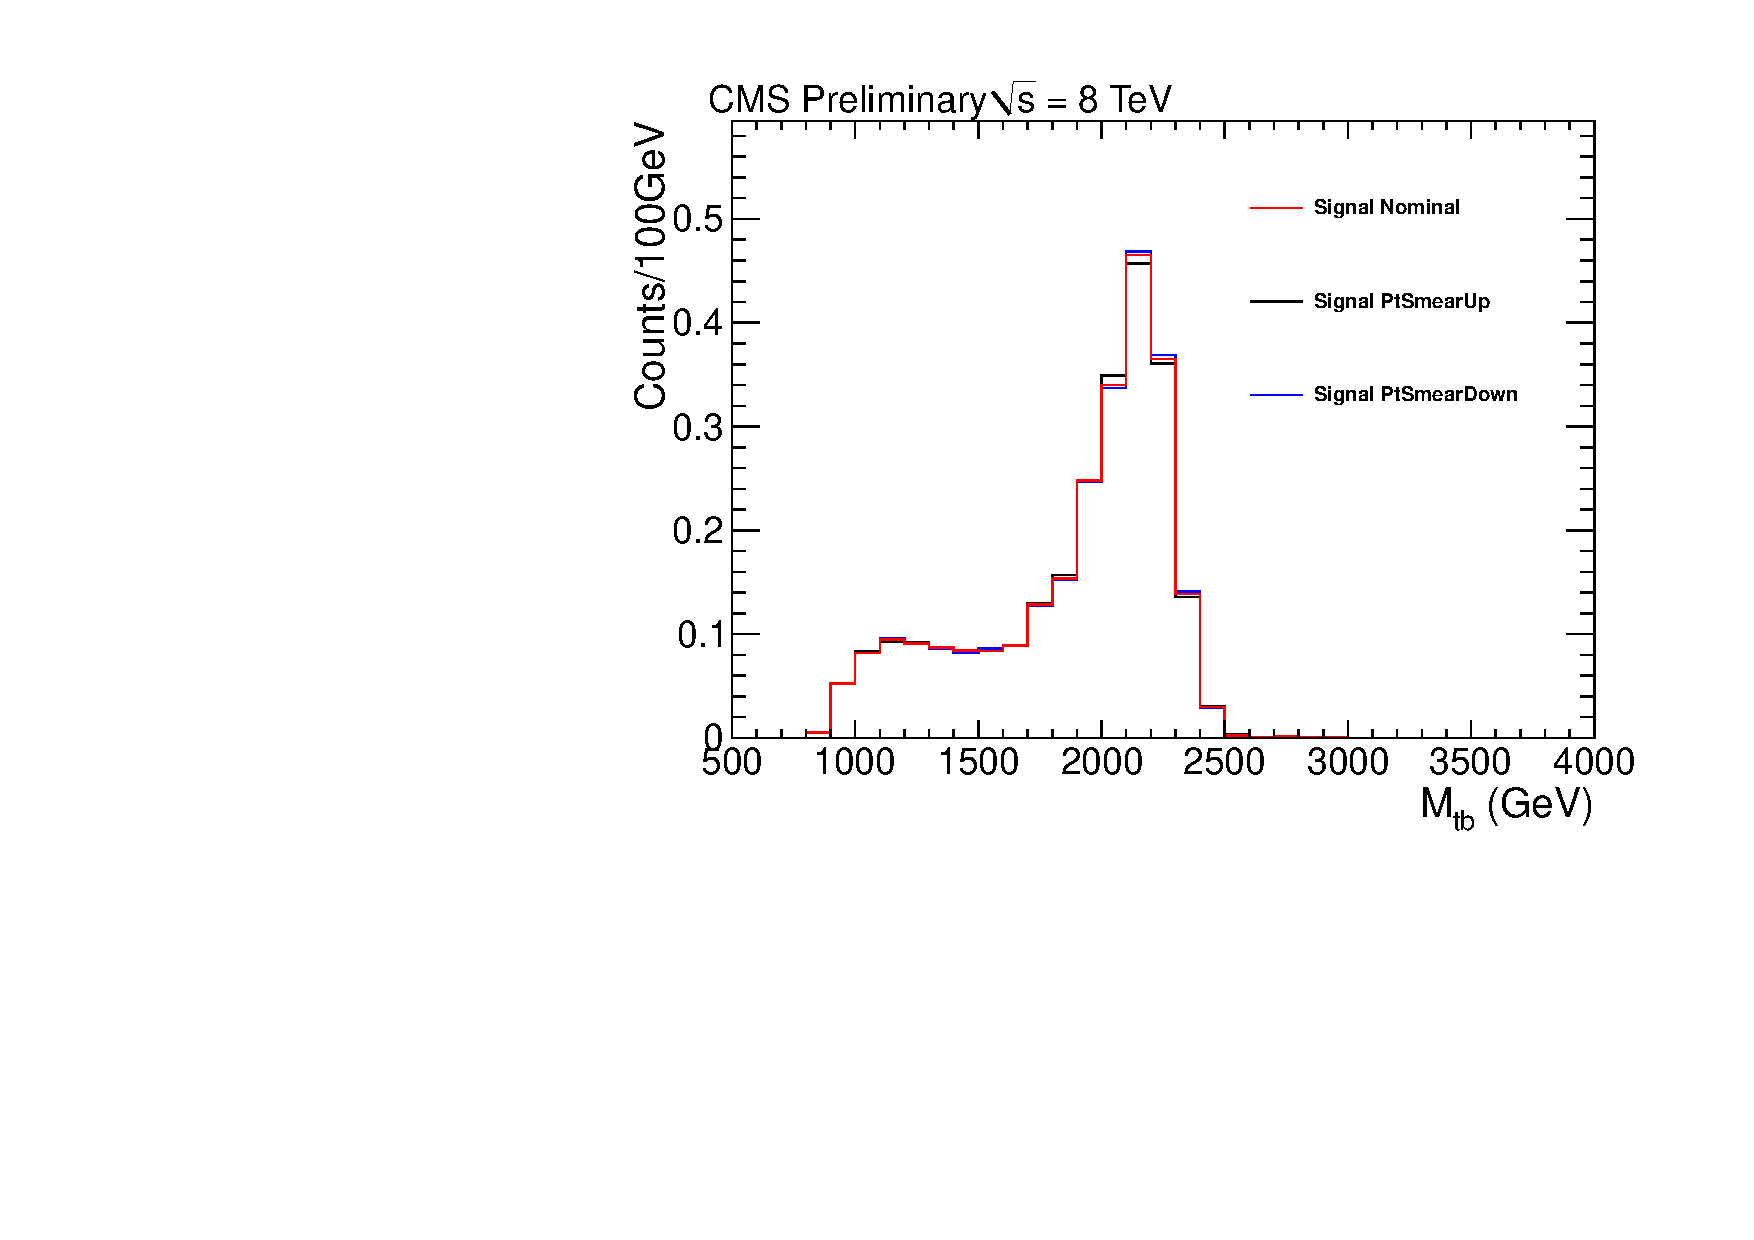
\includegraphics[width=0.45\textwidth]{AN-13-004/figs/Signal_M2300_PtSmearing}
\caption{
Jet Energy Resolution systematic variation for Right-handed $\wpr$ MC at the following mass points
(a) $M_{\wpr}$ = 1300$~\GeV$ 
(b) $M_{\wpr}$ = 1900$~\GeV$
(c) $M_{\wpr}$ = 2300$~\GeV$ 
}
\label{figs:signalJER}
\end{center}
\end{figure}

\begin{figure}[htcb]
\begin{center}
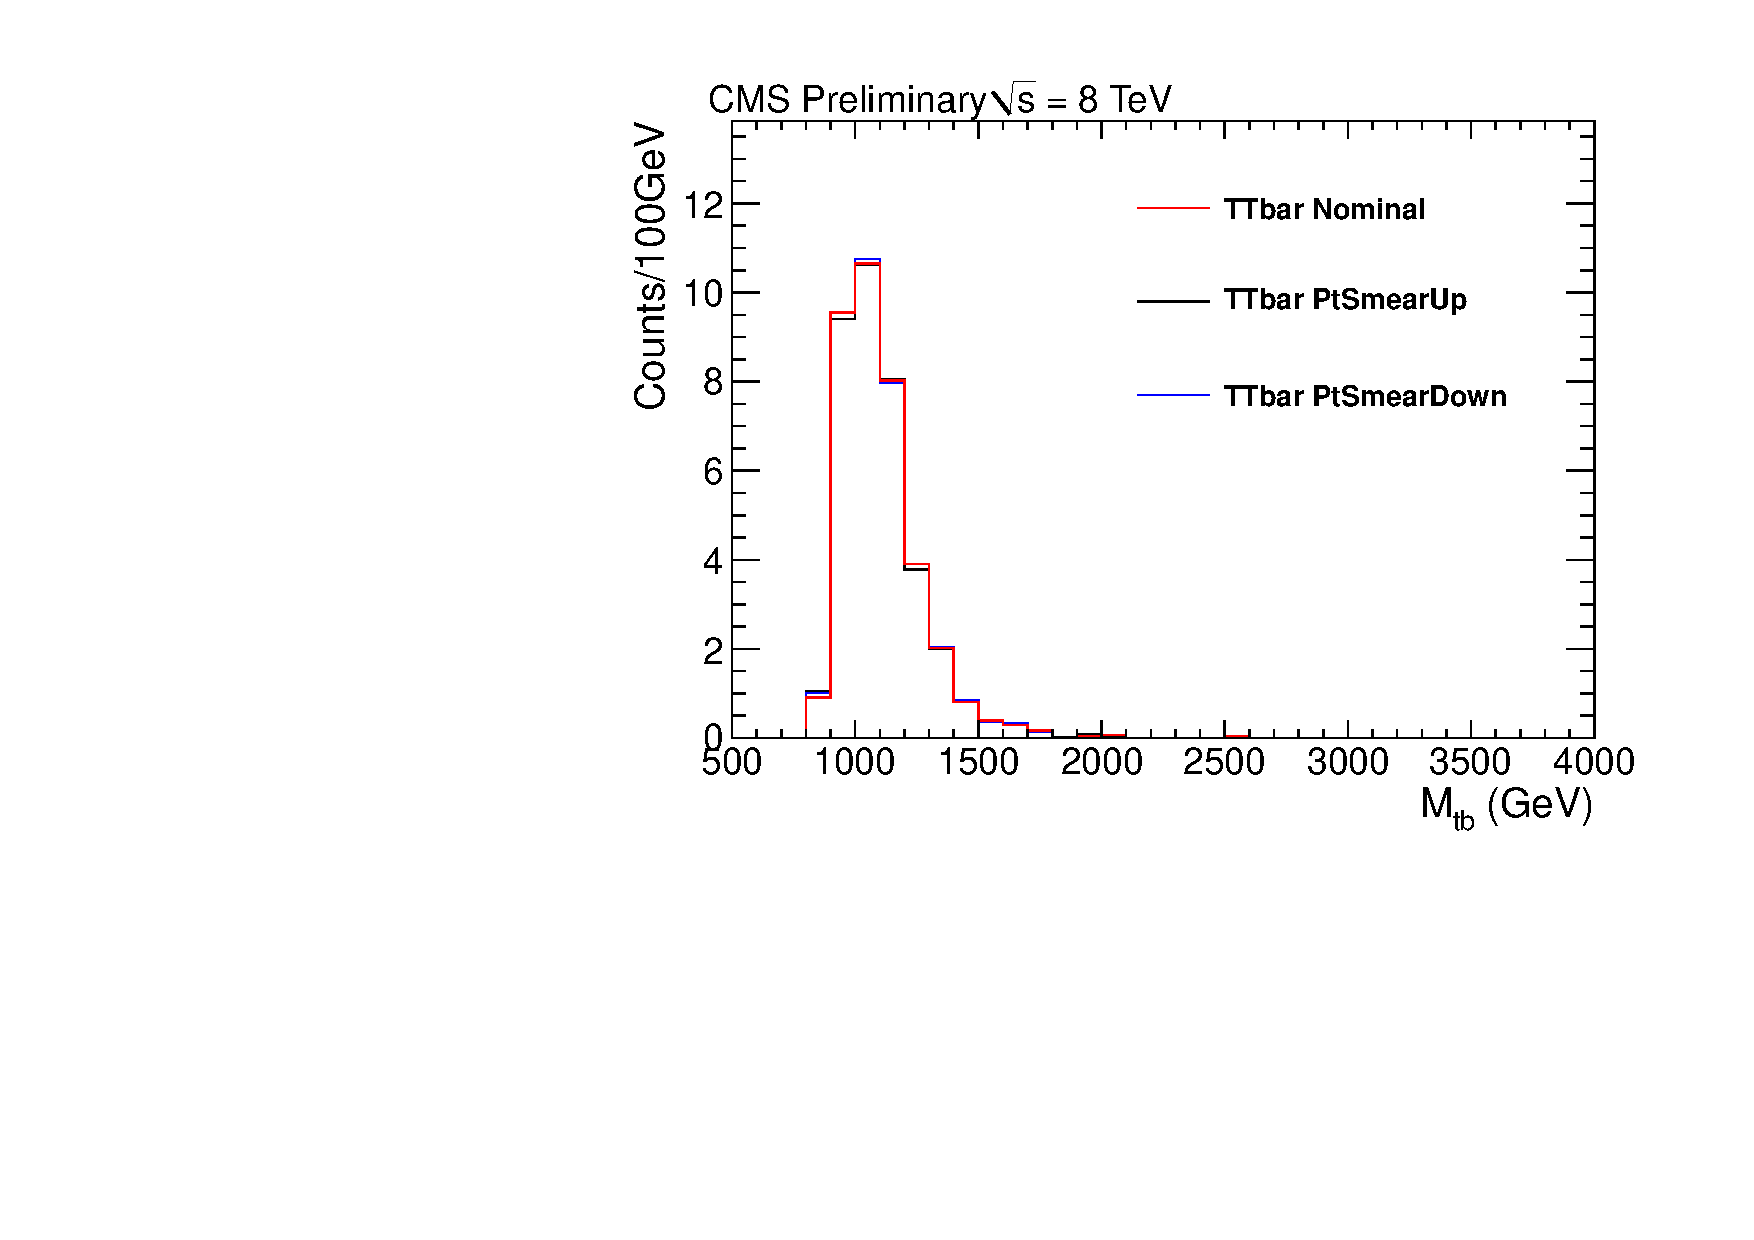
\includegraphics[width=0.7\textwidth]{AN-13-004/figs/TTbar_PtSmearing}
\caption{Jet Energy Resolution systematic variation for $\ttbar$ MC}
\label{figs:ttbarJER}
\end{center}
\end{figure}

\begin{figure}[htcb]
\begin{center}
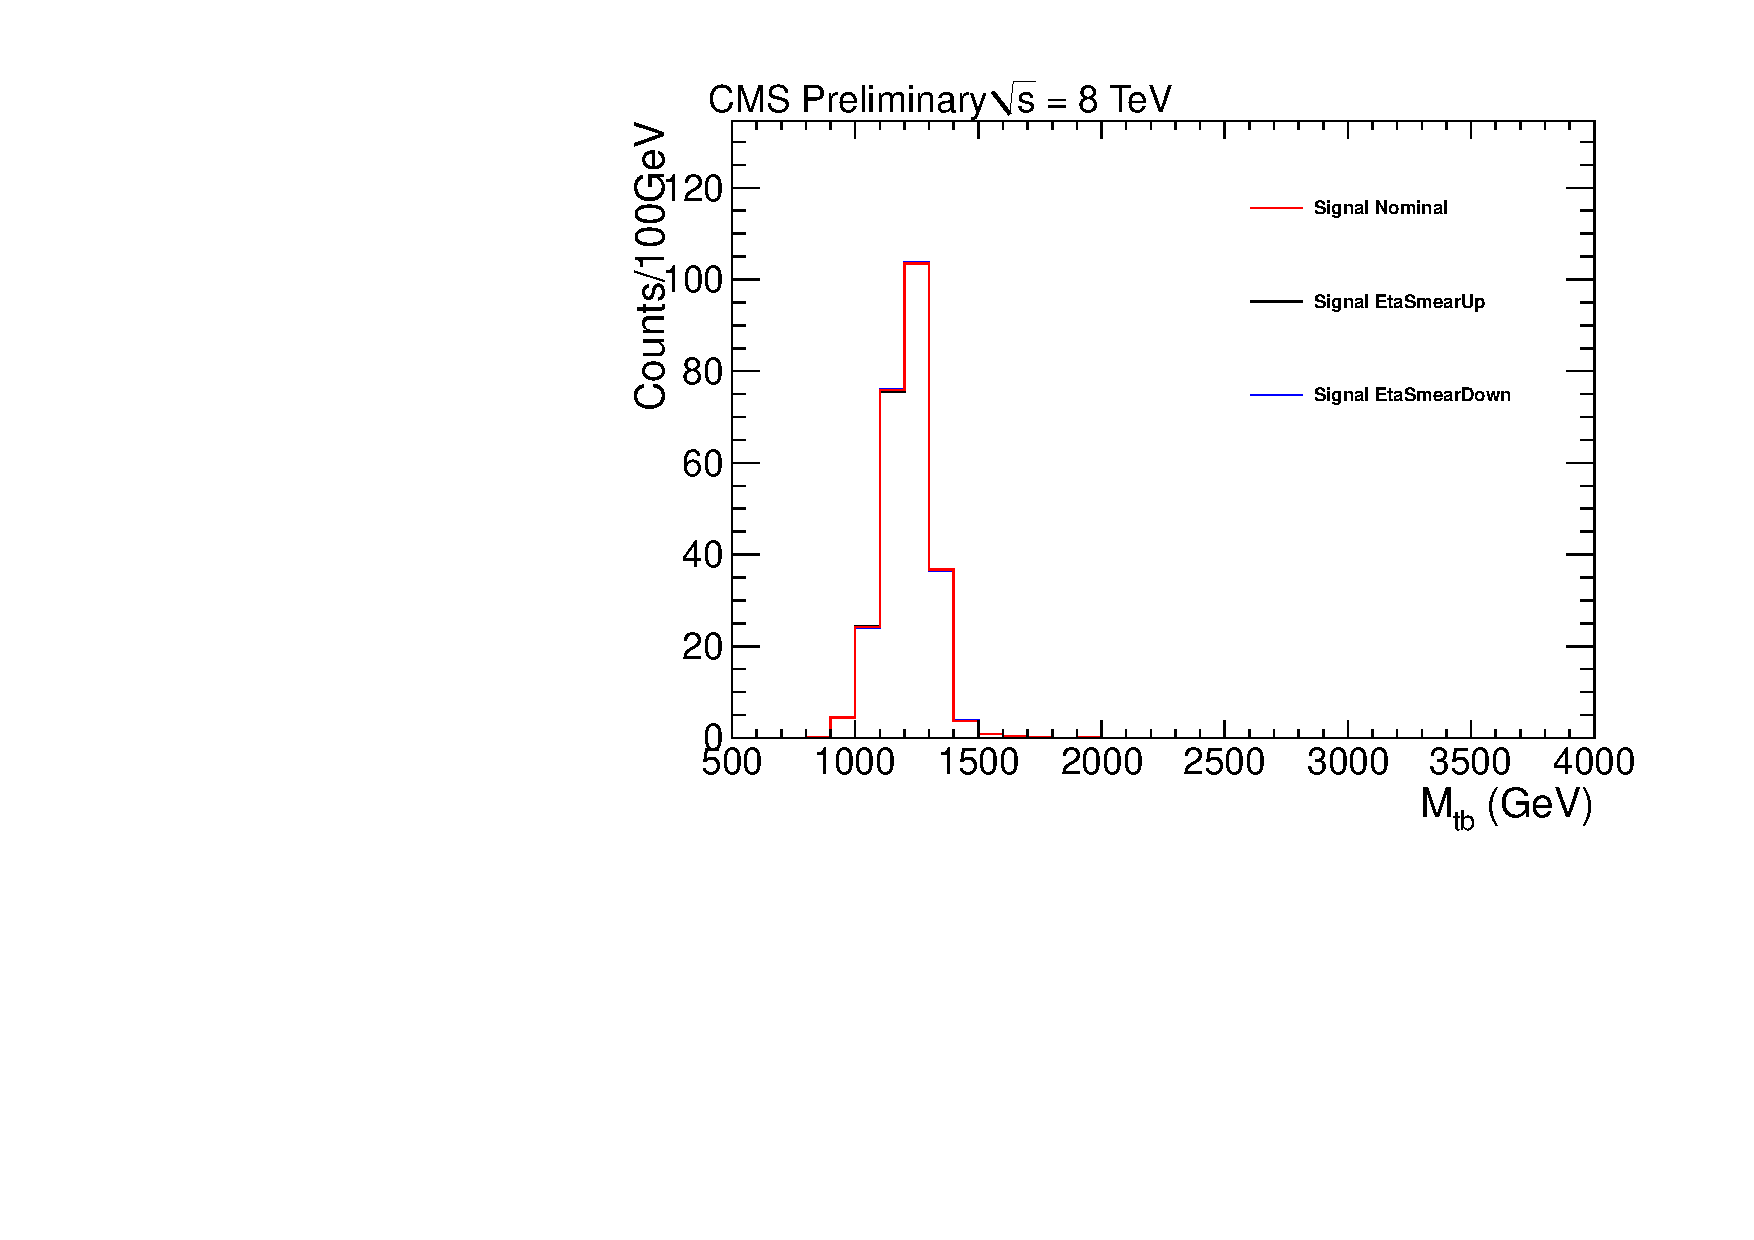
\includegraphics[width=0.45\textwidth]{AN-13-004/figs/Signal_M1300_EtaScaling}
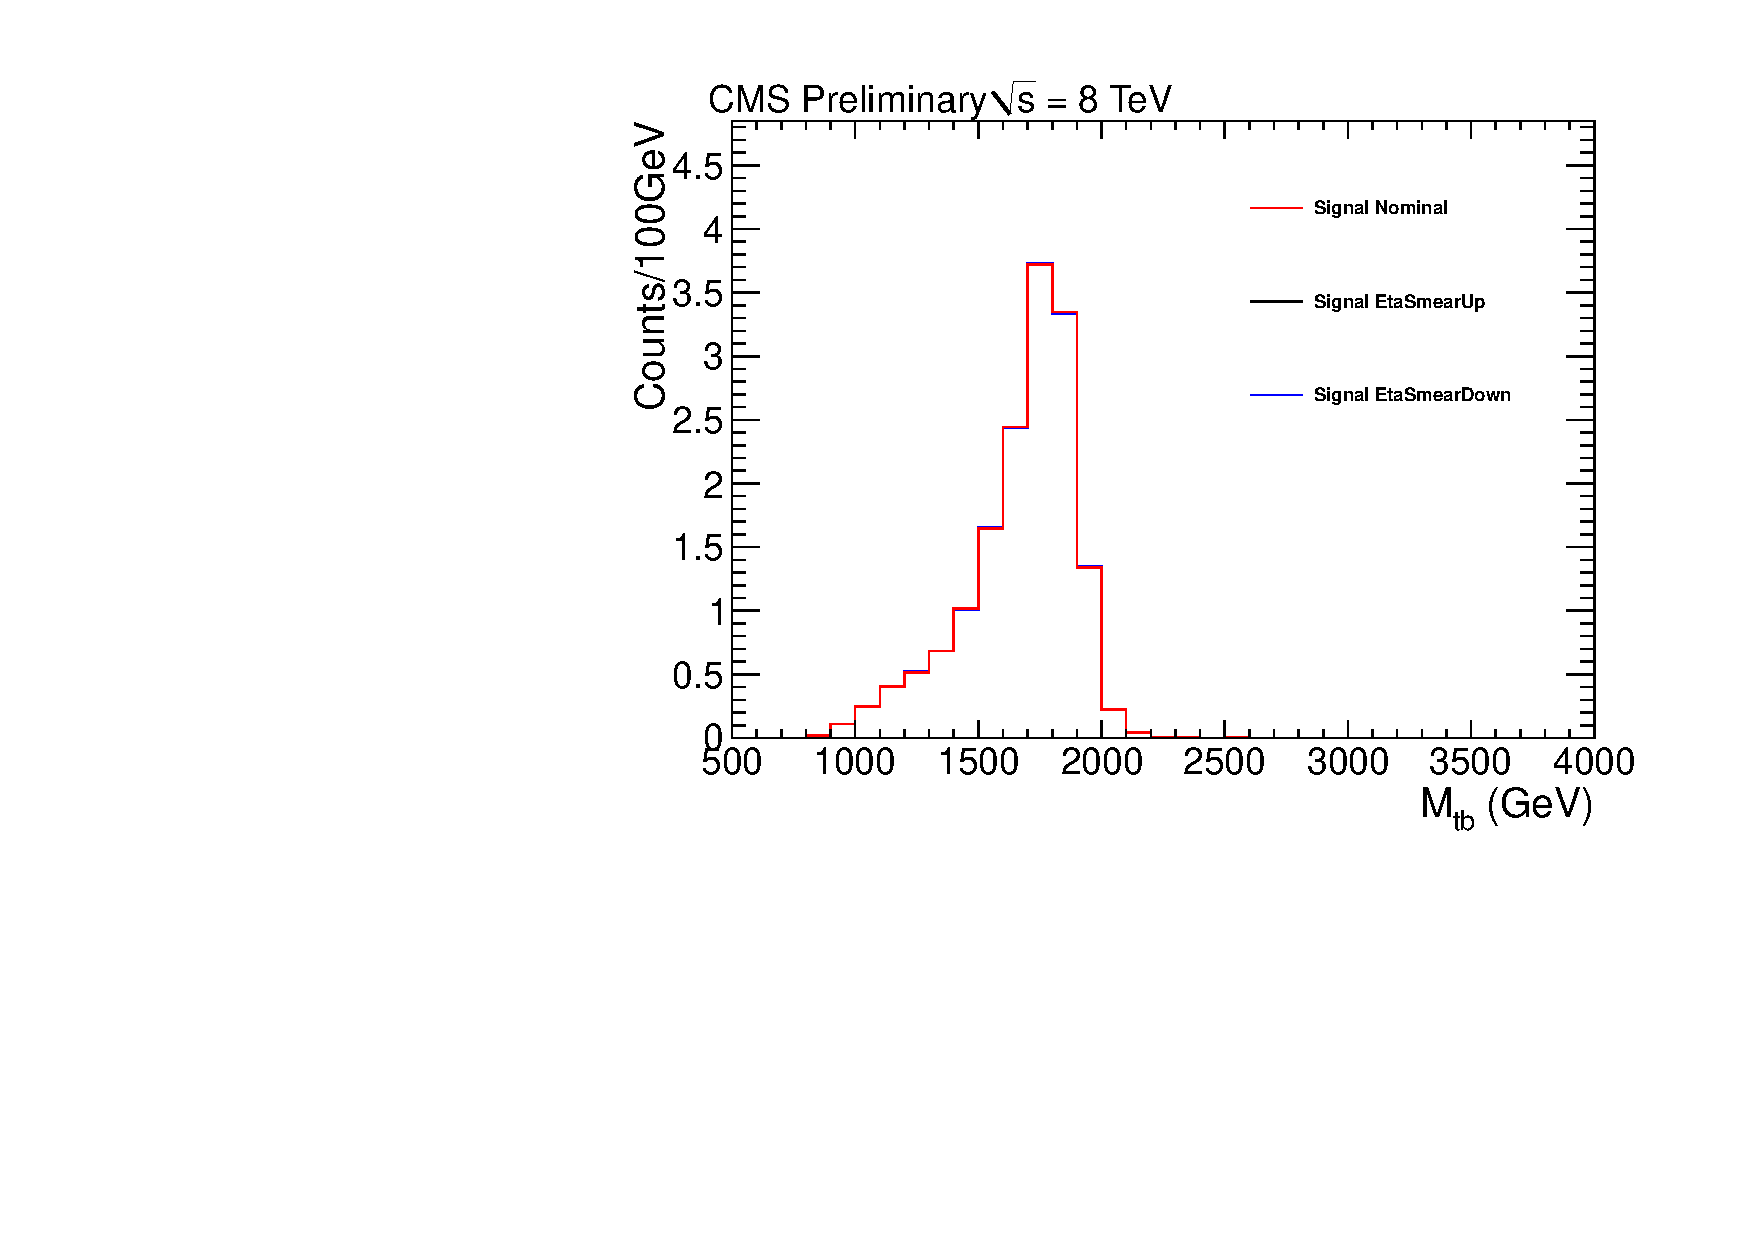
\includegraphics[width=0.45\textwidth]{AN-13-004/figs/Signal_M1900_EtaScaling}
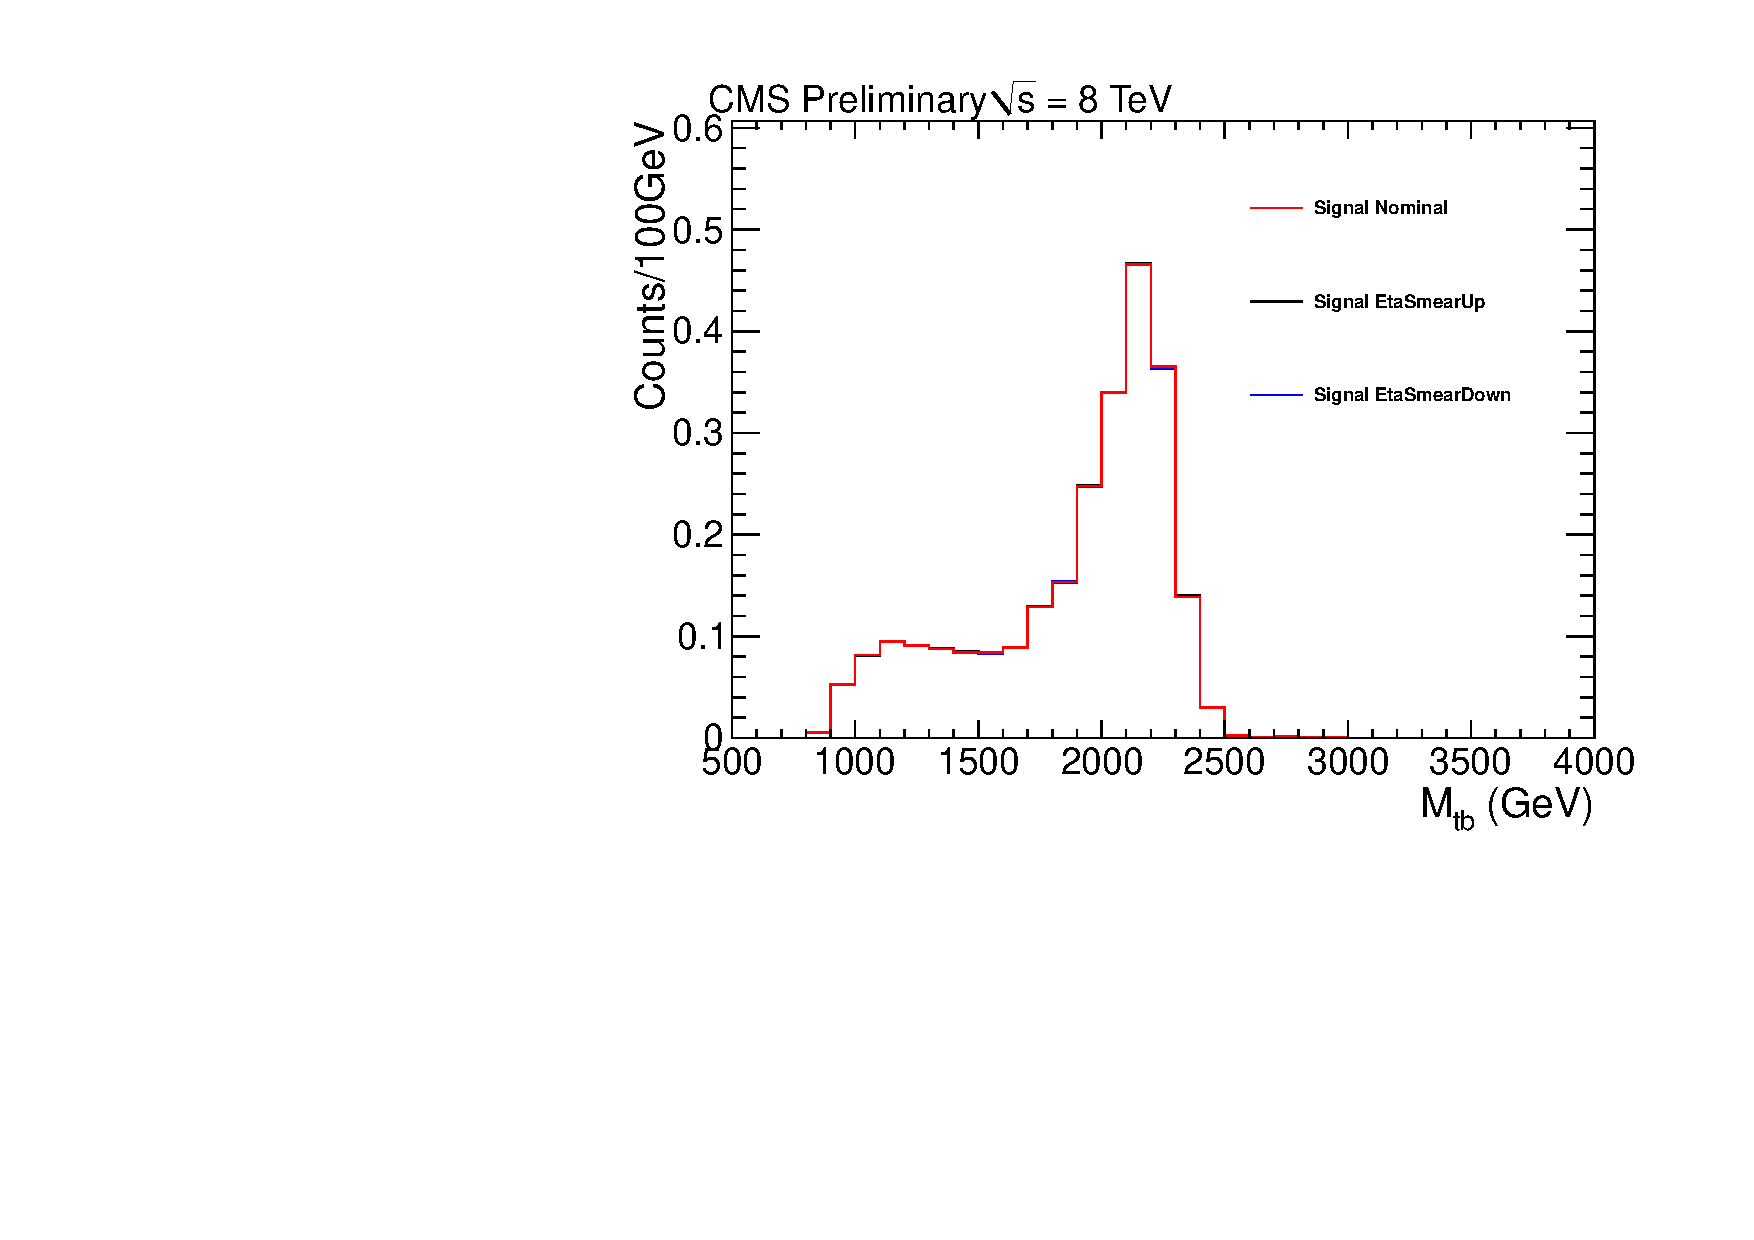
\includegraphics[width=0.45\textwidth]{AN-13-004/figs/Signal_M2300_EtaScaling}
\caption{
Jet Angular Resolution systematic variation for Right-handed $\wpr$ MC at the following mass points
(a) $M_\wpr$ = 1300$~\GeV$ 
(b) $M_\wpr$ = 1900$~\GeV$
(c) $M_\wpr$ = 2300$~\GeV$ 
}
\label{figs:signalJAR}
\end{center}
\end{figure}

\begin{figure}[htcb]
\begin{center}
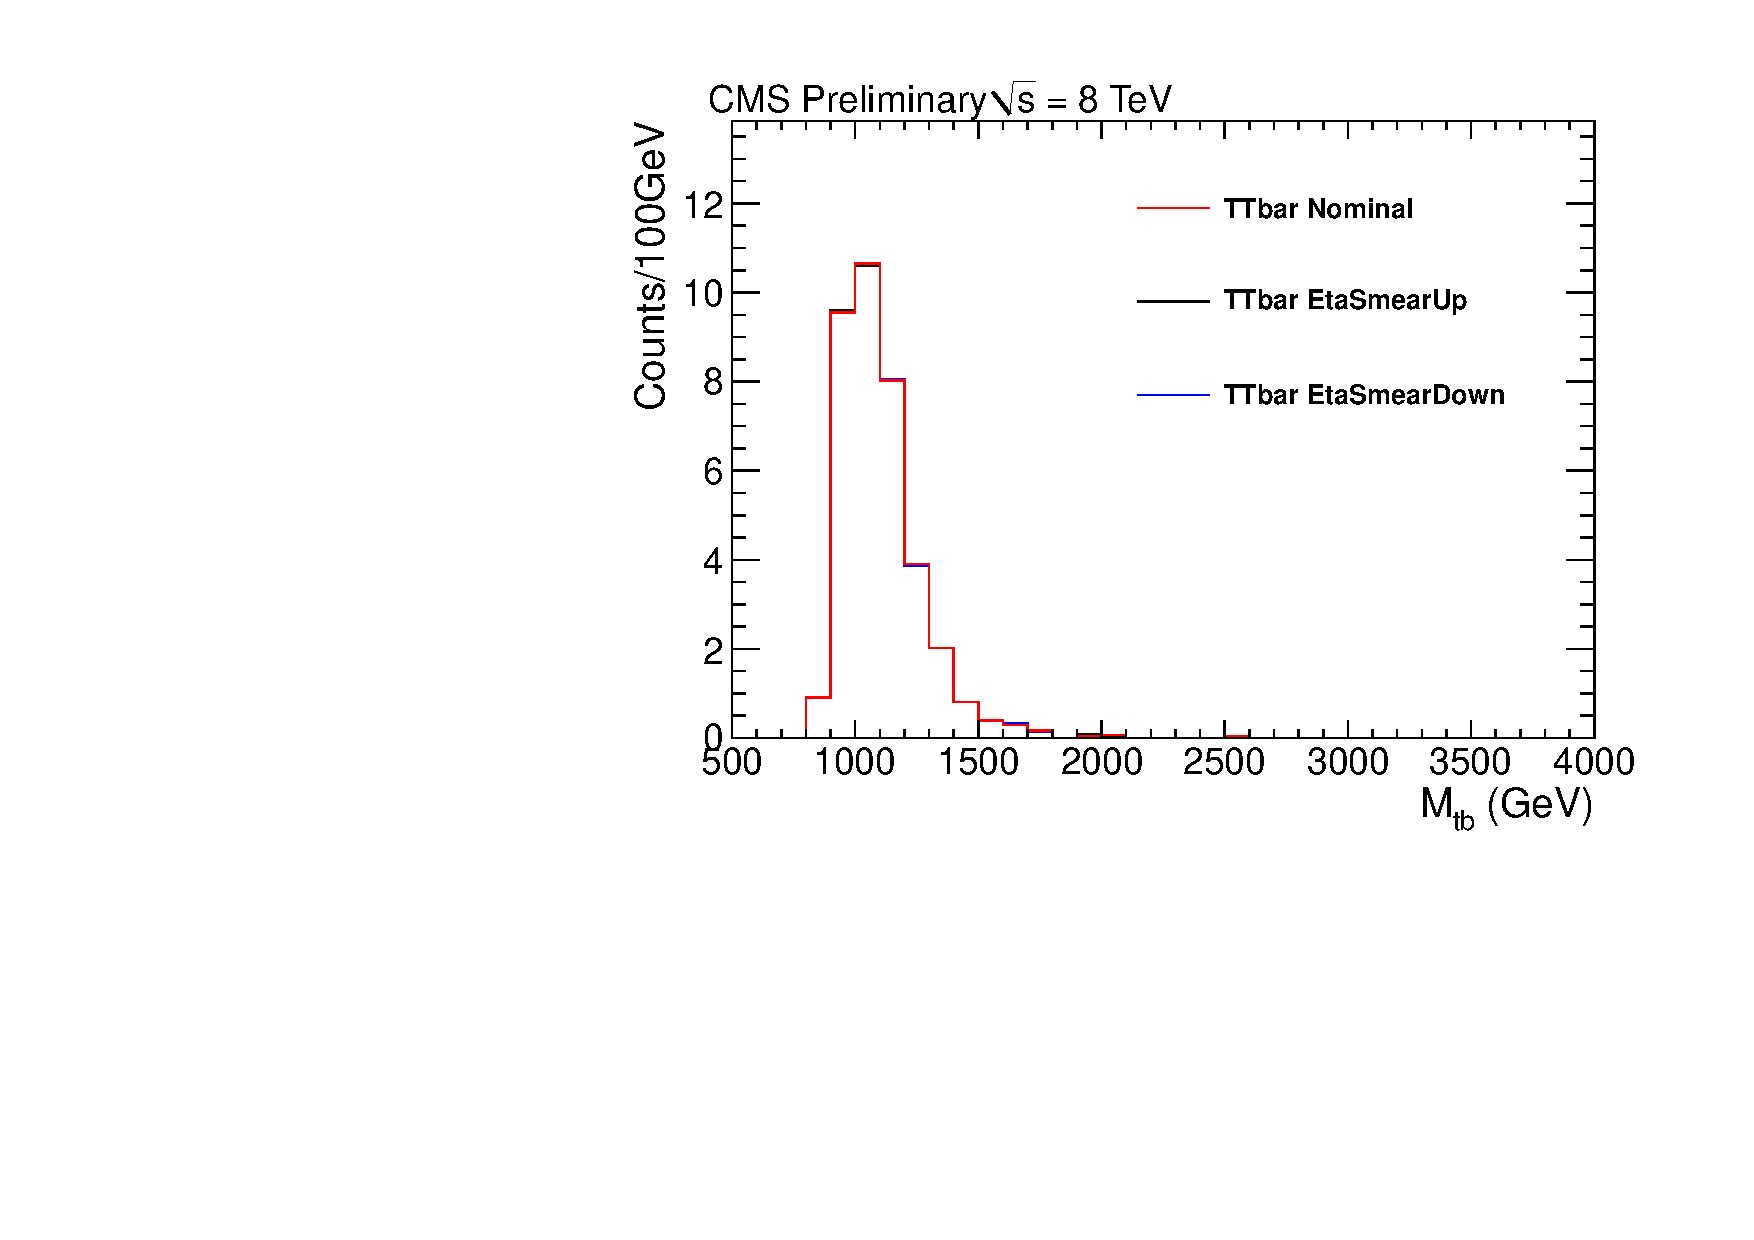
\includegraphics[width=0.7\textwidth]{AN-13-004/figs/TTbar_EtaScaling}
\caption{Jet Angular Resolution systematic variation for $\ttbar$ MC}
\label{figs:ttbarJAR}
\end{center}
\end{figure}

\begin{figure}[htcb]
\begin{center}
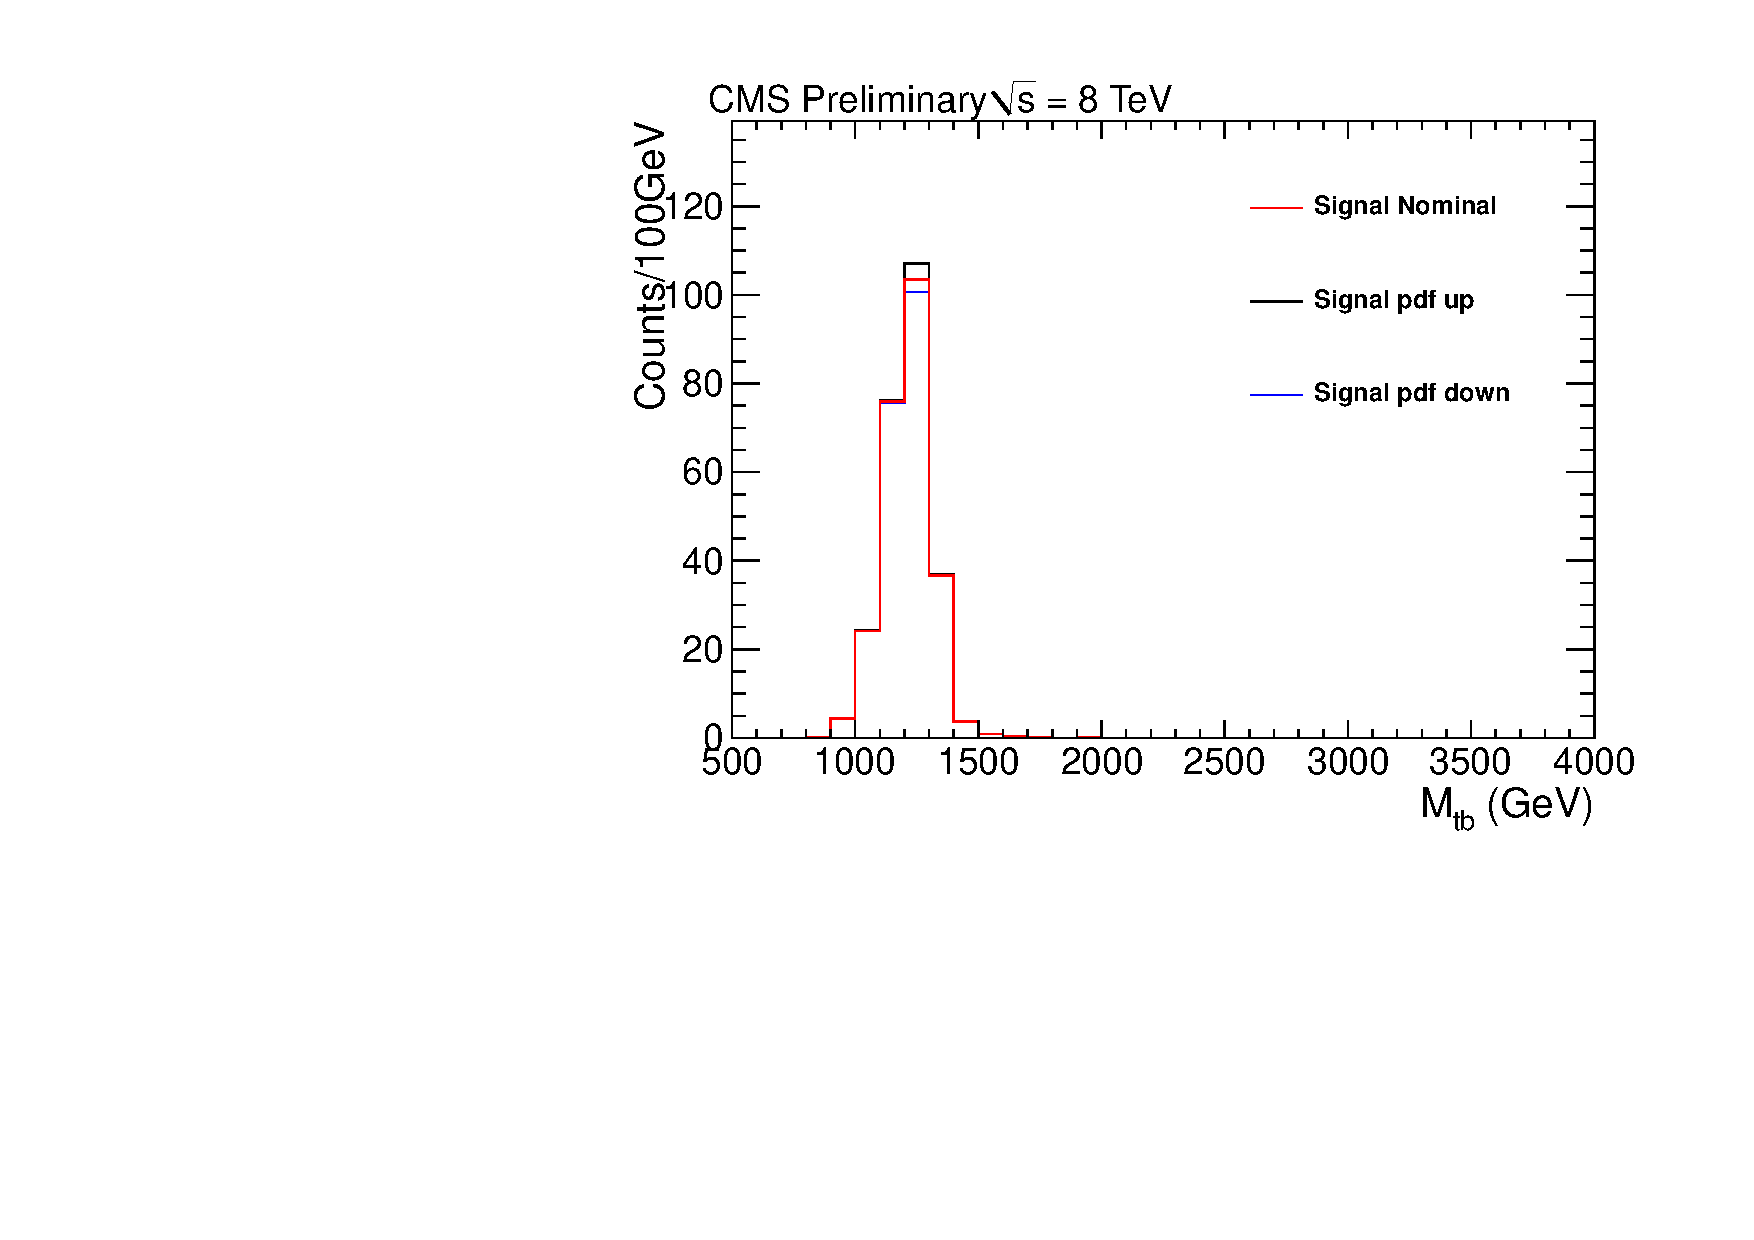
\includegraphics[width=0.45\textwidth]{AN-13-004/figs/Signal_M1300_PdfScaleNNPDF23.pdf}
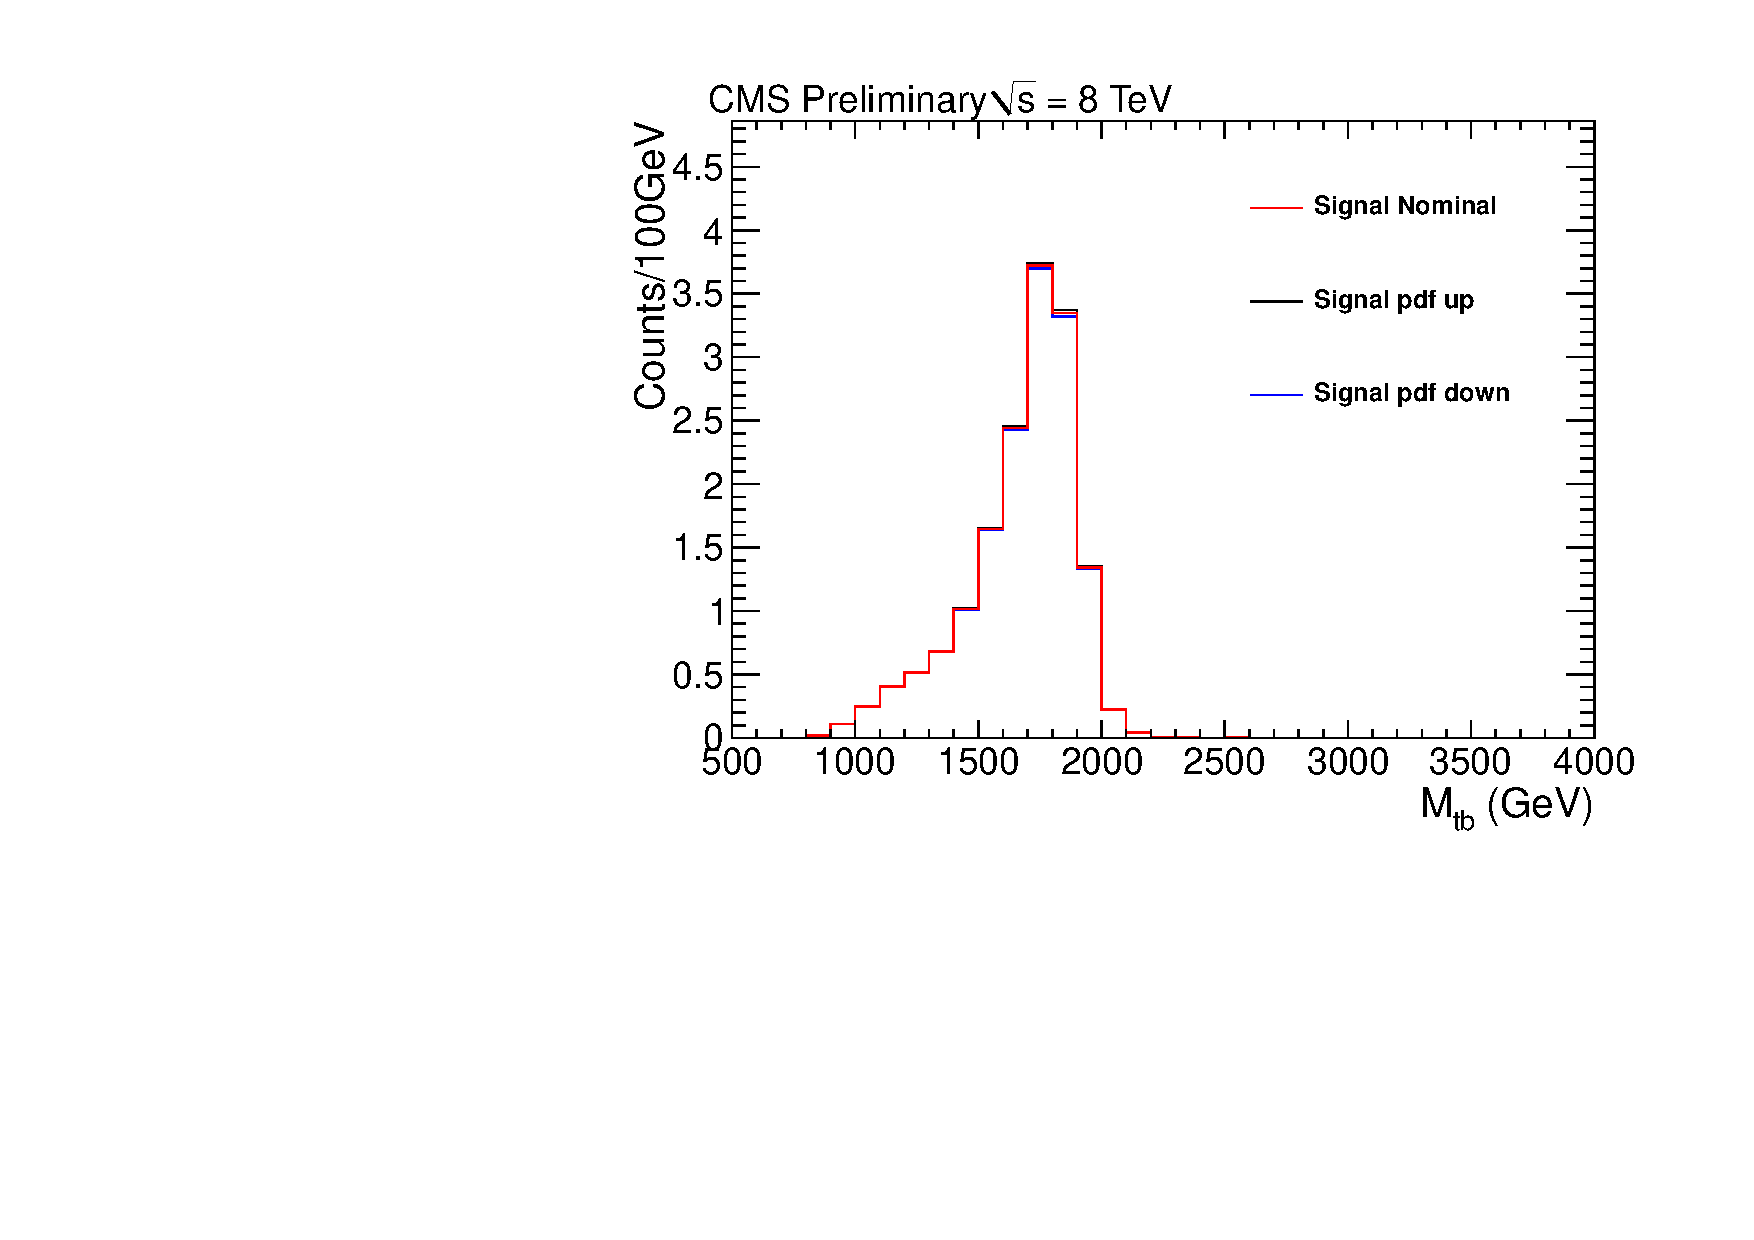
\includegraphics[width=0.45\textwidth]{AN-13-004/figs/Signal_M1900_PdfScaleNNPDF23.pdf}
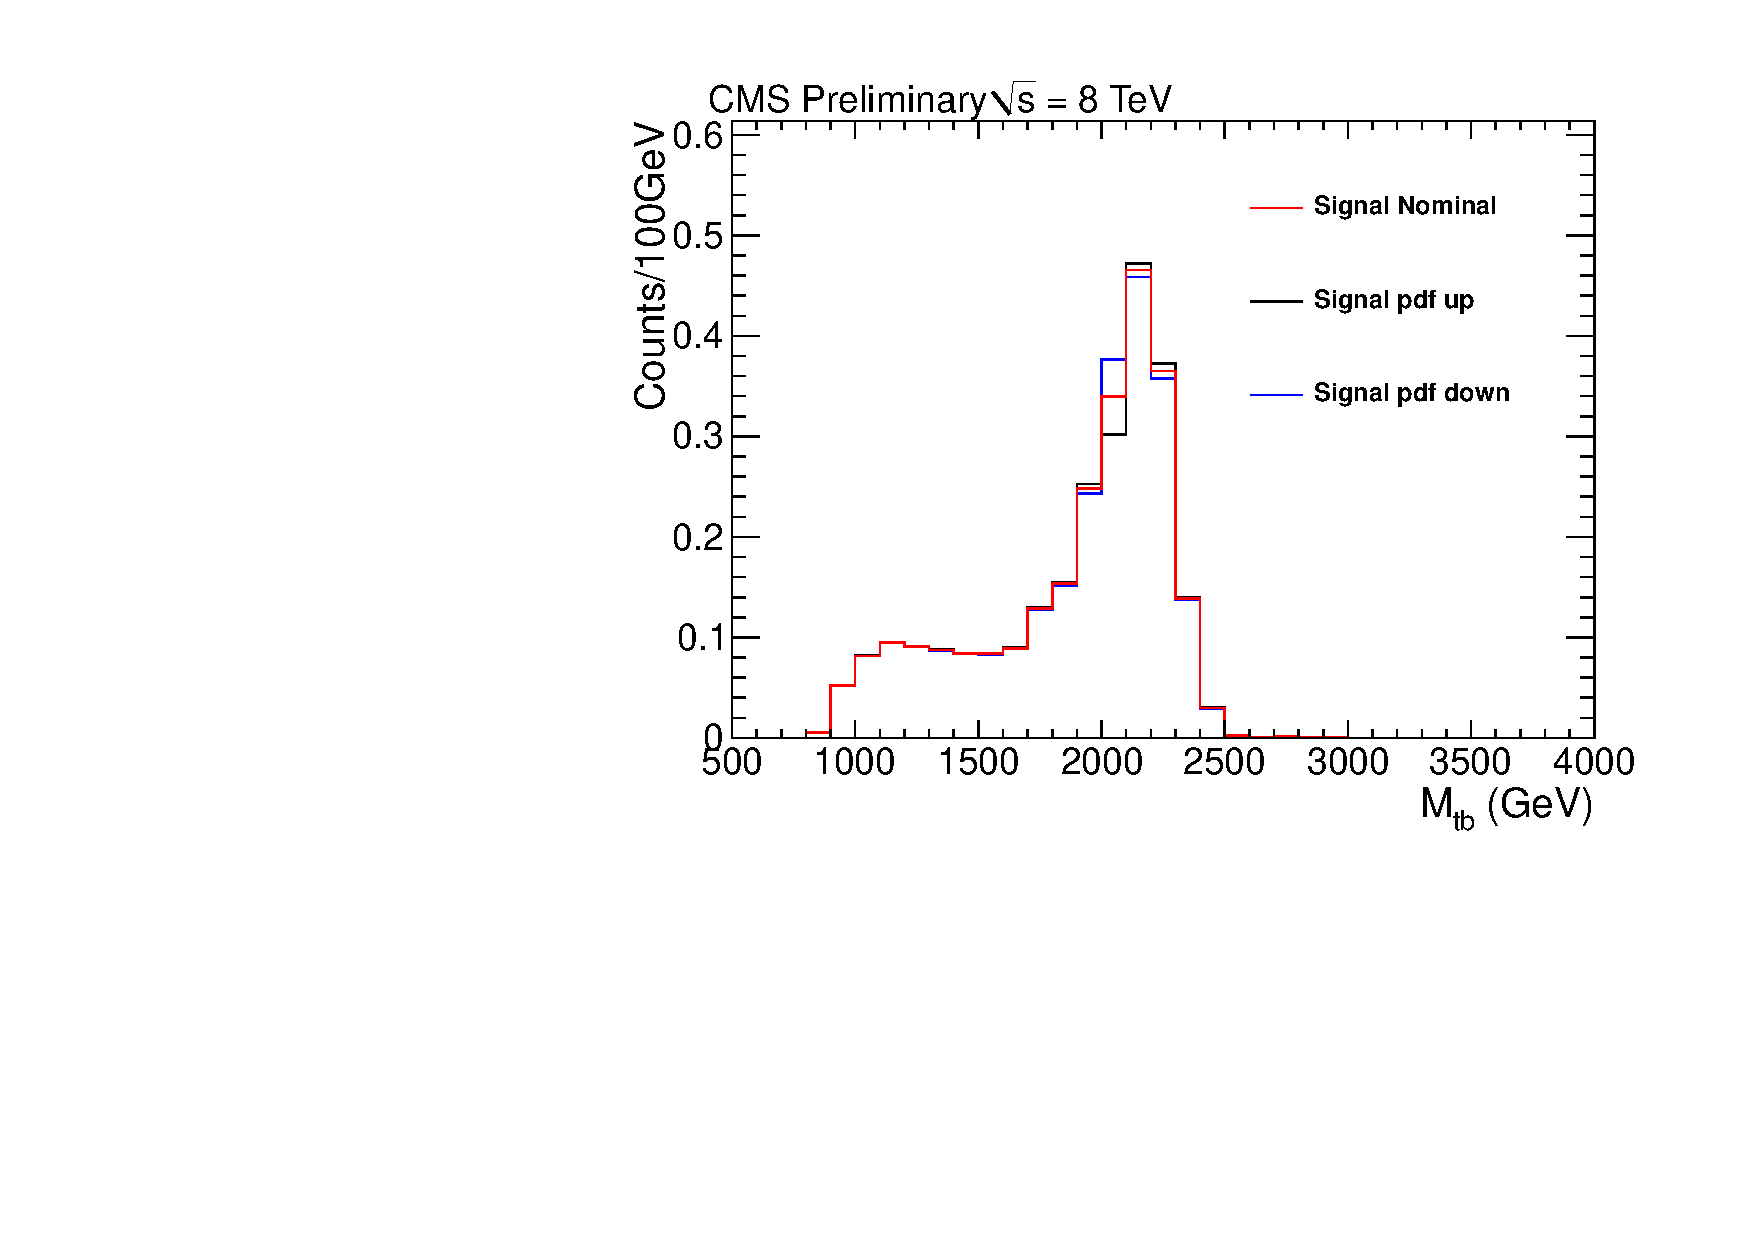
\includegraphics[width=0.45\textwidth]{AN-13-004/figs/Signal_M2300_PdfScaleNNPDF23.pdf}
\caption{
PDF systematic variation for Right-handed $\wpr$ MC at the following mass points
(a) $M_\wpr$ = 1300$~\GeV$ 
(b) $M_\wpr$ = 1900$~\GeV$
(c) $M_\wpr$ = 2300$~\GeV$ 
}
\label{figs:signalPDF}
\end{center}
\end{figure}

\begin{figure}[htcb]
\begin{center}
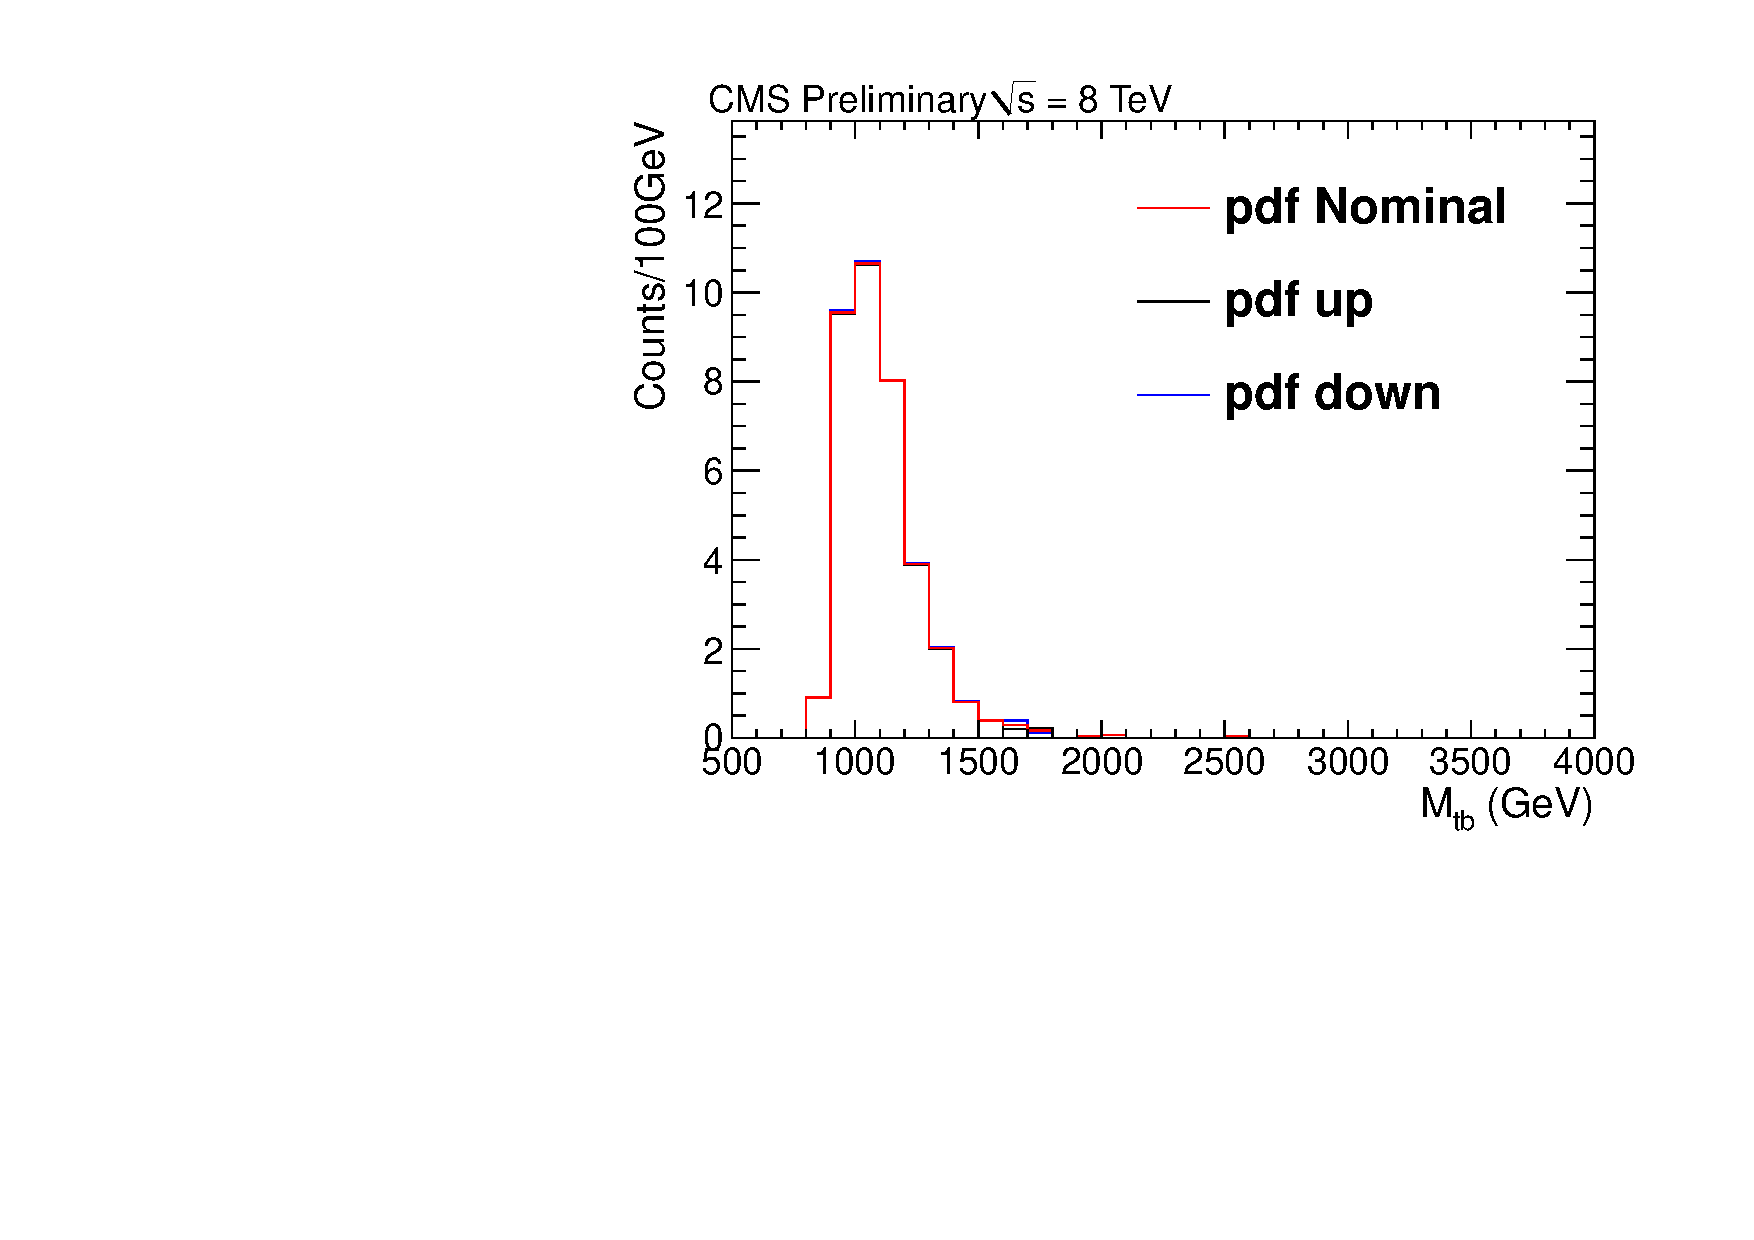
\includegraphics[width=0.7\textwidth]{AN-13-004/figs/TTbar_PdfScaleNNPDF23.pdf}
\caption{PDF systematic variation for $\ttbar$ MC}
\label{figs:ttbarPDF}
\end{center}
\end{figure}

\begin{figure}[htcb]
\begin{center}
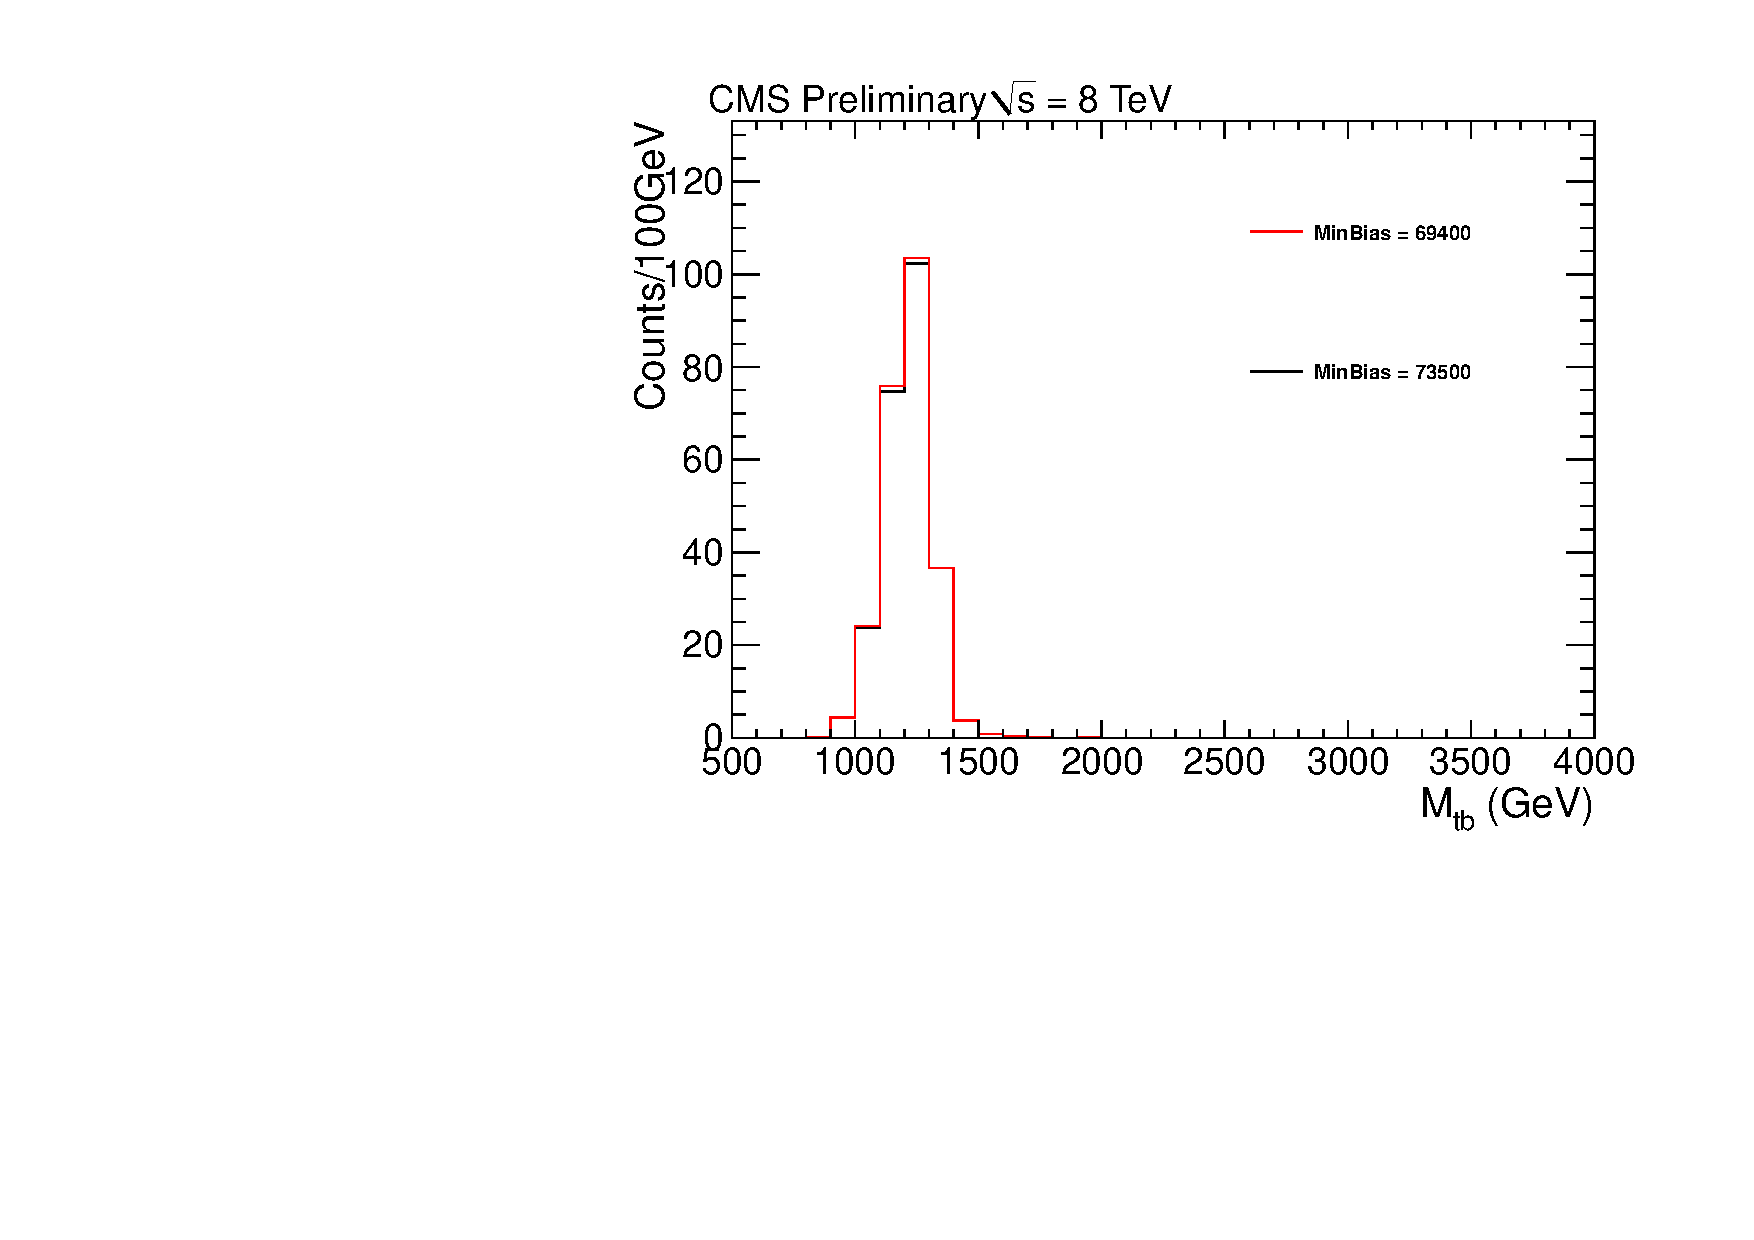
\includegraphics[width=0.45\textwidth]{AN-13-004/figs/Signal_M1300_PileupReweighting}
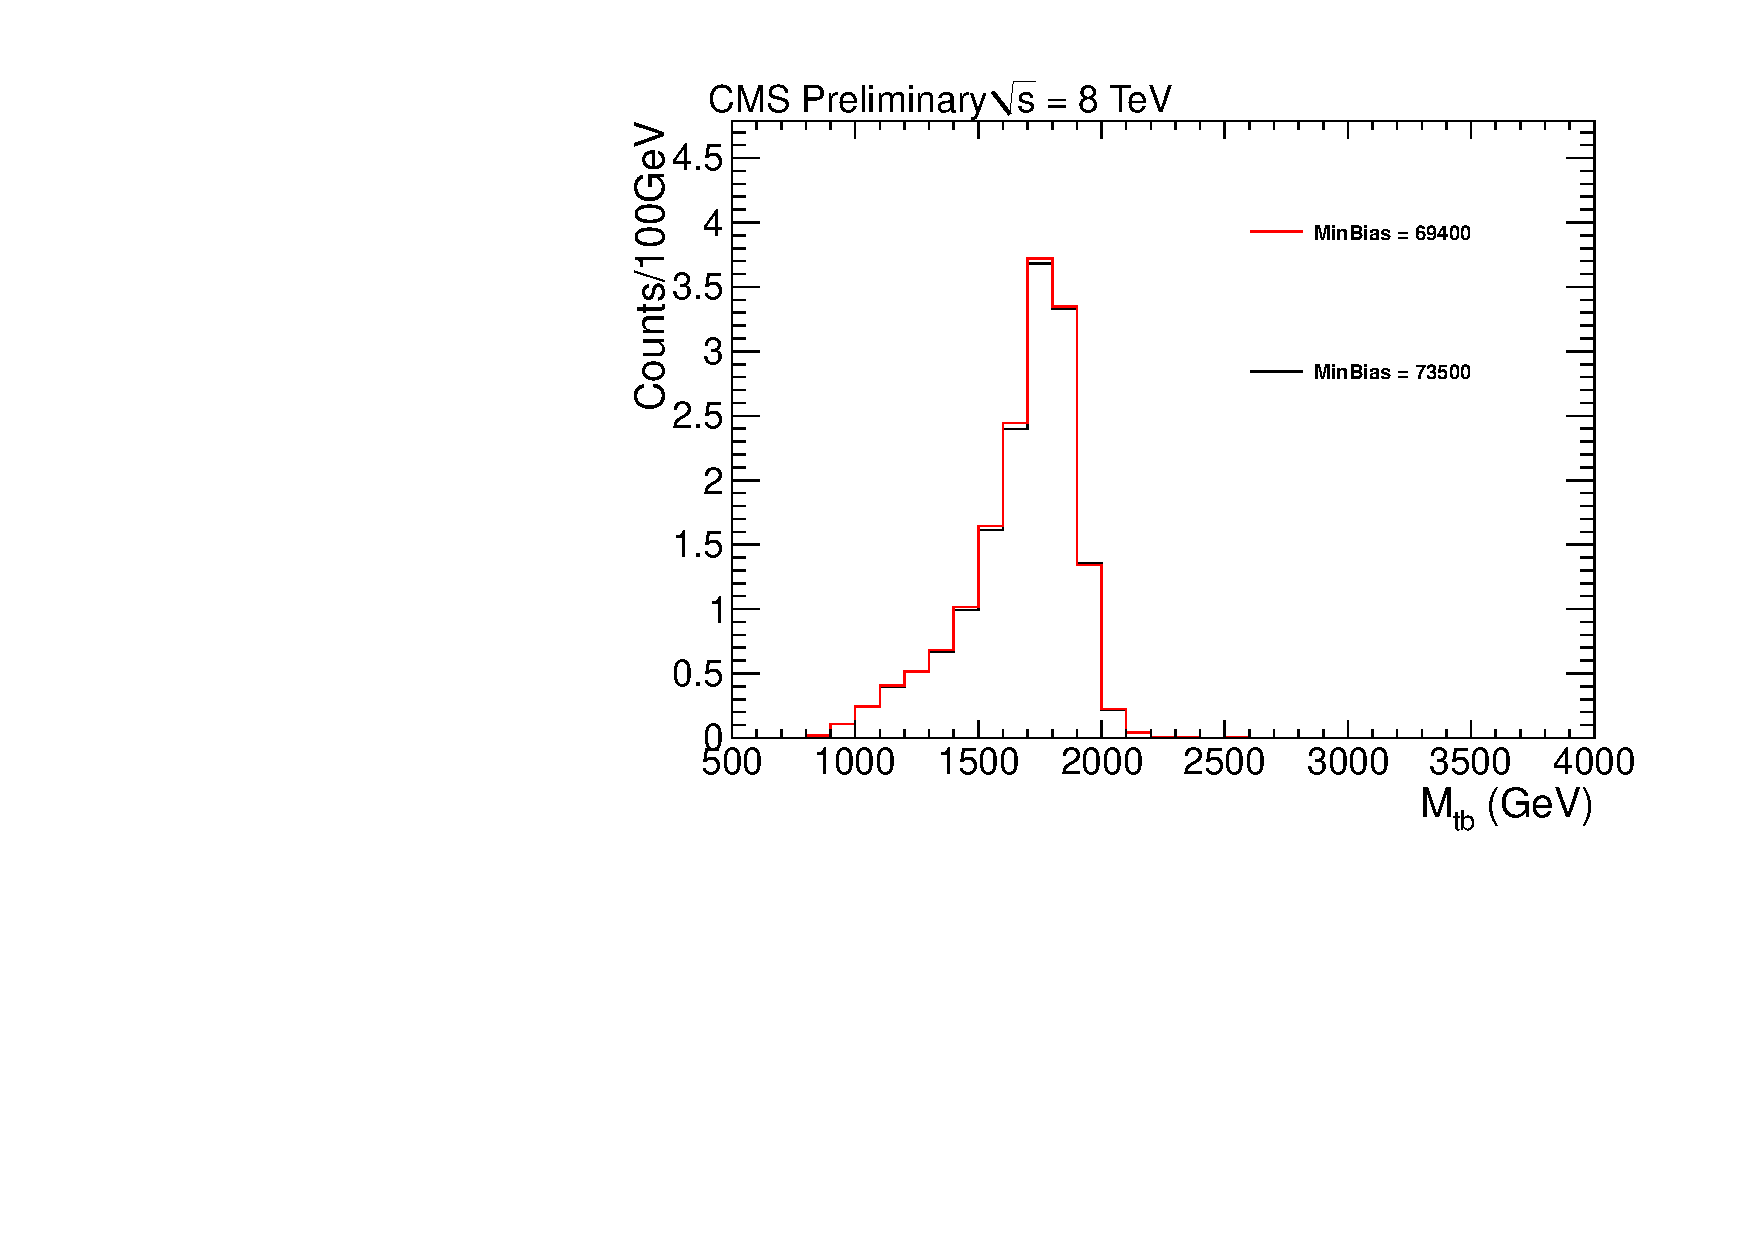
\includegraphics[width=0.45\textwidth]{AN-13-004/figs/Signal_M1900_PileupReweighting}
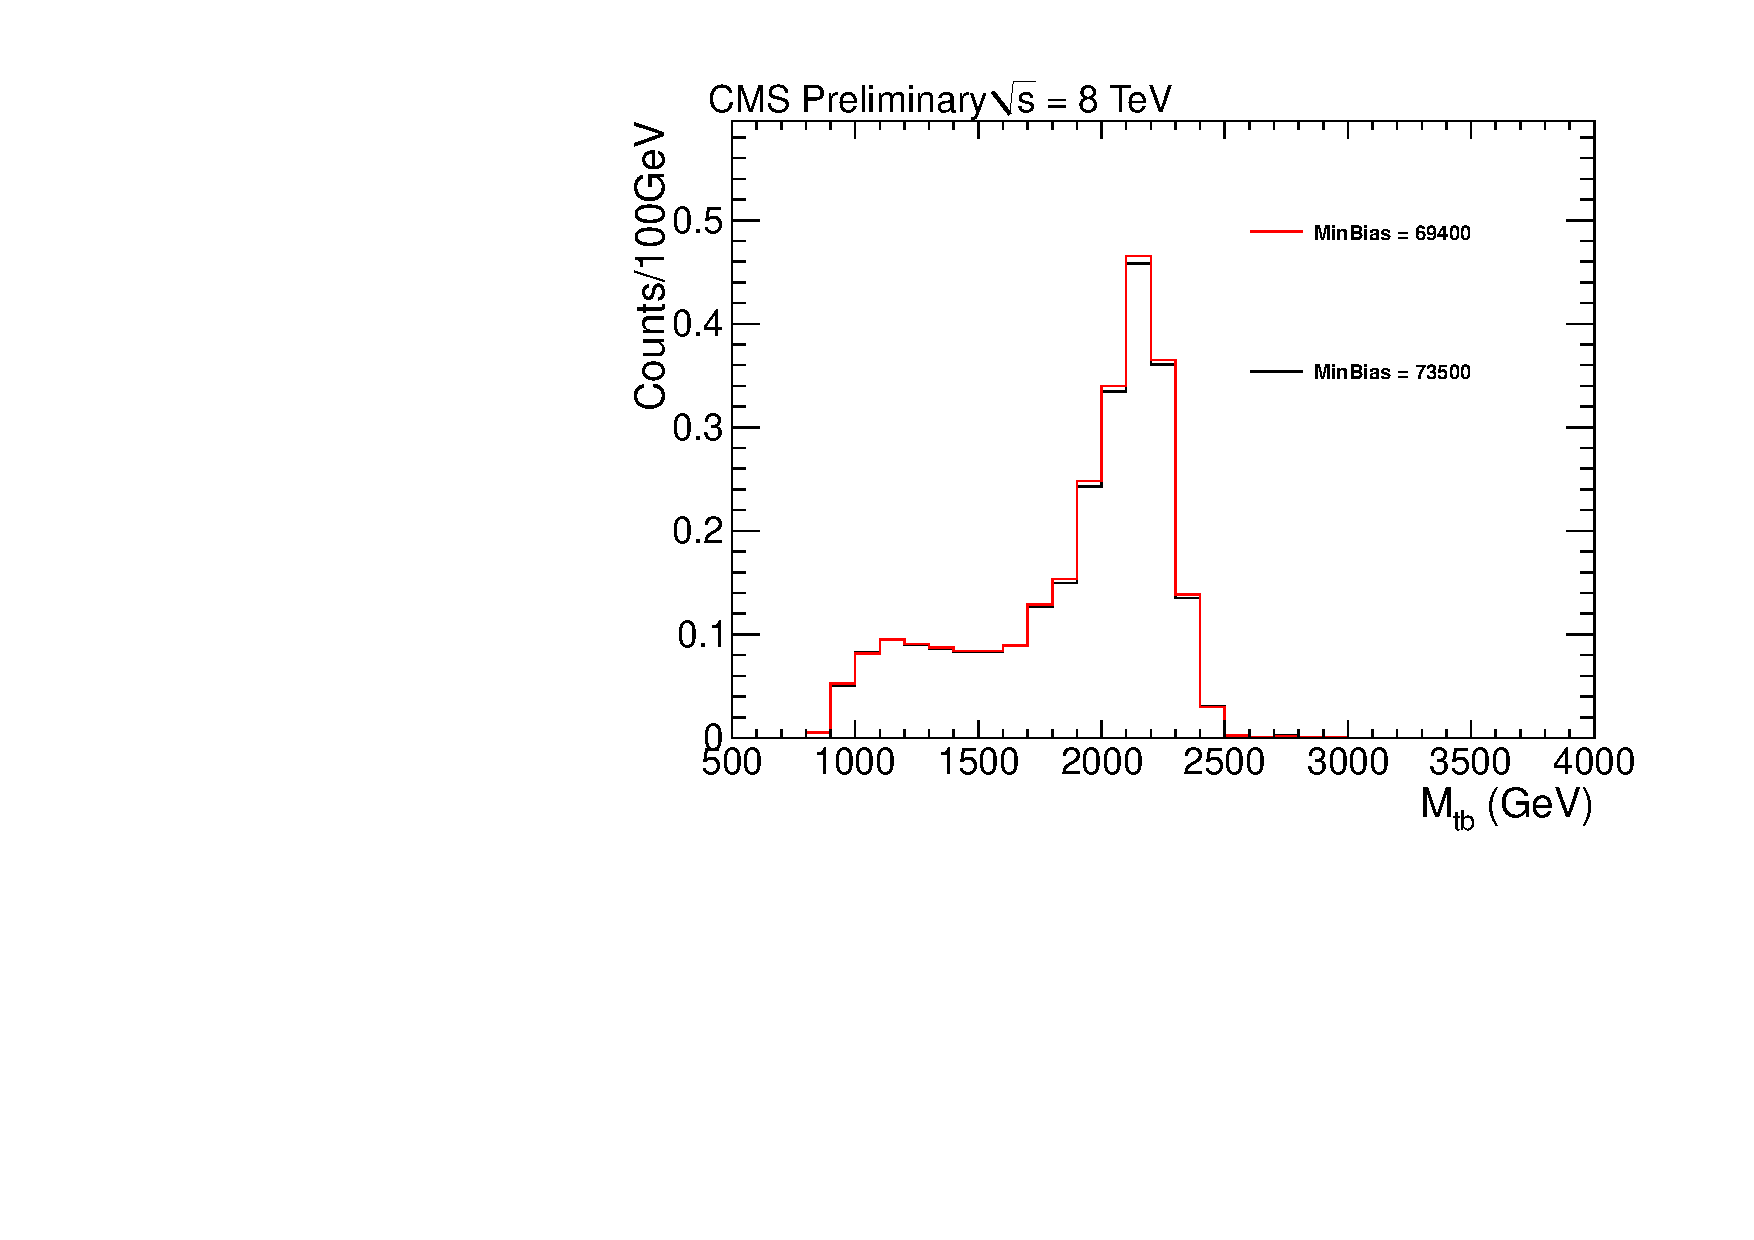
\includegraphics[width=0.45\textwidth]{AN-13-004/figs/Signal_M2300_PileupReweighting}
\caption{
Pileup systematic variation for Right-handed $\wpr$ MC at the following mass points
(a) $M_{\wpr}$ = 1300$~\GeV$ 
(b) $M_{\wpr}$ = 1900$~\GeV$
(c) $M_{\wpr}$ = 2300$~\GeV$ 
}
\label{figs:signalPU}
\end{center}
\end{figure}

%\begin{figure}[htcb]
%\begin{center}
%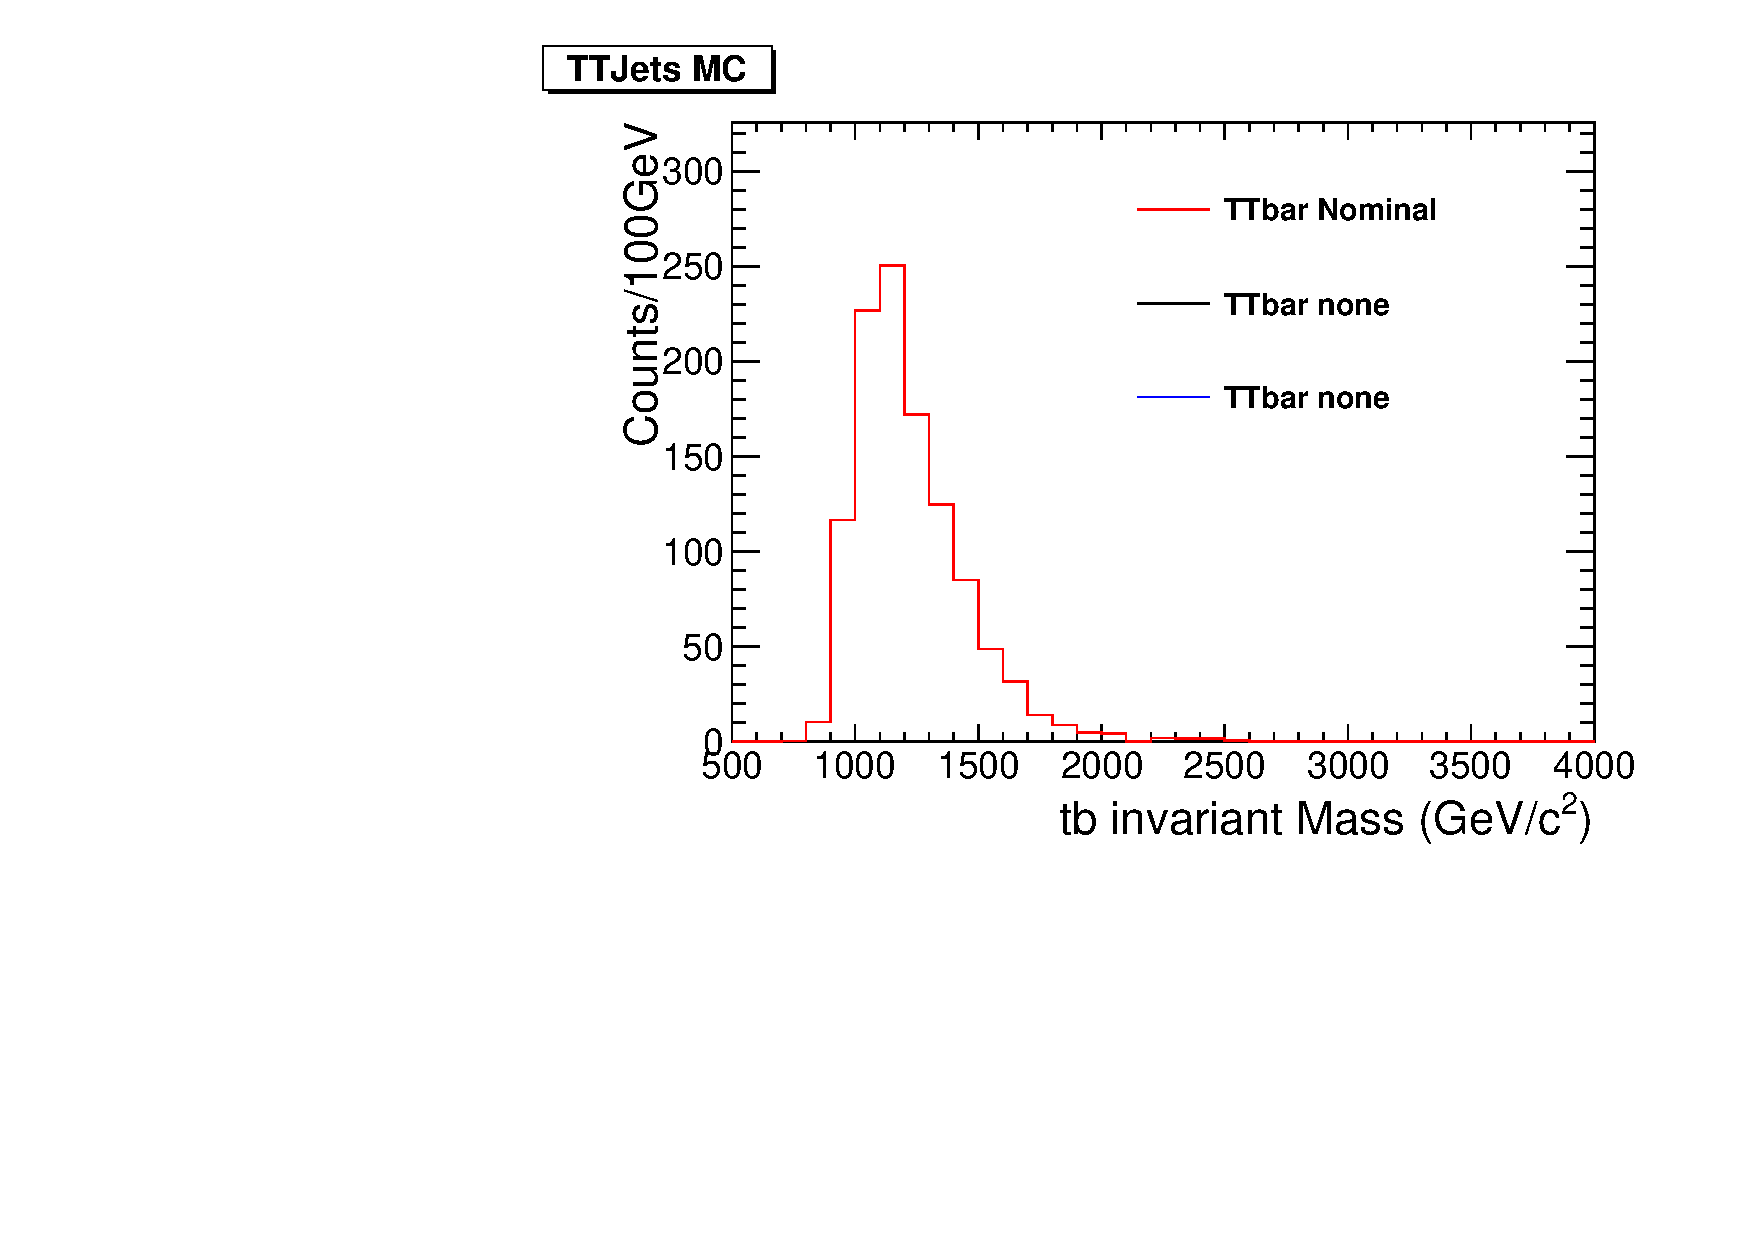
\includegraphics[width=0.7\textwidth]{AN-13-004/figs/TTbar_PileupReweighting}
%\caption{Pileup systematic variation for $\ttbar$ MC}
%\label{figs:ttbarPU}
%\end{center}
%\end{figure}

\begin{figure}[htcb]
\begin{center}
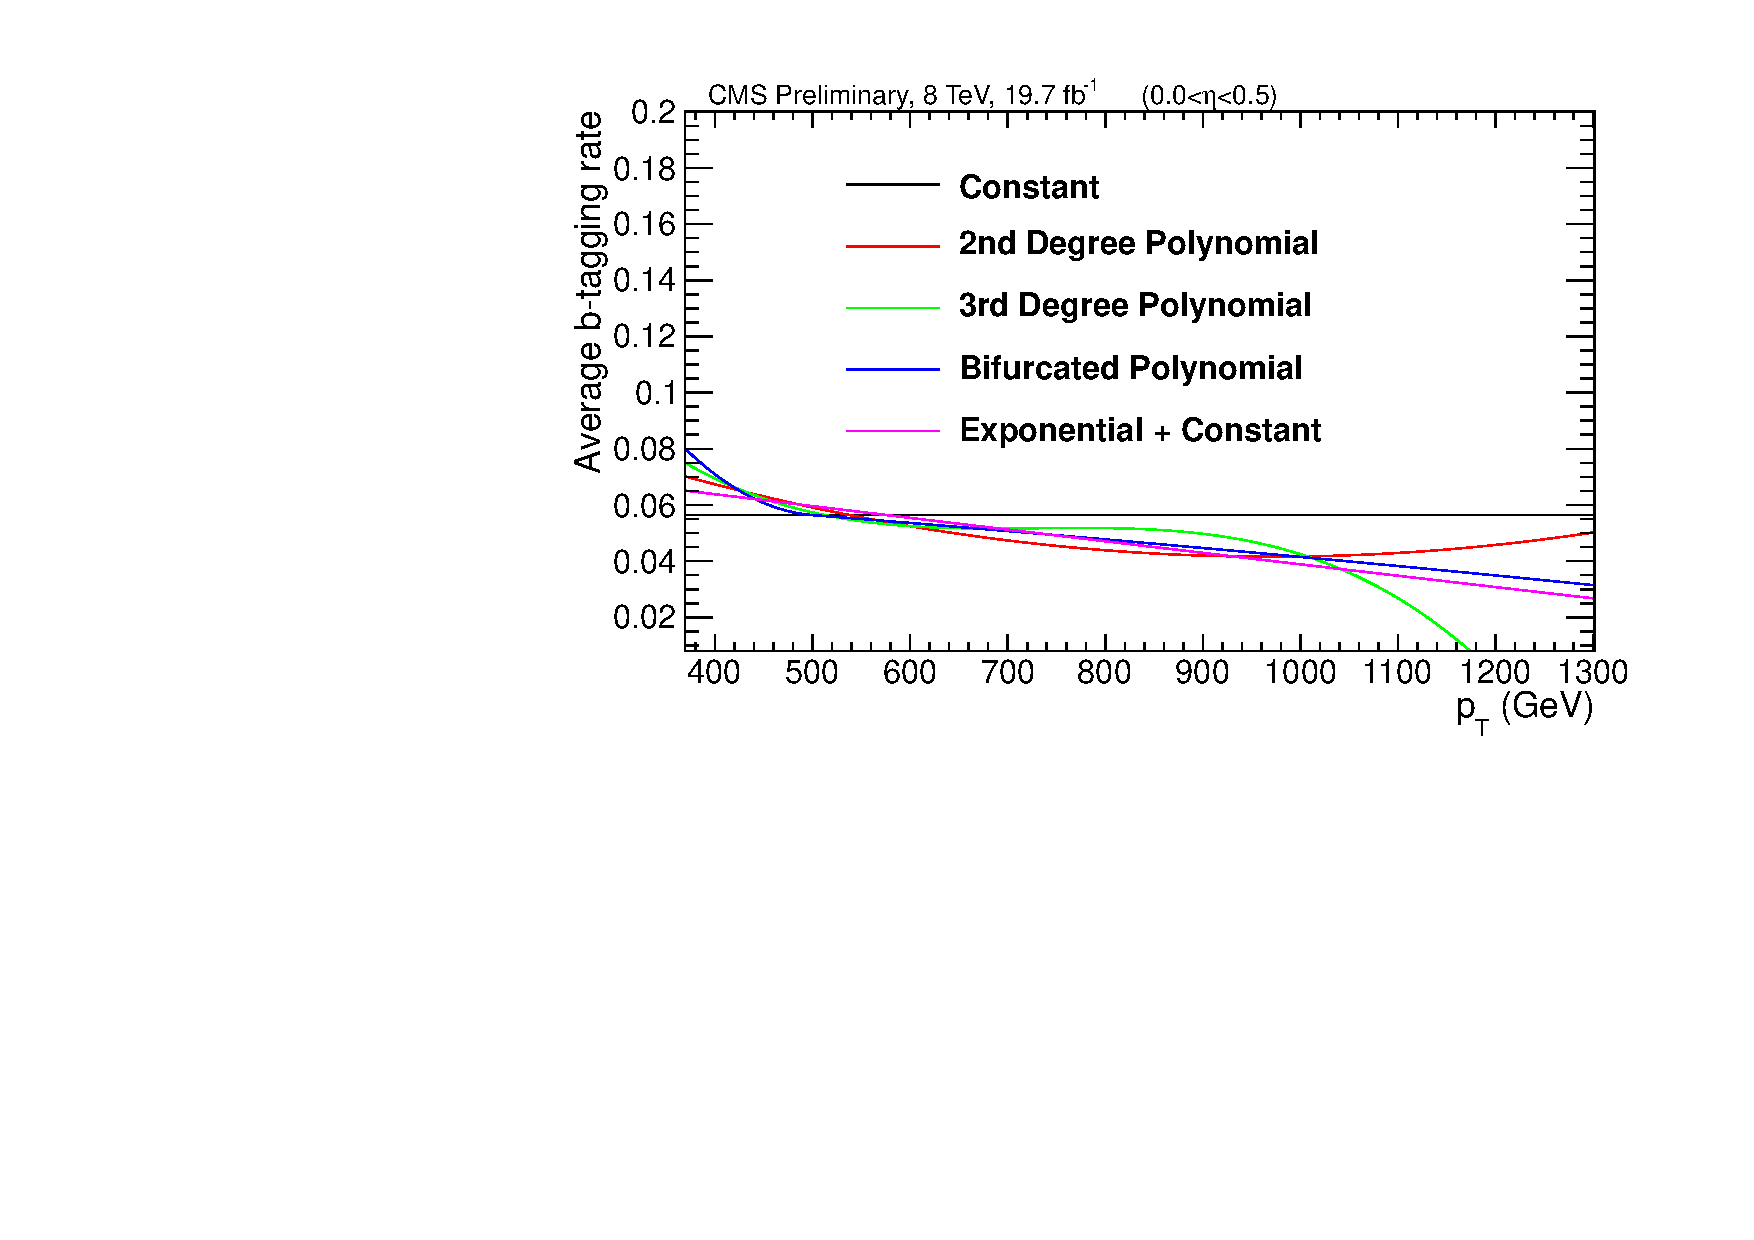
\includegraphics[width=0.7\textwidth]{AN-13-004/figs/BKGFITCOMPLOGE1.pdf}\\
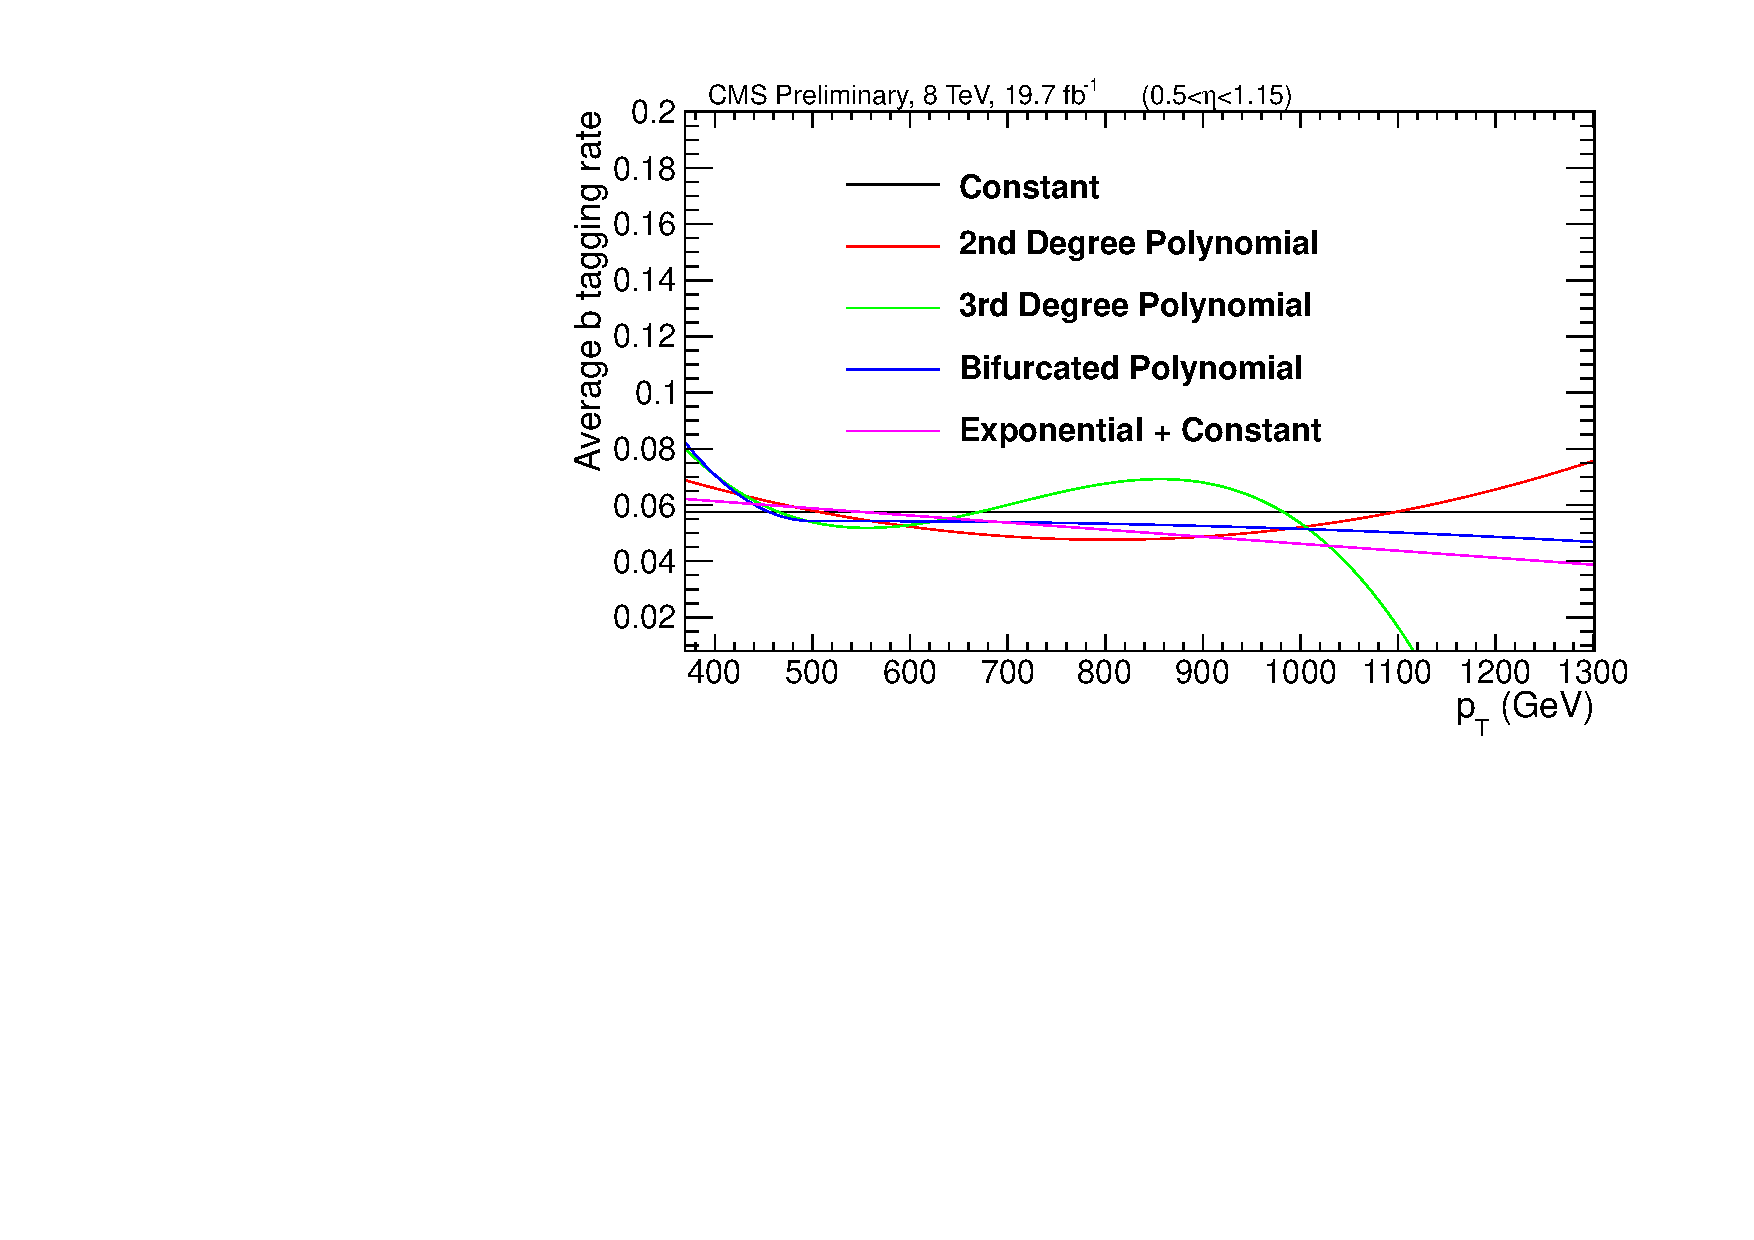
\includegraphics[width=0.7\textwidth]{AN-13-004/figs/BKGFITCOMPLOGE2.pdf}\\
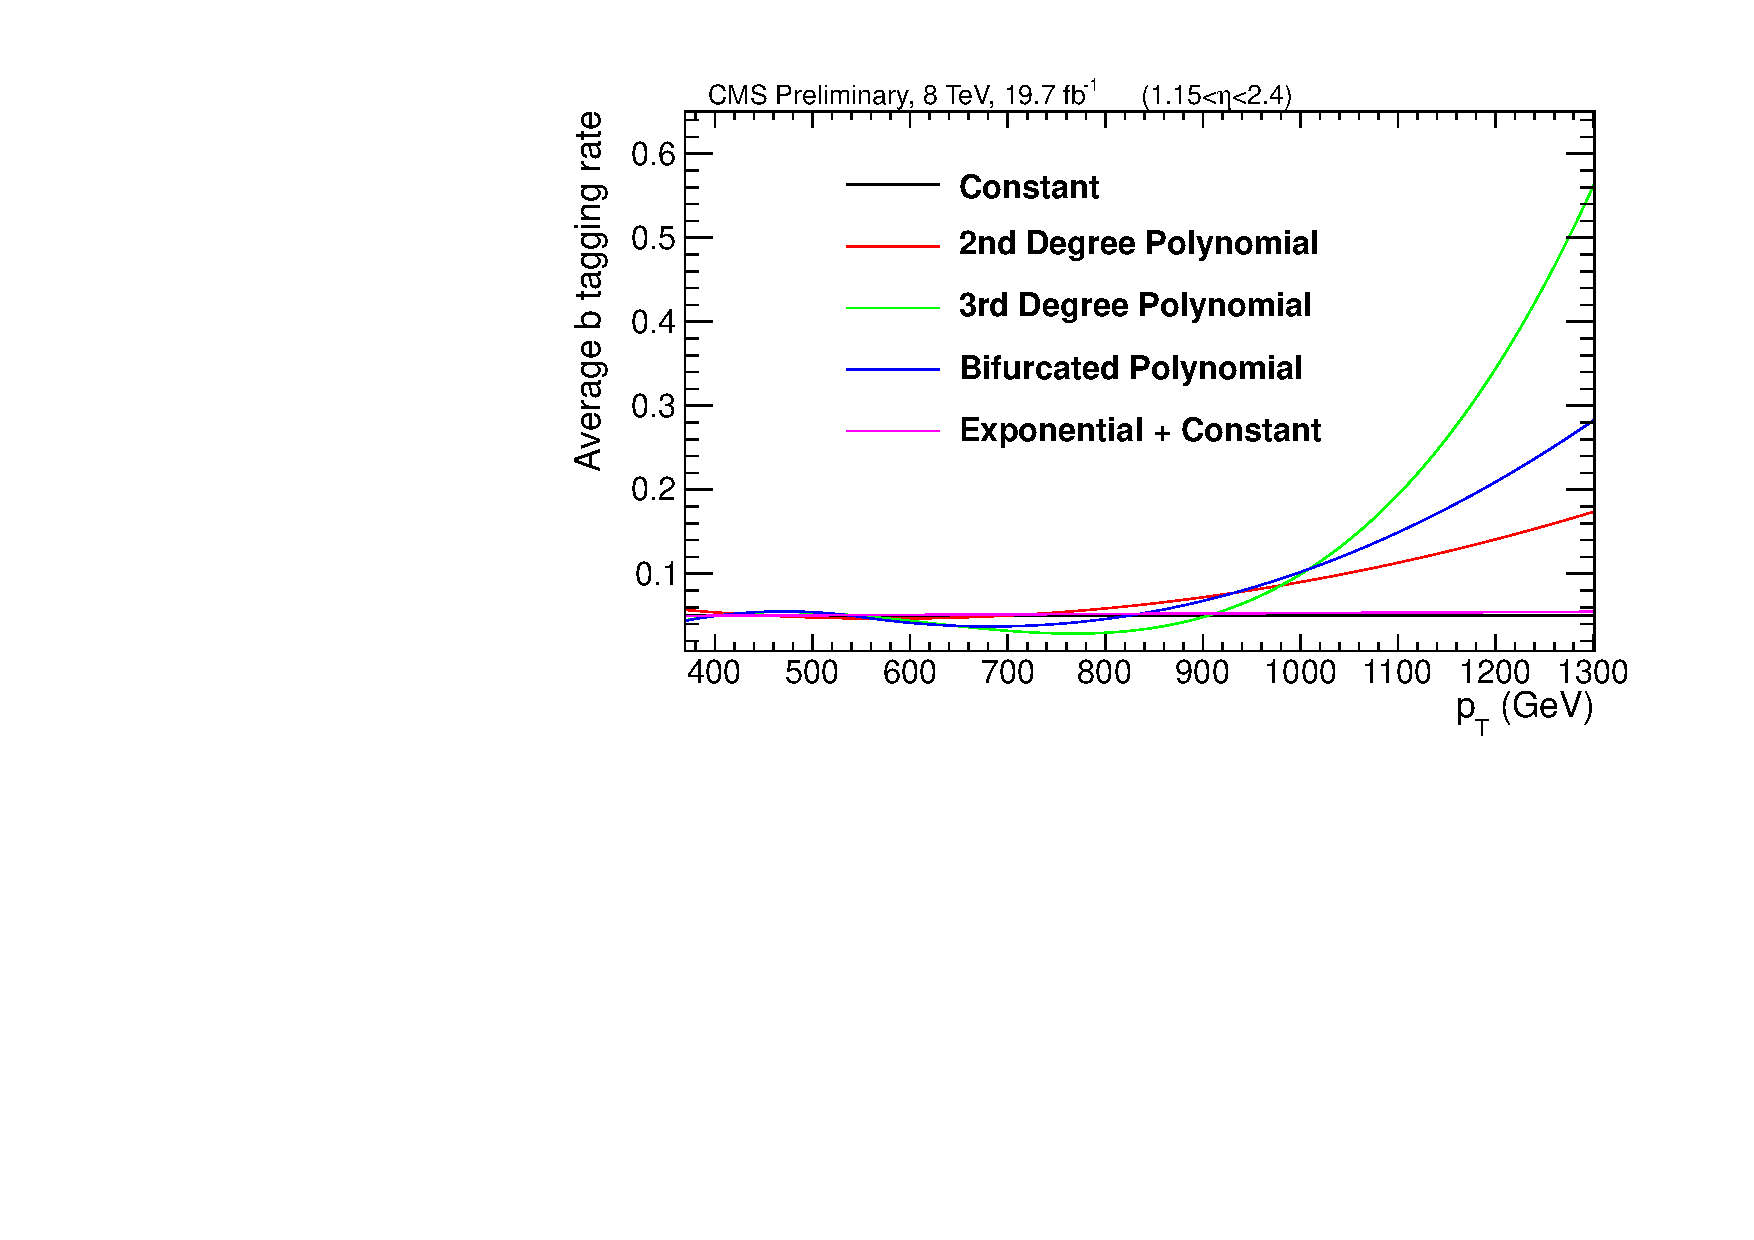
\includegraphics[width=0.7\textwidth]{AN-13-004/figs/BKGFITCOMPLOGE3.pdf}
\caption{
Alternative fit functions for the average b-tagging rate in $\eta$ regions
(a) Low
(b) Transition
(c) High
}
\label{figs:BKGFITCOMP}
\end{center}
\end{figure}

\begin{figure}[htcb]
\begin{center}
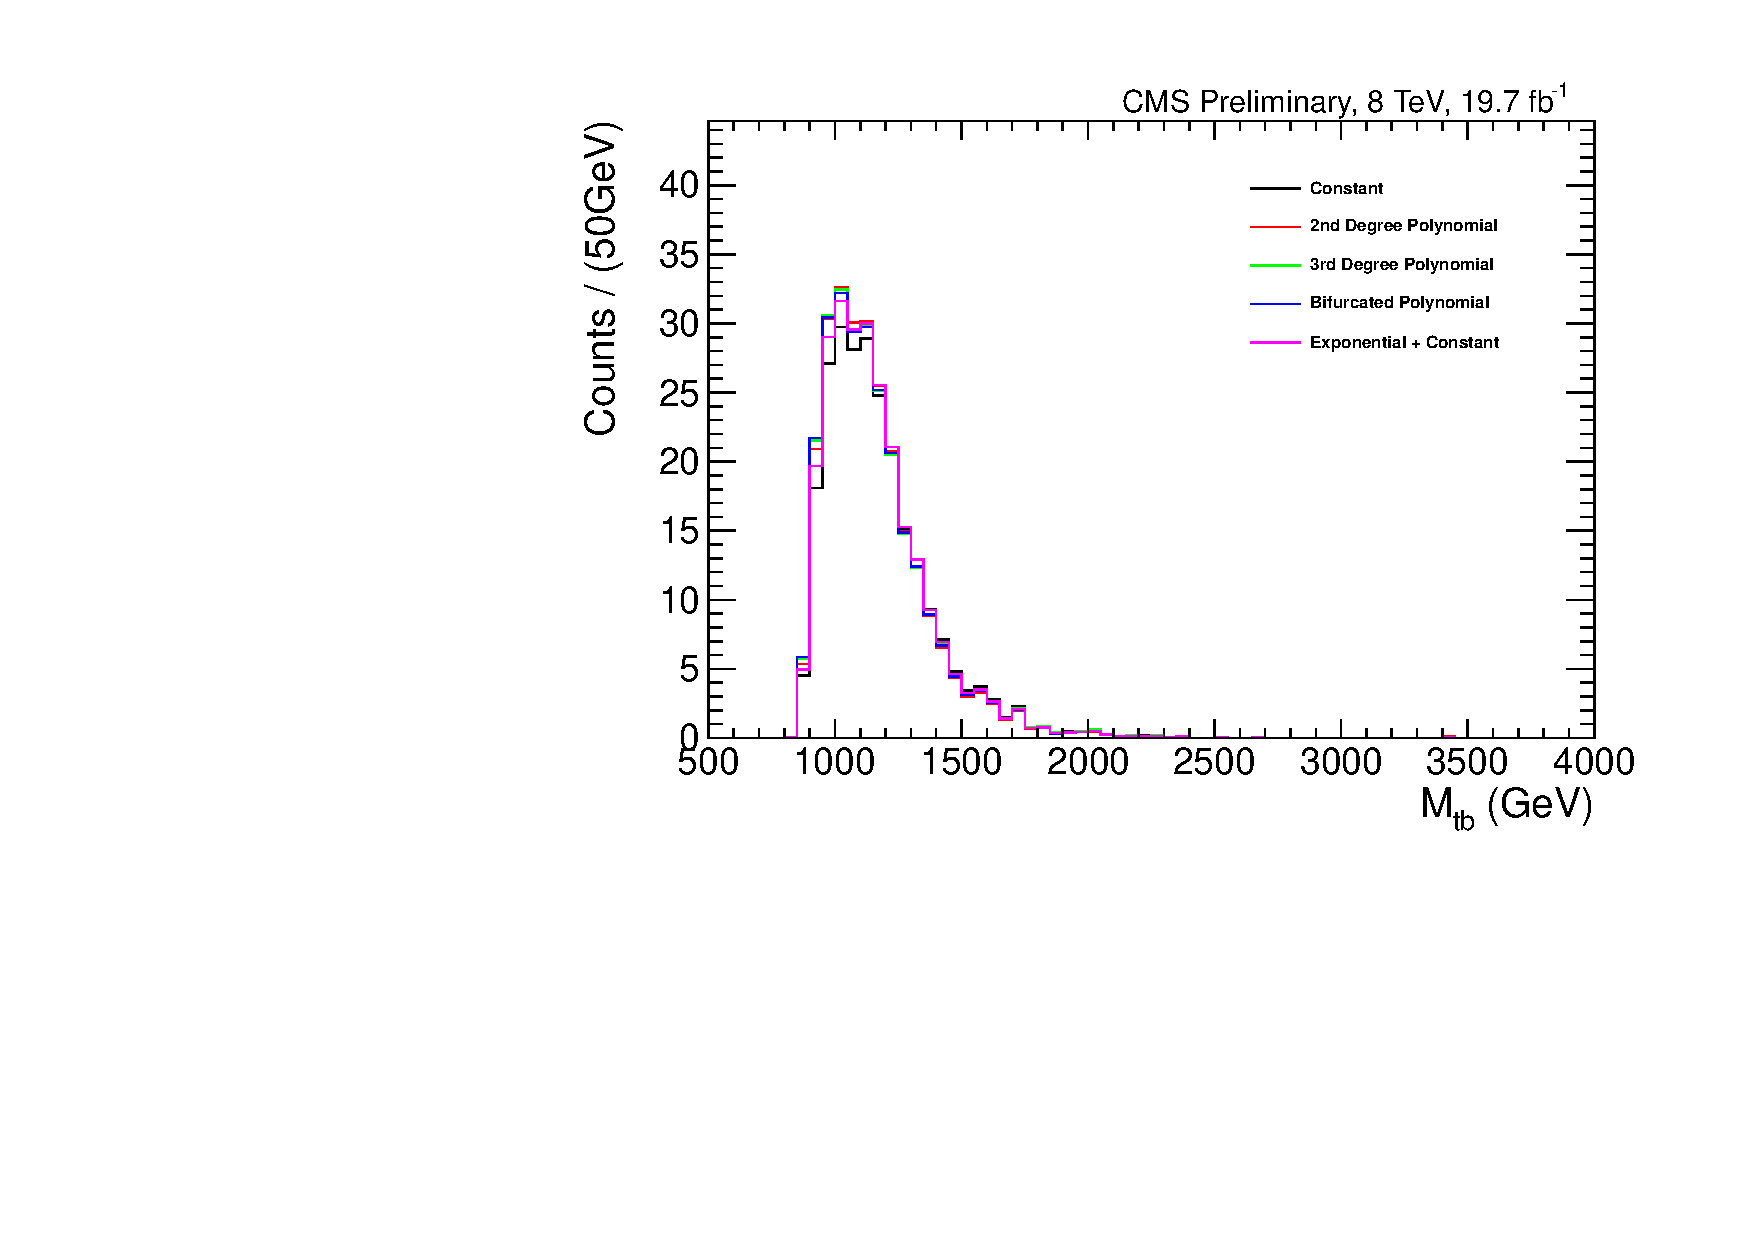
\includegraphics[width=0.7\textwidth]{AN-13-004/figs/BKGCOMP.pdf}\\
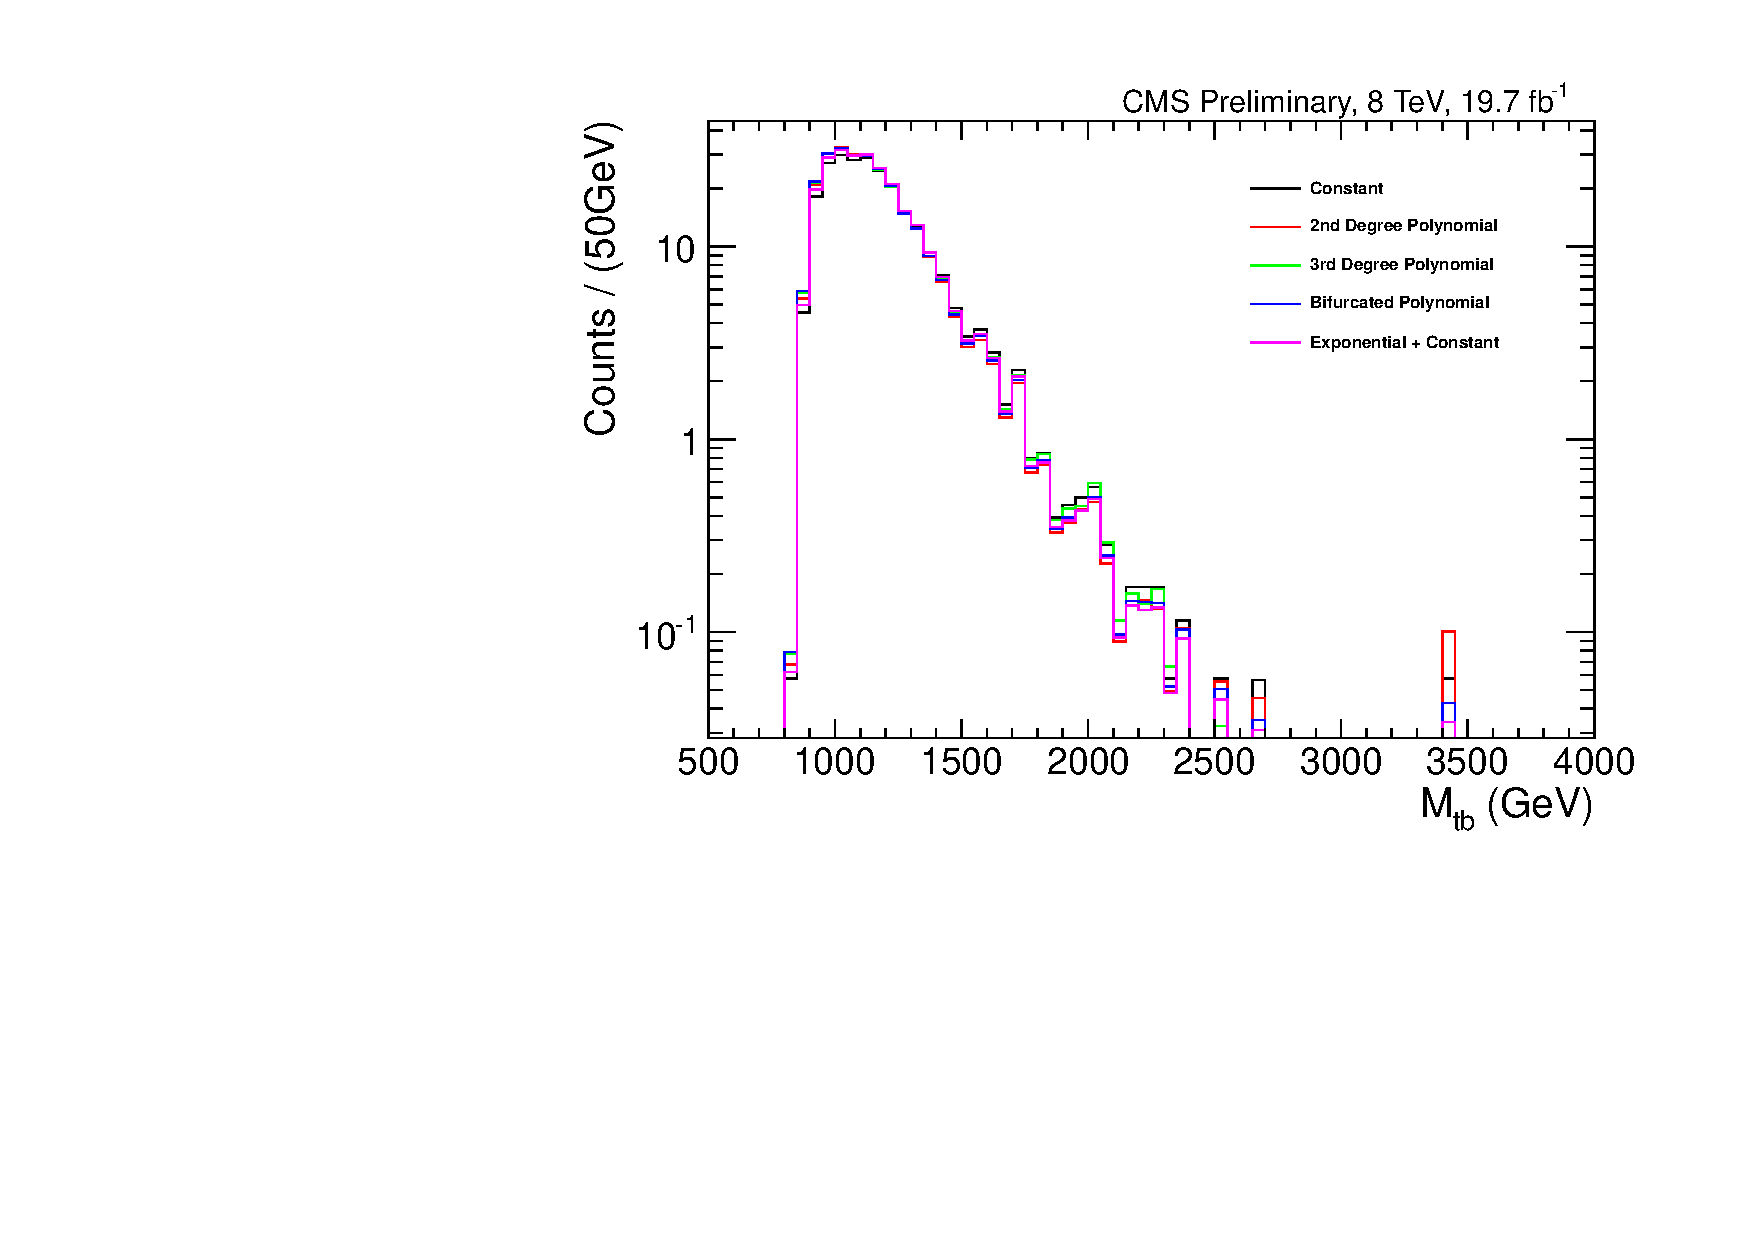
\includegraphics[width=0.7\textwidth]{AN-13-004/figs/BKGCOMPLOG.pdf}
\caption{
QCD background estimation from alternative fit functions seen in \ref{figs:BKGFITCOMP}. Top and bottom plots are the same but on linear and log y-axis scale.
}
\label{figs:BKGCOMP}
\end{center}
\end{figure}

\begin{figure}[htcb]
\begin{center}
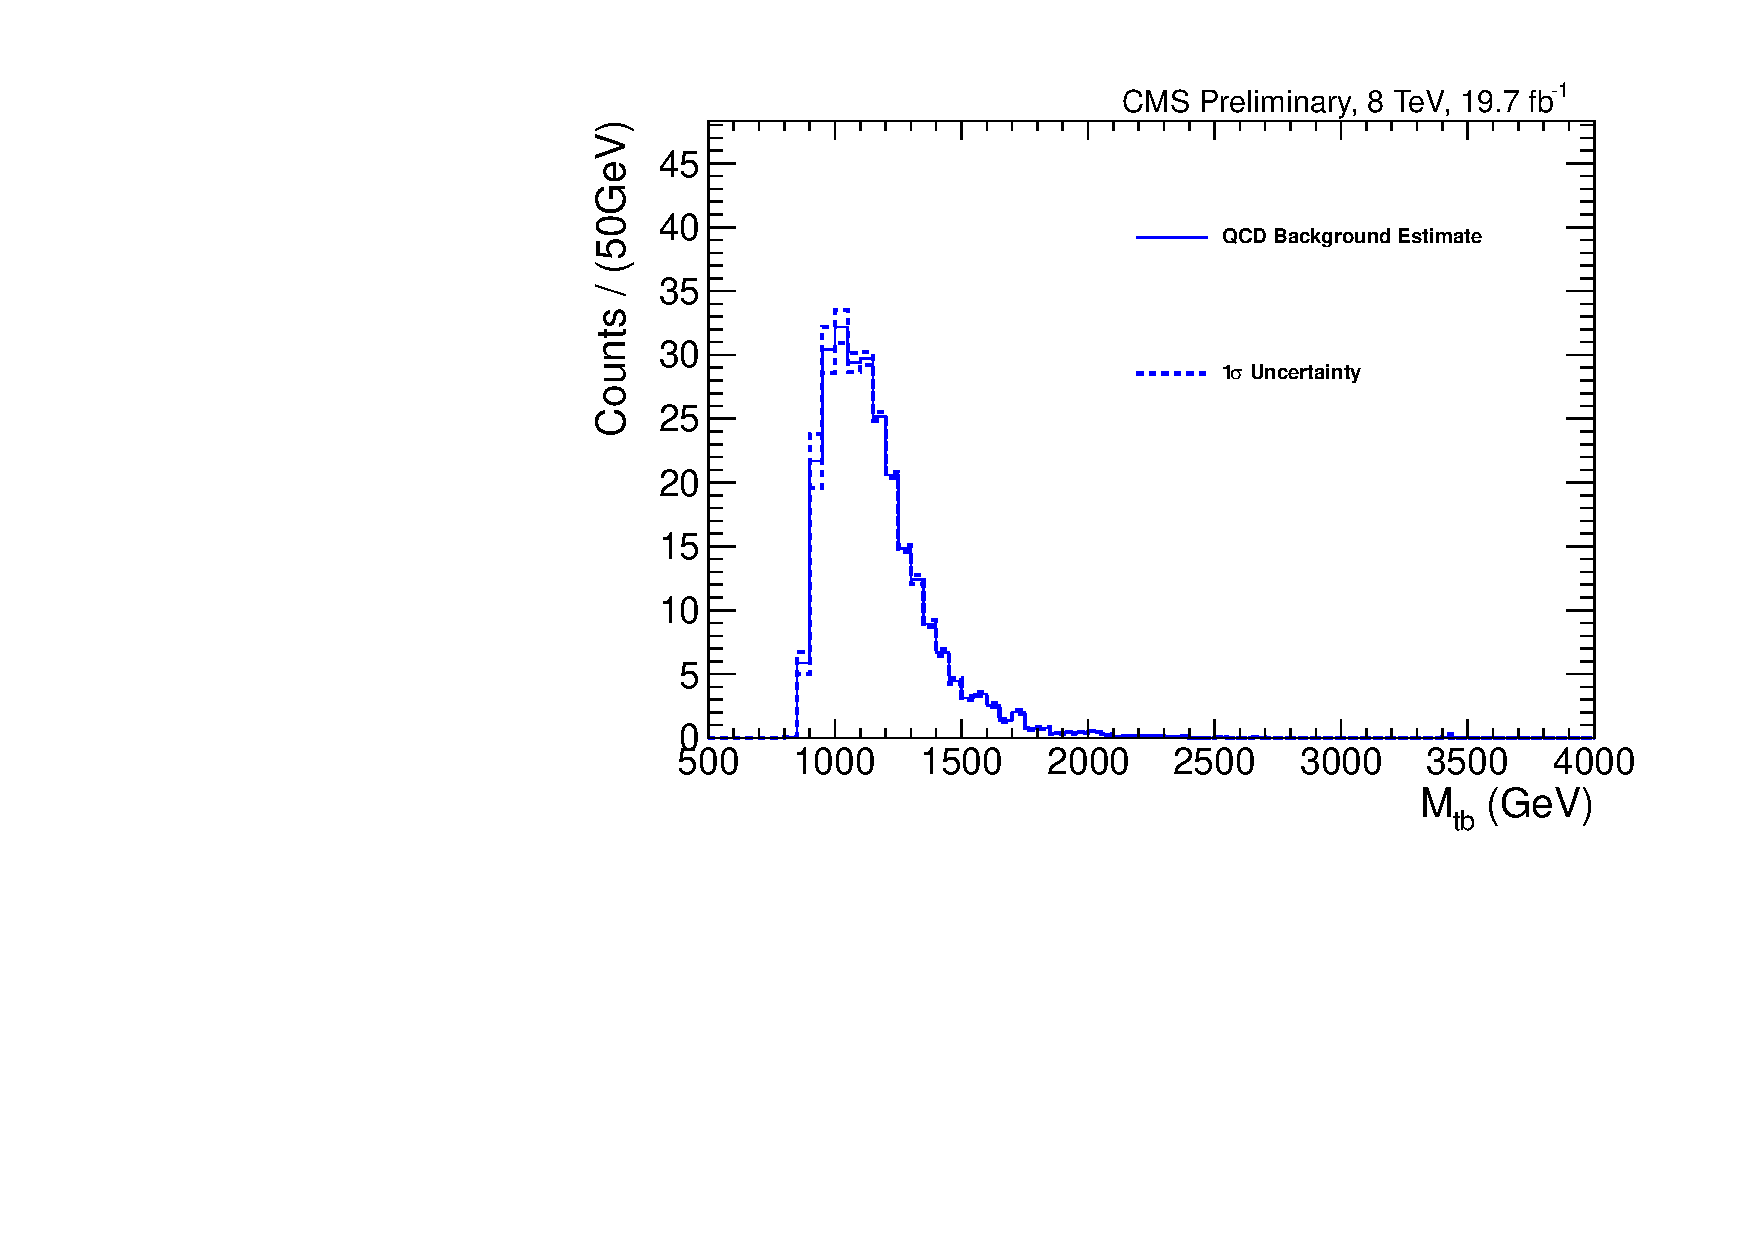
\includegraphics[width=0.7\textwidth]{AN-13-004/figs/BKGFITERR.pdf}\\
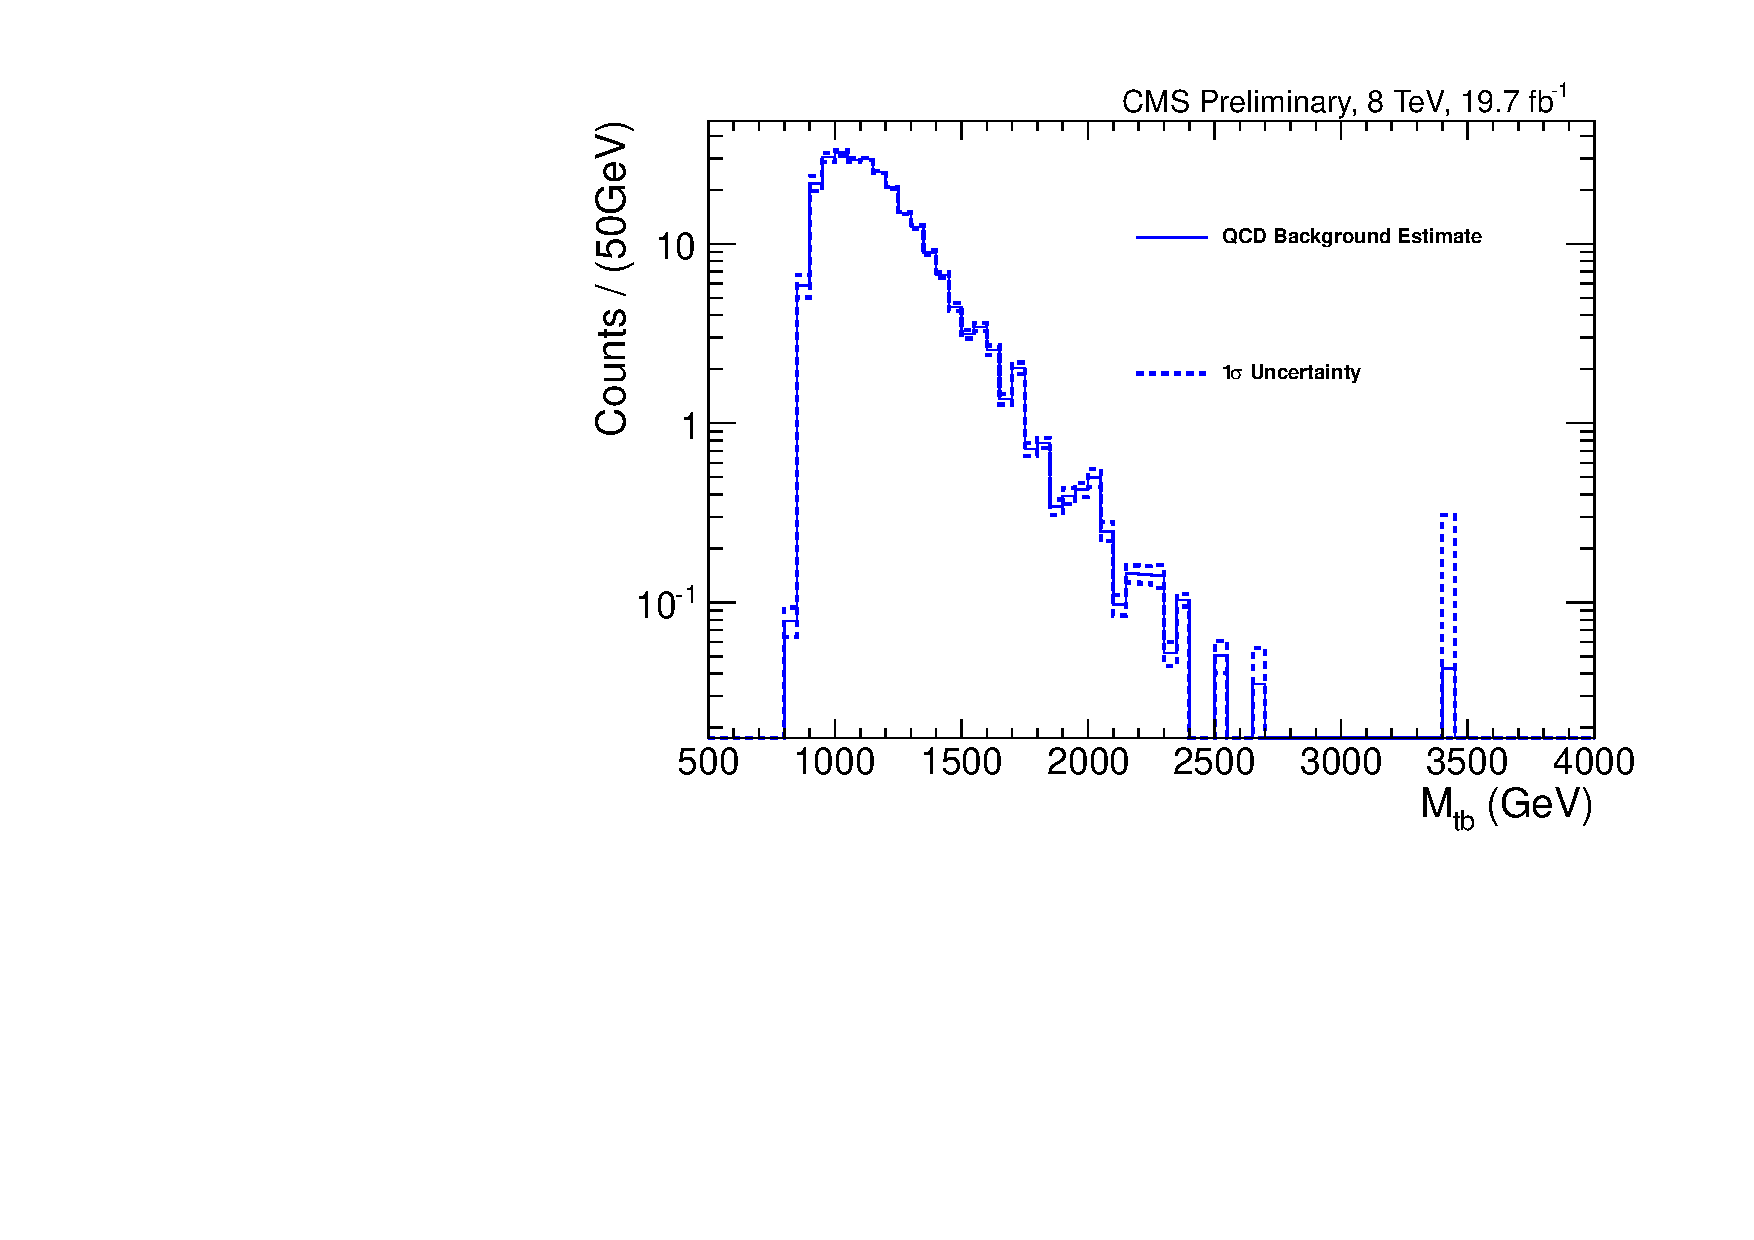
\includegraphics[width=0.7\textwidth]{AN-13-004/figs/BKGFITERRLOG.pdf}
\caption{
Uncertainty on the choice of fit as extracted from the alternative background estimations seen in \ref{figs:BKGCOMP}. Top and bottom plots are the same but on linear and log y-axis scale.
}
\label{figs:BKGERR}
\end{center}
\end{figure}

\begin{figure}[htcb]
\begin{center}
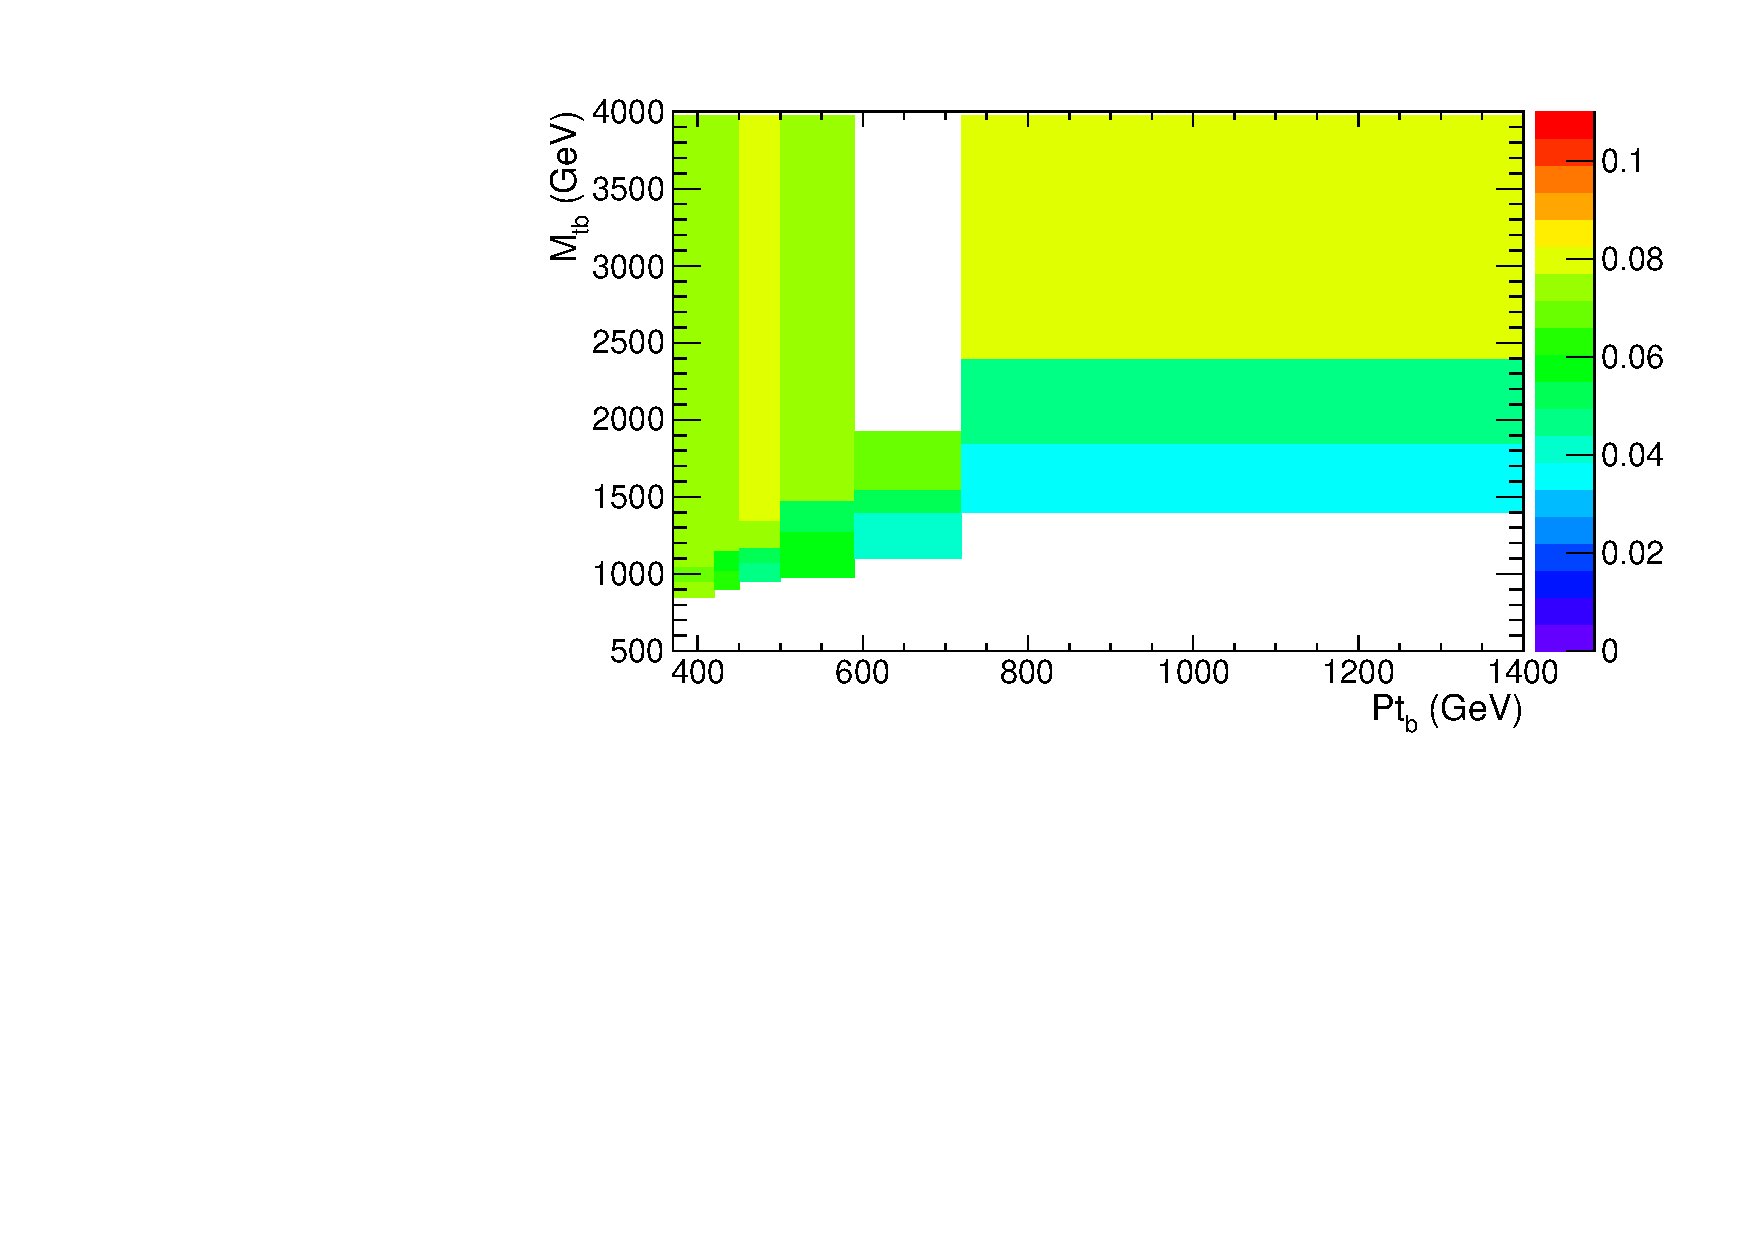
\includegraphics[width=0.7\textwidth]{AN-13-004/figs/TagrateEta1SB2dSB1.pdf}
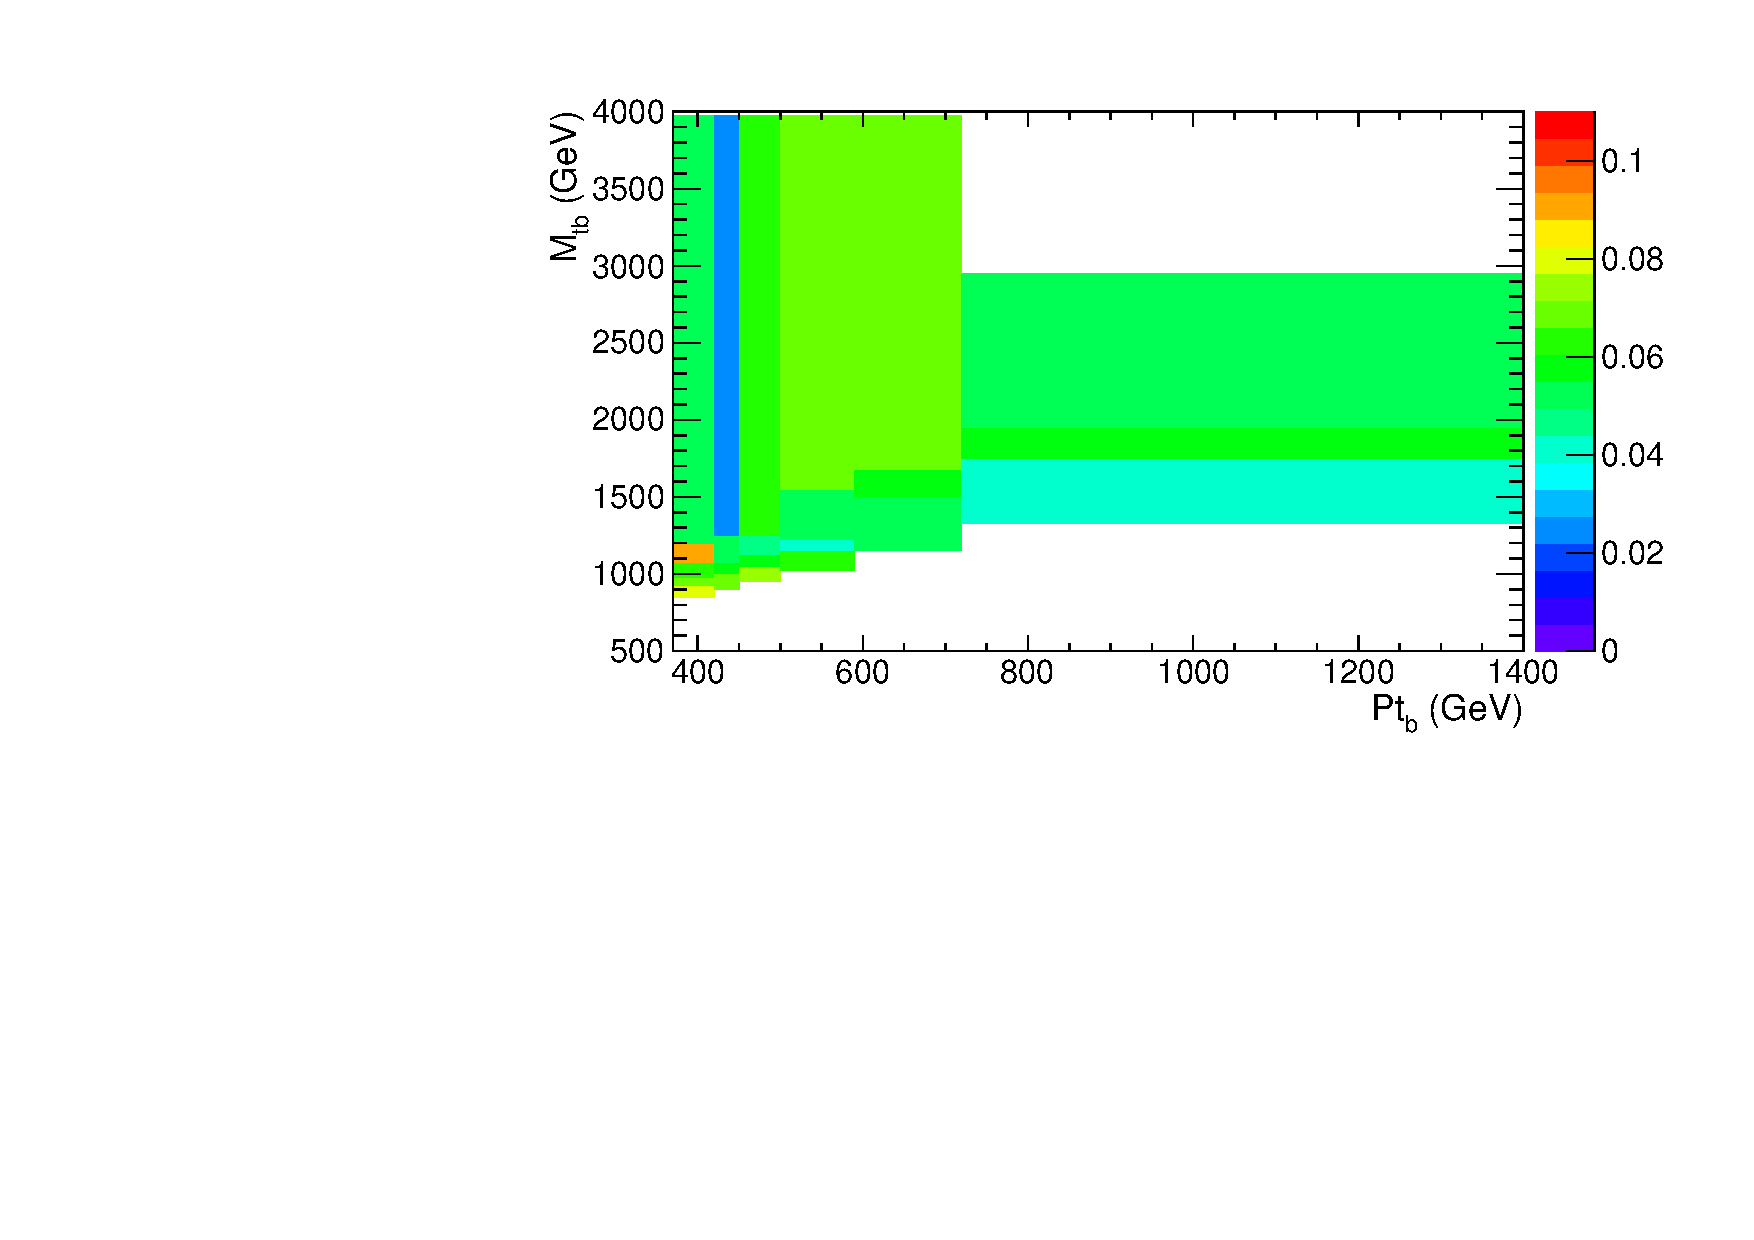
\includegraphics[width=0.7\textwidth]{AN-13-004/figs/TagrateEta2SB2dSB1.pdf}
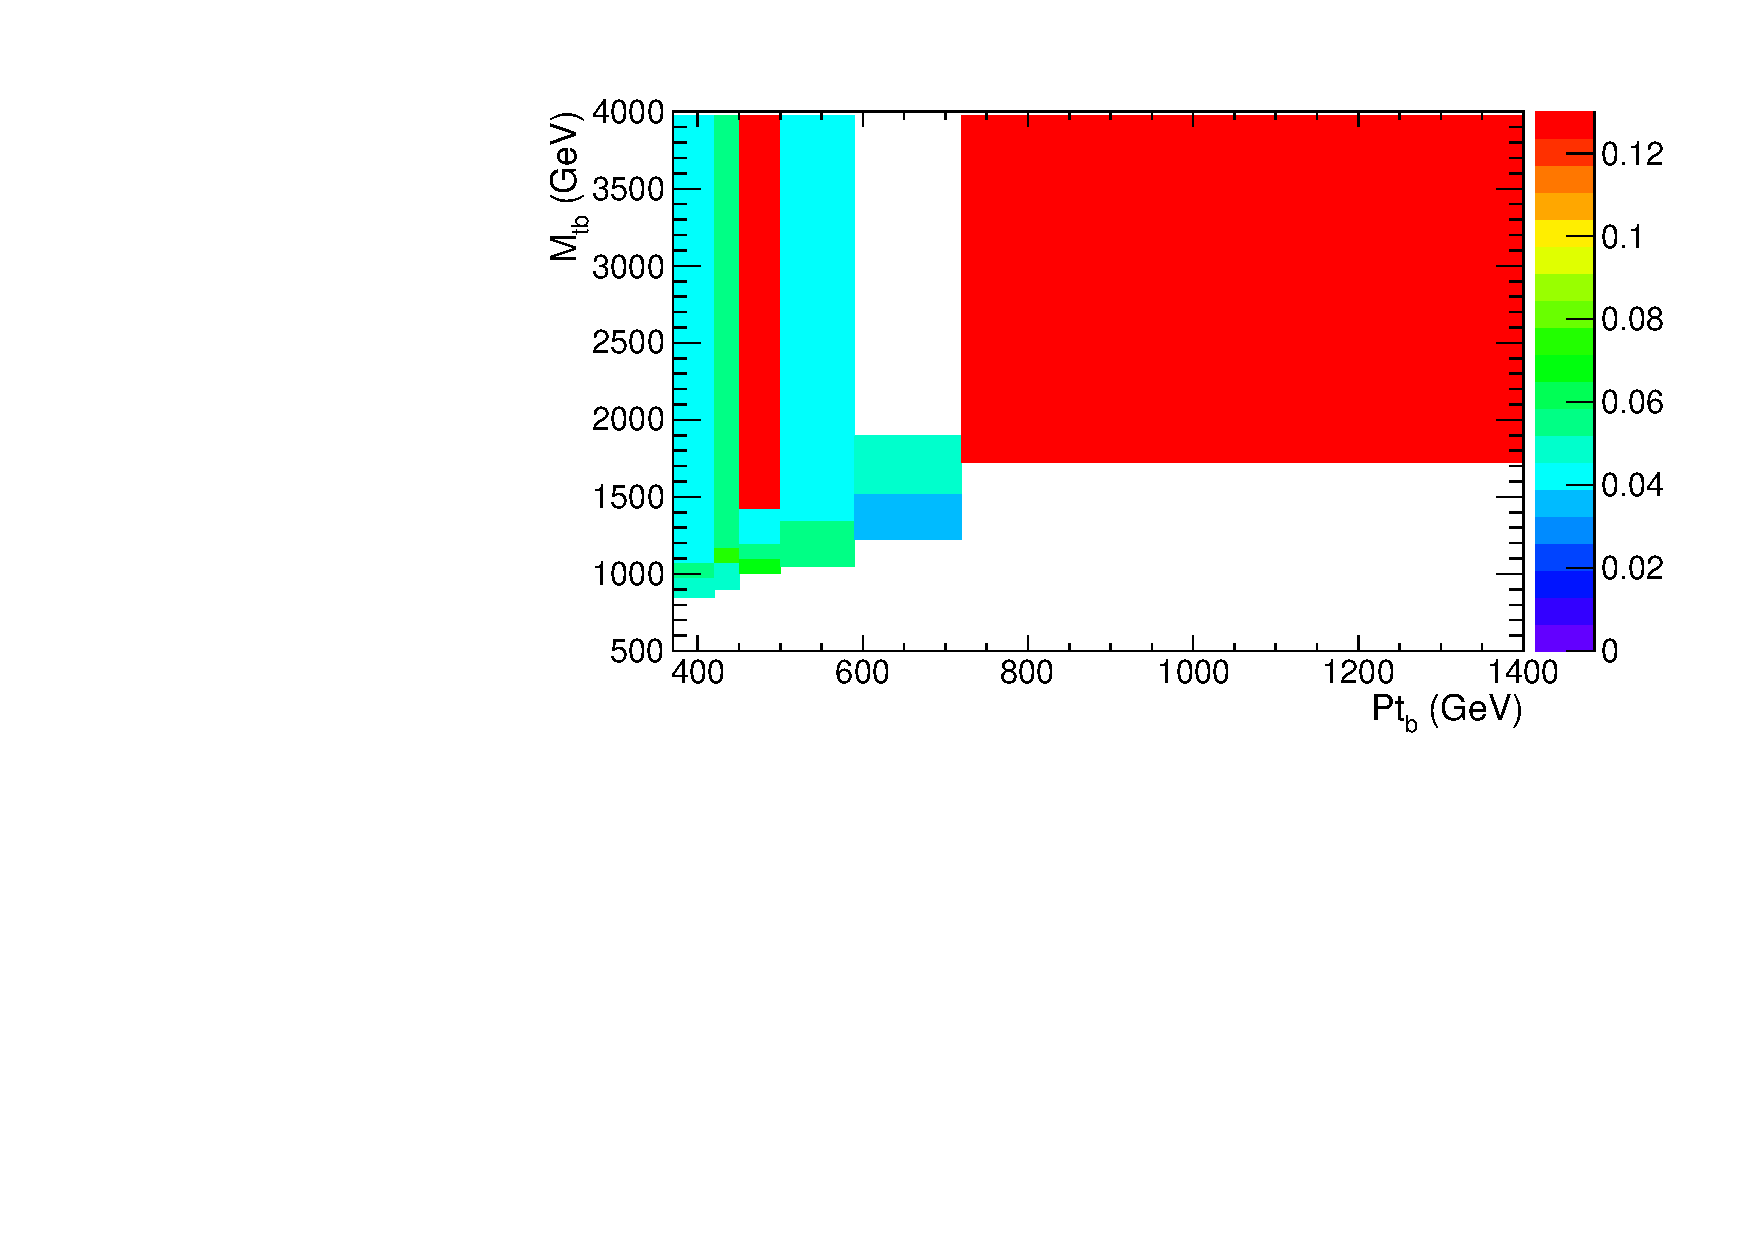
\includegraphics[width=0.7\textwidth]{AN-13-004/figs/TagrateEta3SB2dSB1.pdf}
\caption{
Two dimensional parameterization of average b-tagging rate in $p_{T_{b}}$ and $\mathrm{M_{tb}}$.  The x axis binning is identical to the binning in Chapter \ref{sec:backgroundEstimation}.  
The y-axis is binned adaptively to approximate equivalent statistics over each y-axis bin per x axis bin. 
(a) Low $\eta$ Region
(b) Transition $\eta$ Region
(c) High $\eta$ Region
}
\label{figs:sb2deta}
\end{center}
\end{figure}

\begin{figure}[htcb]
\begin{center}
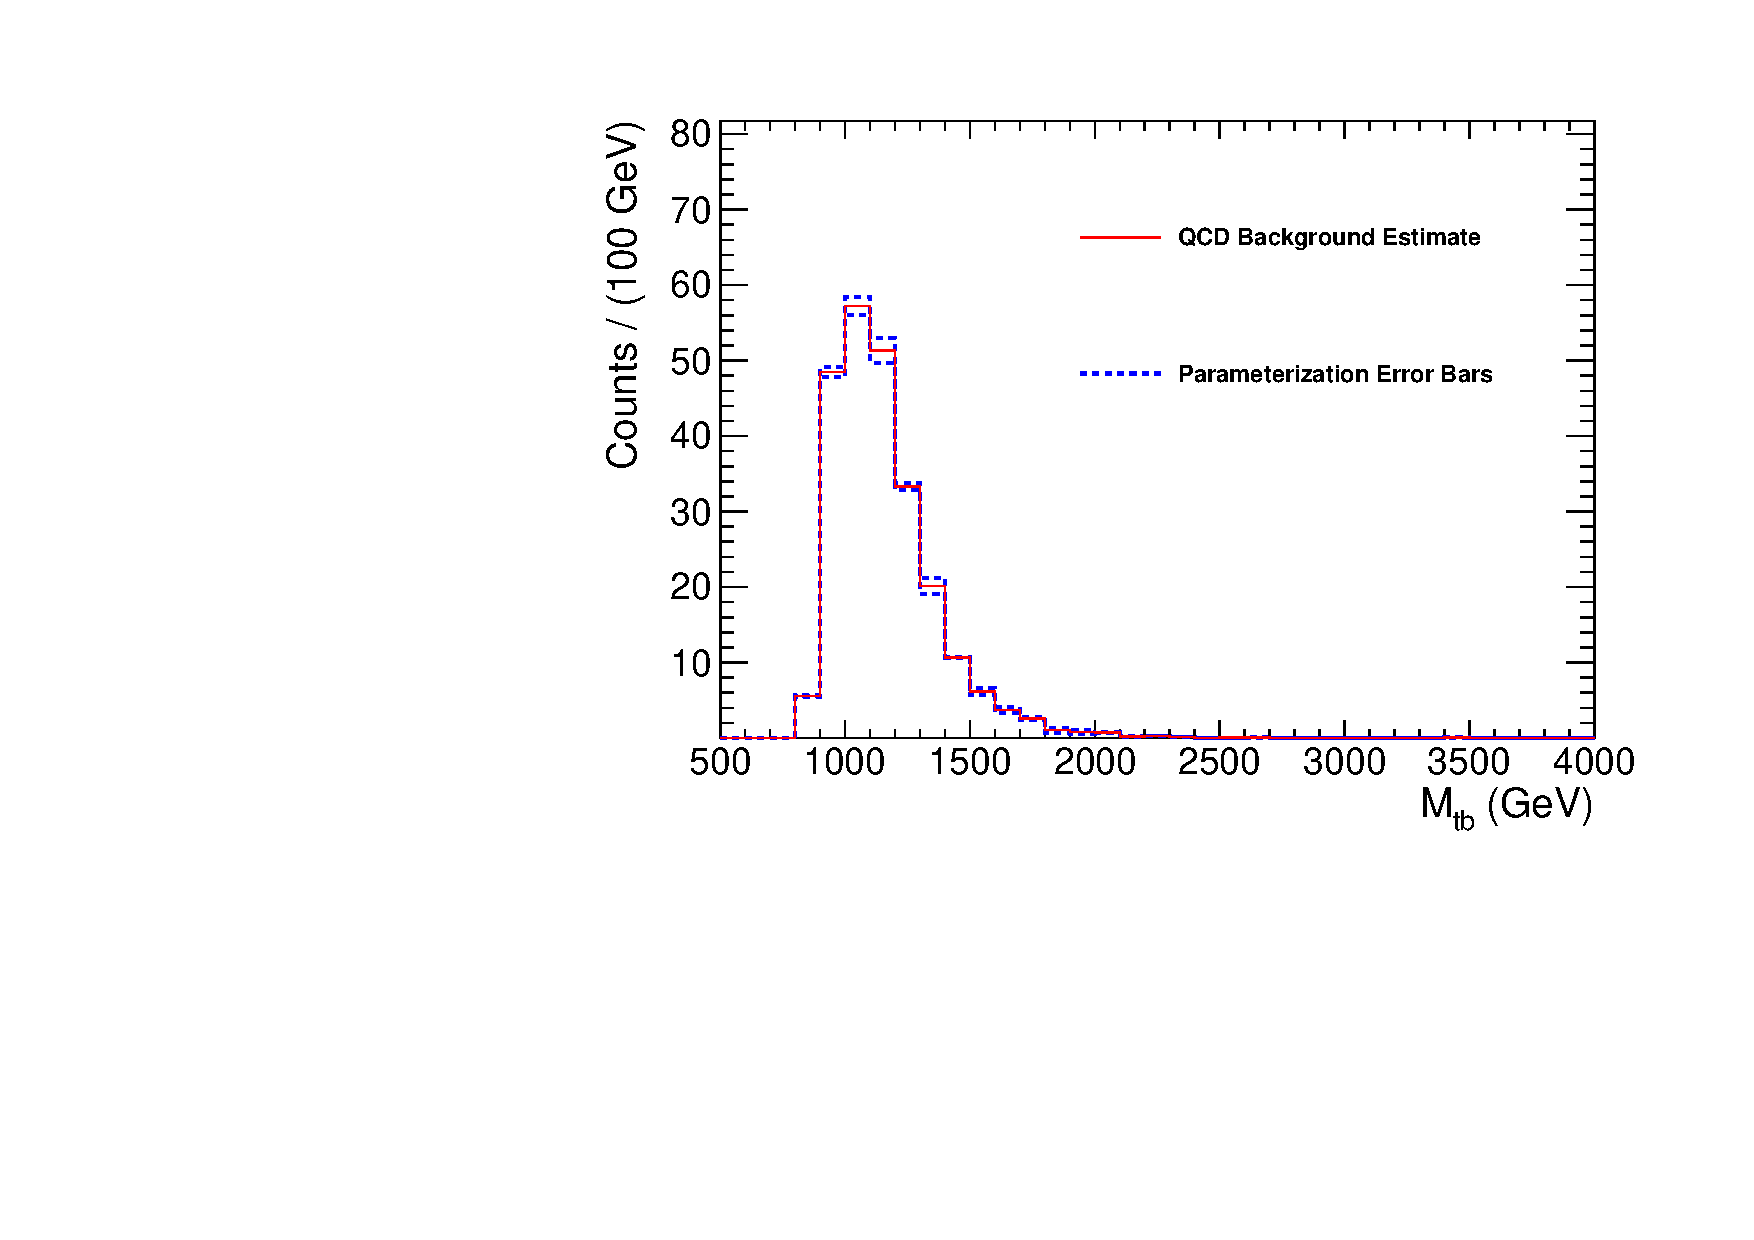
\includegraphics[width=0.7\textwidth]{AN-13-004/figs/Mtb2dvs1dBE}\\
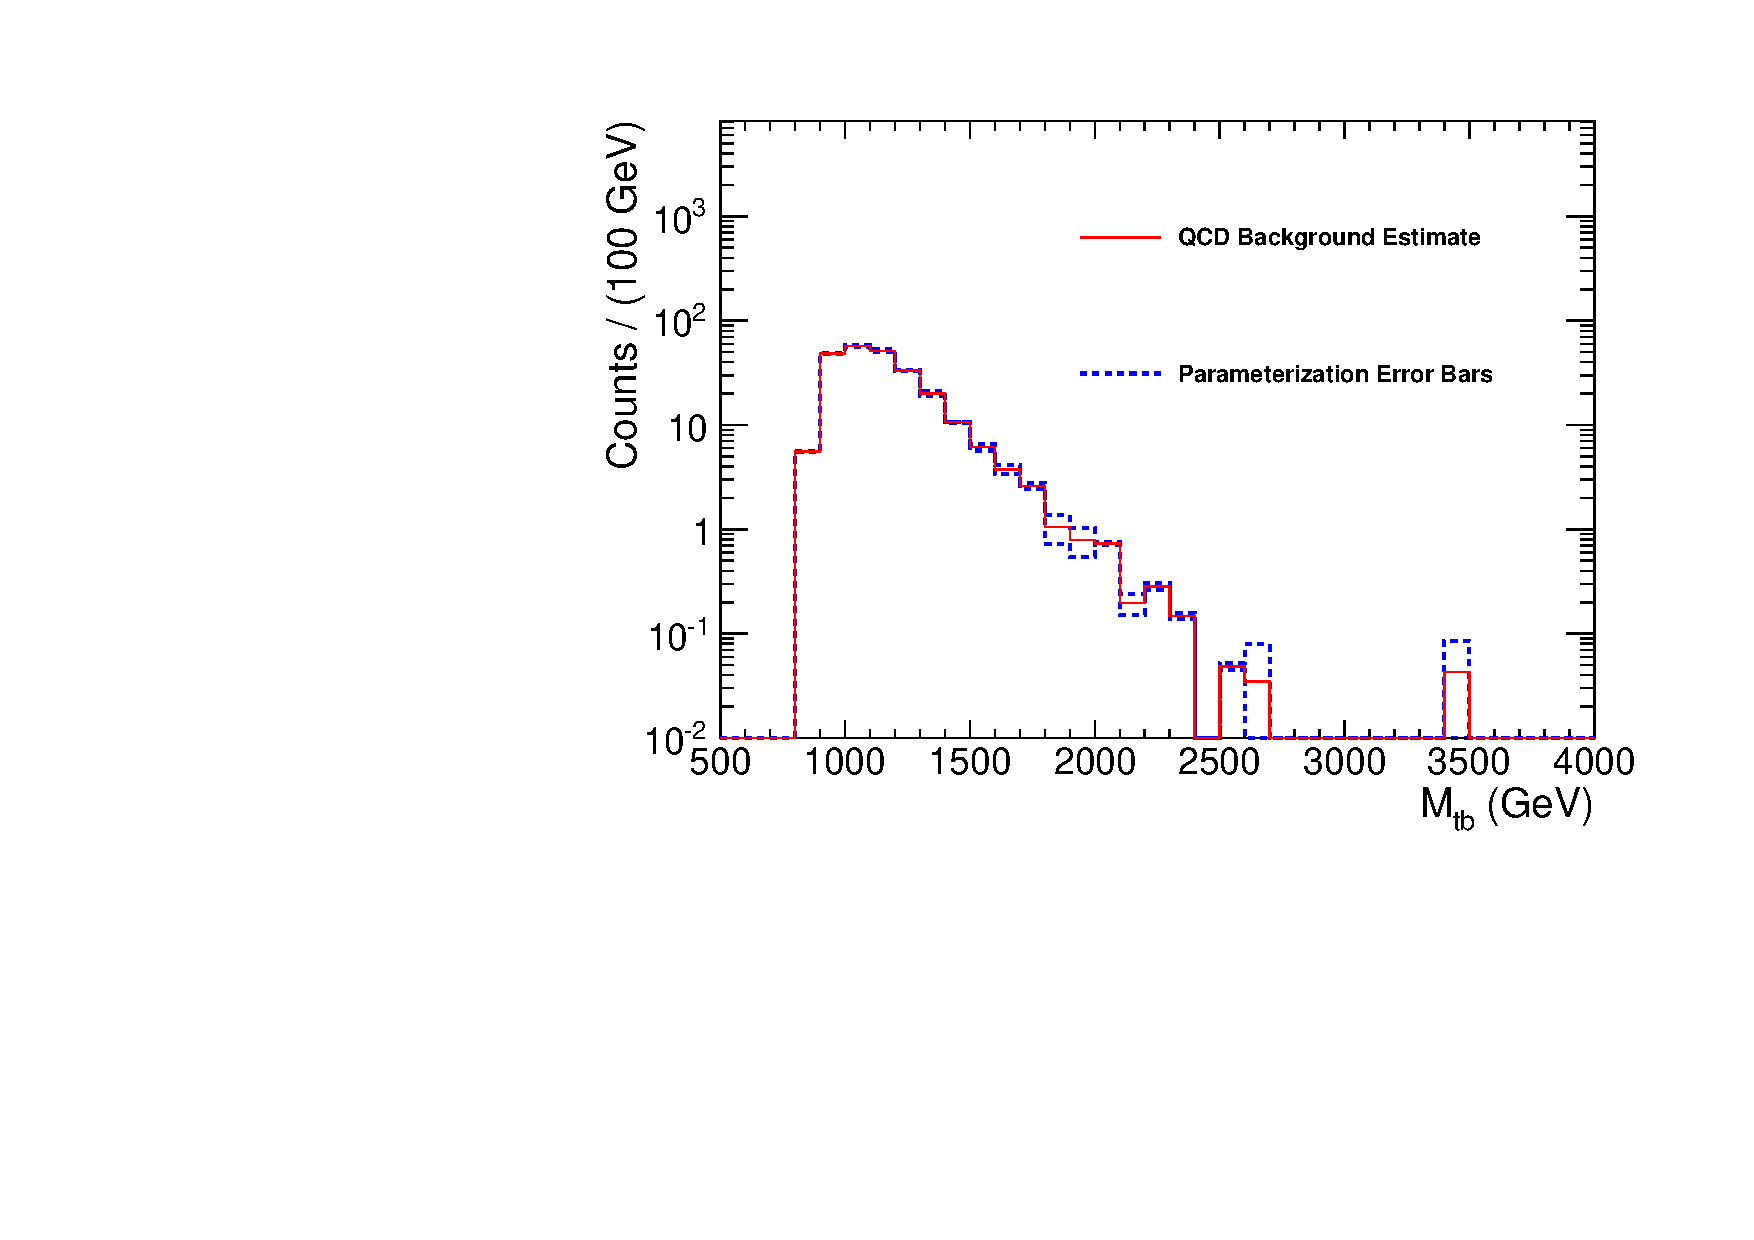
\includegraphics[width=0.7\textwidth]{AN-13-004/figs/Mtb2dvs1dBEsemilog}
\caption{
Uncertainty on the parameterization choice. Top and bottom plots are the same but on linear and log y-axis scale.
}
\label{figs:PARAMERROR}
\end{center}
\end{figure}


